
% ----------------------------------------------------------------------
%                   LATEX TEMPLATE FOR PhD THESIS
% ----------------------------------------------------------------------

% based on Harish Bhanderi's PhD/MPhil template, then Uni Cambridge
% http://www-h.eng.cam.ac.uk/help/tpl/textprocessing/ThesisStyle/
% corrected and extended in 2012 by Stylianos Kyriacou



%: Style file for Latex
% Most style definitions are in the external file PhDthesisPSnPDF.
% In this template package, it can be found in ./Latex/Classes/
%\documentclass[twoside,11pt]{Latex/Classes/PhDthesisPSnPDF}
\documentclass[twoside,12pt]{Latex/Classes/PhDthesisPSnPDF}
\usepackage{setspace}
\usepackage{placeins} 

%For watermark uncomment the last 3 lines
%\usepackage{draftwatermark}
%\SetWatermarkText{DRAFT}
%\SetWatermarkScale{5}

%for corrections 
%\doublespacing

%: Colore or not 
% Change comments accourtigly for B/W or Colored copies 
\newif\ifcolore
%\coloretrue
\colorefalse

%: Macro file for Latex
% Macros help you summarise frequently repeated Latex commands.
% Here, they are placed in an external file /Latex/Macros/MacroFile1.tex
% An macro that you may use frequently is the figuremacro (see introduction.tex)
% This file contains macros that can be called up from connected TeX files
% It helps to summarise repeated code, e.g. figure insertion (see below).

% insert a centered figure with caption and description
% parameters 1:filename, 2:title, 3:description and label
\newcommand{\figuremacro}[3]{
	\begin{figure}[htbp]
		\centering
		\includegraphics[width=1\textwidth]{#1}
		\caption[#2]{\textbf{#2} - #3}
		\label{#1}
	\end{figure}
}

% insert a centered figure with caption and description AND WIDTH
% parameters 1:filename, 2:title, 3:description and label, 4: textwidth
% textwidth 1 means as text, 0.5 means half the width of the text
\newcommand{\figuremacroW}[4]{
	\begin{figure}[htbp]
		\centering
		\includegraphics[width=#4\textwidth]{#1}
		\caption[#2]{\textbf{#2} - #3}
		\label{#1}
	\end{figure}
}

% inserts a figure with wrapped around text; only suitable for NARROW figs
% o is for outside on a double paged document; others: l, r, i(inside)
% text and figure will each be half of the document width
% note: long captions often crash with adjacent content; take care
% in general: above 2 macro produce more reliable layout
\newcommand{\figuremacroN}[3]{
	\begin{wrapfigure}{o}{0.5\textwidth}
		\centering
		\includegraphics[width=0.48\textwidth]{#1}
		\caption[#2]{{\small\textbf{#2} - #3}}
		\label{#1}
	\end{wrapfigure}
}

% predefined commands by Harish
\newcommand{\PdfPsText}[2]{
  \ifpdf
     #1
  \else
     #2
  \fi
}

\newcommand{\IncludeGraphicsH}[3]{
  \PdfPsText{\includegraphics[height=#2]{#1}}{\includegraphics[bb = #3, height=#2]{#1}}
}

\newcommand{\IncludeGraphicsW}[3]{
  \PdfPsText{\includegraphics[width=#2]{#1}}{\includegraphics[bb = #3, width=#2]{#1}}
}

\newcommand{\InsertFig}[3]{
  \begin{figure}[!htbp]
    \begin{center}
      \leavevmode
      #1
      \caption{#2}
      \label{#3}
    \end{center}
  \end{figure}
}


%%% Local Variables: 
%%% mode: latex
%%% TeX-master: "~/Documents/LaTeX/CUEDThesisPSnPDF/thesis"
%%% End: 

\usepackage{amsmath}
\usepackage{amssymb}
\usepackage{mathrsfs}
%: ----------------------------------------------------------------------
%:                  TITLE PAGE: name, degree,..
% ----------------------------------------------------------------------
% below is to generate the title page with crest and author name

%if output to PDF then put the following in PDF header
\ifpdf  
    \pdfinfo { /Title  (Evolutionary Algorithm-based Design-Optimization Methods in Turbomachinery)
               /Creator (Stylianos Kyriacou )
               /Producer (Stylianos Kyriacou )
               /Author (Stylianos Kyriacou stelios.kyriacou@gmail.com)
               /CreationDate (D:YYYYMMDDhhmmss)  %format D:YYYYMMDDhhmmss
               /ModDate (D:YYYYMMDDhhmm)
               /Subject (Evolutionary Algorithm-based Design-Optimization Methods in Turbomachinery)
               /Keywords (Optimization, Evolutionary Algorithms, Metamodels, Turbo-machinery) }
    \pdfcatalog { /PageMode (/UseOutlines)
                  /OpenAction (fitbh)  }
\fi


\title{Evolutionary Algorithm-based Design-Optimization Methods in Turbomachinery}



% ----------------------------------------------------------------------
% The section below defines www links/email for author and institutions
% They will appear on the title page of the PDF and can be clicked
\ifpdf
  \author{\href{mailto:stelios.kyriacou@gmail.com}{Stylianos Kyriacou}}
%  \cityofbirth{born in XYZ} % uncomment this if your university requires this
%  % If city of birth is required, also uncomment 2 sections in PhDthesisPSnPDF
%  % Just search for the "city" and you'll find them.
  \collegeordept{\href{http://www.ntua.gr}{Mechanical Engineering}}
  \university{\href{http://www.ntua.gr}{National Technical University of Athens}}

  % The crest is a graphics file of the logo of your research institution.
  % Place it in ./0_frontmatter/figures and specify the width
  \crest{\includegraphics[width=4cm]{pyrforos}}
  
% If you are not creating a PDF then use the following. The default is PDF.
\else
  \author{Stylianos Kyriacou}
%  \cityofbirth{born in XYZ}
  \collegeordept{Mechanical Engineering, Parallel CFD \& Optimization Unit.}
  \university{National Technical University of Athens.}
  \crest{\includegraphics[width=4cm]{pyrforos}}
\fi

%\renewcommand{\submittedtext}{change the default text here if needed}
\degree{Philosophi\ae Doctor (PhD)}
\degreedate{year month}


% ----------------------------------------------------------------------
       
% turn of those nasty overfull and underfull hboxes
\hbadness=10000
\hfuzz=50pt


%: --------------------------------------------------------------
%:                  FRONT MATTER: dedications, abstract,..
% --------------------------------------------------------------

\begin{document}

%\language{english}

% sets line spacing
\renewcommand\baselinestretch{1.0}
\baselineskip=18pt plus1pt
%\onehalfspace 
\singlespace 

%: ----------------------- generate cover page ------------------------

%\maketitle  % command to print the title page with above variables

%
\begin{titlepage}
\thispagestyle{empty}
%
%
%
\begin{flushleft}
\mbox{
\begin{minipage}[c]{0.20\textwidth}
%   \scalebox{.15}{\epsfig{file=pyrforos.eps}}
   \scalebox{.20}{\includegraphics{pyrforos}}
\end{minipage}
\begin{minipage}[c]{30em}
   \raggedright
   \sc \bf
   {\large National Technical University of Athens} \\
   School of Mechanical Engineering \\
   Department of Fluids \\
   Lab of Thermal Turbomachines\\
   Parallel CFD \& Optimization Unit\\
\end{minipage}
}
\end{flushleft}

\vskip  3cm

\begin{center}
{\large \bf Evolutionary Algorithm-based Design-Optimization Methods in Turbomachinery}
\vskip  2cm
A Thesis Submitted to the National Technical University of Athens
for the degree of Doctor of Philosophy
in the Faculty of Mechanical Engineering
\vskip  1cm
{\bf Stylianos A. KYRIACOU}
\vskip  1cm
%(Κείμενο υπό διόρθωση)

\vskip  5cm
Supervisor : KYRIAKOS C. GIANNAKOGLOU 
\vskip .1cm
Professor NTUA 

\vskip  1cm
 Athens, 2013
\end{center}

\end{titlepage}


%: ----------------------- cover page back side ------------------------
% Your research institution may require reviewer names, etc.
% This cover back side is required by Dresden Med Fac; uncomment if needed.



%: ----------------------- abstract ------------------------

% Your institution may have specific regulations if you need an abstract and where it is to be placed in the document. The default here is just after title.
\cleardoublepage %put on right page
% Thesis Abstract -----------------------------------------------------
\begin{abstractslong}    %uncommenting this line, gives a different abstract heading
%\begin{abstracts}        %this creates the heading for the abstract page

The scope of this PhD thesis is to propose a set of improvements to existing shape design-optimization methods in fluid dynamics based on Evolutionary Algorithms (EAs) and demonstrate their efficiency in real-world applications. Though the proposed method and the developed EA-based software are both generic, this thesis focuses on applications in the fields of hydraulic and thermal turbomachines. With the proposed algorithmic variants, the optimization turn-around time is noticeably reduced with respect to that of conventional (reference, background) methods. Though the latter are computationally expensive, with the proposed add-ons, they become affordable even for large-scale industrial applications. The background design-optimization methods are based on EAs enhanced by the use of artificial neural networks, acting as surrogate evaluation models or metamodels. The design process is coupled with the necessary Computational Fluid Dynamic (CFD) software. Parallelization, in the form of concurrent evaluations of candidate solutions within each generation of the EA, is absolutely necessary, given the high CPU cost per CFD-based evaluation. All computations were performed on the multi-processor platform of the Parallel CFD \& Optimization Unit (PCOpt) of the National Technical University of Athens (NTUA). Using the proposed optimization methods several turbomachinery design optimization problems are solved; these include the design-optimization of traditional hydraulic turbines (such as Francis turbine) and a new/innovative variation of bulb turbines, the so-called ``Hydromatrix$\circledR$", suitable for low head hydropower sites. These computations were performed in close collaboration with a major hydraulic turbine manufacturer (Andritz Hydro).  Furthermore, the compressor cascade installed at the Lab of Thermal Turbomachines of NTUA (LTT/NTUA) is optimized. This thesis presents also the application of the proposed methods and tools on a number of mathematical optimization problems, since these allow a great number of test runs to be performed at negligible CPU cost.

The most important contributions of this thesis are listed below:
	
a)	 A new design method, which fully exploits archived designs with good performance in ``similar" conditions, is proposed. In this method, EAs (either in their conventional form or in enhanced variants assisted by metamodels) solve a reformulated optimization problem, instead of the high-dimensional real one. The new unknowns are used to non-linearly weight the archived designs so as to create candidate solutions to the problem in hand; it is a great advantage of the proposed method that, by doing so, the EA avoids handling the, otherwise, great number of variables parameterizing the complex shape to be designed. Gains from the reduction of the number of design variables are evident. An extra gain in CPU cost arises from the statistical analysis of the archived designs that helps identifying the most important design space regions, where greater probabilities of accommodating new offspring are given. The proposed method has the additional advantage of allowing the automatic definition of the new variables' upper and lower bounds.
	            
b)	 The use of principal component analysis (PCA) as a means to reveal the topological characteristics of the current generation elite set is proposed. The principal directions on the design space, as computed via PCA in each generation, are used for the rotation of the design variable coordinate system before the application of the evolution operators. This rotation suffices to transform an ill-posed optimization problem into a better-posed one. Through the proposed PCA-driven evolution operators, offspring generations of higher quality are created and, this certainly reduces the number of generations required to get the optimal solution(s). Note that this is done without truncating the design variables, as a few other method are doing.           

c)	 The same PCA technique, along with the information about the design variable importance is used to enchance the inexact pre-evaluation (IPE) phase in metamodel-assisted EAs (MAEAs). This is, herein, applied in MAEAs incorporating radial basis function (RBF) networks as metamodels, in either single- or multi-objective optimization problems. The proposed method aims at obtaining more relevant predictions of the objective function values by the online trained metamodels. To this end, the PCA-driven rotation of the design variables followed by an appropriate truncation of the less-significant among them allow the use of metamodels trained on patterns of smaller dimension. Consequently, the training can rely on a smaller number of patterns and evaluations on the RBF network are much better. The EA based search is, thus, better driven and this leads to lower CPU costs.

The gain from the use of the proposed methods, either separately or in combination, is quantified in a few mathematical test cases and, then, some real-world applications. These were solved twice, using both the proposed and the background optimization methods. In more detail, the gain from the use of KBD is demonstrated by solving the design problem of a 3D Francis hydraulic-turbine  and that of a 2D compressor cascade. The use of an EA with PCA-driven evolution operators is shown in the design-optimization of a ``Hydromatrix$\circledR$". The use of PCA to enhance the performance of metamodels in MAEAs is demonstrated in the design of a 2D compressor cascade and the optimization of the blade shape of a peripheral compressor cascade installed and measured at LTT/NTUA. 

%\end{abstracts}
\end{abstractslong}

% ---------------------------------------------------------------------- 


% The original template provides and abstractseparate environment, if your institution requires them to be separate. I think it's easier to print the abstract from the complete thesis by restricting printing to the relevant page.
% \begin{abstractseparate}
%   \cleardoublepage %put on right page
% Thesis Abstract -----------------------------------------------------
\begin{abstractslong}    %uncommenting this line, gives a different abstract heading
%\begin{abstracts}        %this creates the heading for the abstract page

The scope of this PhD is to propose a set of improvements to existing shape design-optimization methods in fluid dynamics based on Evolutionary Algorithms (EAs) and demonstrate their efficiency in real-world applications. Though the proposed method and the developed EA based software are both generic, this thesis focuses on applications in the fields of hydraulic and thermal turbomachines. With the proposed algorithmic variants, the optimization turn-around time is noticeably reduced with respect to that of the conventional (reference, background) methods. Though the conventional methods are computationally expensive, with the proposed add-ons, they become affordable even for large-scale industrial applications. The background design-optimization methods are based on EAs enhanced by the use of artificial neural networks, acting as surrogate evaluation models or metamodels. The design process is coupled with the necessary Computational Fluid Dynamic (CFD) software. Parallelization, in the form of concurrent evaluations of the candidate solutions within each generation of the EA, is absolutely necessary, given the high CPU cost per CFD-based evaluation. All computations were performed on the multi-processor platform of the Parallel CFD \& Optimization Unit (PCOpt) of the National Technical University of Athens (NTUA). Using the proposed optimization methods several turbomachinery design optimization problems are solved; these include the design-optimization of traditional hydraulic turbines (such as Francis turbine) and a new/innovative variation of bulb turbines, the so-called ``Hydromatrix$\circledR$", suitable for low head hydropower sites. These computations were performed in close collaboration with a major hydraulic turbine manufacturer (Andritz Hydro).  Furthermore, the compressor cascade installed at the Lab of Thermal Turbomachines of NTUA (LTT/NTUA) is optimized. This thesis presents also the application of the proposed methods and tools on a number of mathematical optimization problems, since these allow a great number of test runs to be performed at negligible CPU cost.

The most important contributions of this thesis are listed below:
	
a)	 A new design method, which fully exploits archived designs with good performance in ``similar" conditions, is proposed. In this method, EAs (either in their conventional form or in enhanced variants assisted by metamodels) solve a reformulated optimization problem, instead of the high dimensional real problem . The new unknowns are used to non-linearly weight the archived designs so as to create candidate solutions to the problem in hand; it is a great advantage of the proposed method that, by doing so, the EA avoids handling the, otherwise, great number of variables parameterizing the complex shape to be designed. Gains from the reduction of the design variables are evident. An extra gain in CPU cost arises from the statistical analysis of the archived designs that helps identifying the most important design space regions, where greater probabilities of accommodating new offspring are given. The proposed method has the additional advantage of allowing the automatic definition of the new variables upper and lower bounds.
	            
b)	 The use of principal component analysis (PCA) as a means to reveal the topological characteristics of the current generation elite set is proposed. The principal directions on the design space, as computed via PCA in each generation, are used for the rotation of the design variable coordinate system before the application of the evolution operators. This rotation suffices to transform an ill-posed optimization problem into a better-posed one. Through the proposed PCA-driven evolution operators, offspring generations of higher quality are created and, this certainly reduces the number of generations required to get the optimal solution(s). Note that this is done without truncating the design variables, as a few other method are doing.           

c)	 The same PCA technique, along with the information about the design variable importance is used to enchance the inexact pre-evaluation (IPE) phase in metamodel-assisted EAs (MAEAs). This is, herein, applied in MAEAs incorporating radial basis function (RBF) networks as metamodels, in either single- or multi-objective optimization problems. The proposed method aims at obtaining more relevant predictions of the objective function values by the online trained metamodels. To this end, the PCA-driven rotation of the design variables followed by an appropriate truncation of the less-significant among them allow the use of metamodels trained on patterns of smaller dimension. Consequently, the training can rely on a smaller number of patterns and predictions made by the RBF network are much better. The EA based search is, thus, better driven and this leads to lower CPU costs.

The gain from the use of the proposed methods, either separately or in combination, is quantified in a few mathematical test cases and, then, in real-world applications. These were solved both by the proposed method and the background optimization method. In more detail, the gain from the use of KBD is demonstrated by solving the design problem of a 3D Francis hydraulic-turbine  and that of a 2D compressor cascade. The use of an EA with PCA driven evolution operators is shown in the design-optimization of a ``Hydromatrix$\circledR$". The use of PCA to enhance the performance of metamodels in MAEAs is demonstrated in the design of a 2D compressor cascade and the optimization of the blade shape of a peripheral compressor cascade installed and measured at LTT/NTUA. 

%\end{abstracts}
\end{abstractslong}

% ---------------------------------------------------------------------- 

% \end{abstractseparate}


%: ----------------------- tie in front matter ------------------------

%\frontmatter
%
\thispagestyle{empty}
%
%
%
\begin{flushleft}
\mbox{
\begin{minipage}[c]{0.20\textwidth}
%   \scalebox{.15}{\epsfig{file=pyrforos.eps}}
   \scalebox{.20}{\includegraphics{pyrforos}}
\end{minipage}
\begin{minipage}[c]{30em}
   \raggedright
   \sc \bf
   {\large National Technical University of Athens } \\
   School of Mechanical Engineering \\
   Department of Fluids \\
   Lab of Thermal Turbomachines\\
   Parallel CFD \& Optimization Unit\\
\end{minipage}
}
\end{flushleft}
\vskip .5cm

\begin{center}
{\large \bf Evolutionary Algorithm-based Design-Optimization Methods in Turbomachinery}
\vskip .2cm
Doctoral Dissertation
\vskip  .1cm
{\bf STYLIANOS A. KYRIACOU}
\vskip  .2cm
\end{center}


{\bf Examination Committee:}
%
\begin{enumerate}
\item
K. Giannakoglou (\underline{Supervisor})$^*$\\
Professor, NTUA, School of Mechanical Engineering.
%
\item
K. Mathioudakis$^*$\\
Professor, NTUA, School of Mechanical Engineering.
%
\item
J. Anagnostopoulos$^*$\\
Associate Professor, NTUA, School of Mechanical Engineering.
%
\item
D. Papantonis\\
Professor, NTUA, School of Mechanical Engineering.

\item
G. Grigoropoulos\\
Professor,  NTUA, School of Naval Architecture and Marine Engineering.
%School of Mechanical Engineering

\item
L. Kaiktsis\\
Associate Professor, NTUA, School of Naval Architecture and Marine Engineering.
%
\item
N. Aretakis\\
Lecturer, NTUA, School of Mechanical Engineering.

\end{enumerate}

%
\vskip  .5cm
%
$^*$ Member of the Advisory Committee.
%
\vskip  .2cm
%
\begin{center}
Athens, 2013
\end{center}


% Thesis Dedictation ---------------------------------------------------

\begin{dedication} %this creates the heading for the dedication page

\textit{to thirteen}

\end{dedication}

% ----------------------------------------------------------------------
% Thesis Acknowledgements ------------------------------------------------


%\begin{acknowledgementslong} %uncommenting this line, gives a different acknowledgements heading
\begin{acknowledgements}      %this creates the heading for the acknowlegments
%This thesis was performed in close collaboration with ANDRITZ HYDRO GmbH based on their experience and tools.
I would like to express my deep and sincere gratitude to my supervisor, Professor Kyriakos Giannakoglou, Lab of Thermal Turbomachines and Head of the Parallel CFD \& Optimization Unit, School of Mechanical Engineering, National Technical University of Athens. His wide knowledge and structured way of thinking have been of great value for me. His understanding, encouraging and personal guidance have provided a good basis for the present thesis.

I also would like to thank Professor K. Mathioudakis and Associate Professor J. Anagnostopoulos for their valuable comments and participation in the advisory committee of my PhD thesis.

I am deeply grateful to Erwin Oberbichler, Simon Weissenberger and Peter Grafenberger (Andritz Hydro Linz) for guiding me into the inner workings of hydraulic turbines and, above all, sharing their experience and knowledge on what the optimal turbine should really look like. I also wish to thank all of my colleges in Andritz Hydro Linz for their detailed and constructive comments, and for their important support throughout this work. 

I wish to express my warm and sincere thanks to Arno Gehrer (Andritz Hydro Graz) for sharing his ideas and concepts on optimization regarding hydraulic pumps and pump-turbines and Irida Skouteropoulou (Andritz Hydro Graz) and Kostas Tsiakas (ex Andritz Hydro Graz and, currently PhD student at NTUA) for implementing and testing them in collaboration with the optimization methods developed in this PhD thesis. Furthermore I would like to thank Etienne Parkinson and  Florent Champet (Andritz Hydro Vevey) for their ideas concerning optimization of pelton distributors. 

My warm thanks are due to Paul Pieringer and Livia Koch for providing the parameterization, grid generation and flow solver tools used for the industrial-scale hydraulic turbine optimization problems solved in this thesis.      

I warmly thank Dr. Ioannis Kampolis for laying the stable foundations on which this thesis was built upon and guiding me during my early research years. Also, I would like to thank Dr. Varvara Asouti for her valuable help in the field of Evolutionary Algorithms.

During this PhD thesis, I have collaborated with many colleagues, from the PCOpt/NTUA, for whom I have great regard. Without exception, all new ideas/methods presented in this thesis have their roots in constructive conversations with them and for that I warmly thank them.   

Also, I would like to thank Peter Kunz, Christian Fuereder, Gabriele Humer and Markus Oswald for the construction and experimental validation of the Hydromatrix$\circledR$ turbine presented in Appendix 2.

Last but not least, I owe my loving thanks to my family, Antonis, Anna and Nektaria Kyriacou.  Without their encouragement and understanding, it would have been impossible for me to finish this PhD thesis. 

The financial support of Andritz Hydro and the EU project named ``HYDROACTION-Development and laboratory testing of improved action and Matrix hydro turbines designed by advanced analysis and optimization tools" (PROJECT NUMBER : 211983) is gratefully acknowledged.

\end{acknowledgements}
%\end{acknowledgmentslong}

% ------------------------------------------------------------------------



%Nomenclature
\thispagestyle{empty}
%
%
%
{\bf Nomeclature}
\begin{table}[h!]
\begin{tabular}{ ll }
\textbf{CFD} & Computational Fluid Dynamics\\
\textbf{EA} & Evolutionary Algorithm \\
\textbf{HEA} & Hierarchical Evolutionary Algorithm \\
\textbf{IPE} & Inexact Pre-Evaluation \\
\textbf{KBD} & Knowledge Based Design\\
\textbf{PCA} & Principal Component Analysis\\
\textbf{MAEA} & Metamodel-Assisted Evolutionary Algorithm \\
\textbf{MAEA(PCA)} & MAEA with PCA-Driven Evolution Operators\\
\textbf{M(PCA)AEA(PCA)} & MAEA(PCA) with PCA-Driven Metamodels\\
\textbf{TE}       & Trailing Edge\\
\textbf{LE}       & Leading Edge\\
\textbf{PL}       & Part Load\\
\textbf{FL}       & Full Load\\
\textbf{BE}       & Best Efficiency\\
\end{tabular}
\end{table}



%: ----------------------- contents ------------------------

\setcounter{secnumdepth}{3} % organisational level that receives a numbers
\setcounter{tocdepth}{3}    % print table of contents for level 3
\tableofcontents            % print the table of contents
% levels are: 0 - chapter, 1 - section, 2 - subsection, 3 - subsection


%: ----------------------- list of figures/tables ------------------------

%\listoffigures	% print list of figures

%\listoftables  % print list of tables


%: ----------------------- glossary ------------------------

% Tie in external source file for definitions: /0_frontmatter/glossary.tex
% Glossary entries can also be defined in the main text. See glossary.tex
%% this file is called up by thesis.tex
% content in this file will be fed into the main document

% Glossary entries are defined with the command \nomenclature{1}{2}
% 1 = Entry name, e.g. abbreviation; 2 = Explanation
% You can place all explanations in this separate file or declare them in the middle of the text. Either way they will be collected in the glossary.

% required to print nomenclature name to page header
\markboth{\MakeUppercase{\nomname}}{\MakeUppercase{\nomname}}


% ----------------------- contents from here ------------------------

% chemicals
\nomenclature{DAPI}{4',6-diamidino-2-phenylindole; a fluorescent stain that binds strongly to DNA and serves to marks the nucleus in fluorescence microscopy} 
\nomenclature{DEPC}{diethyl-pyro-carbonate; used to remove RNA-degrading enzymes (RNAases) from water and laboratory utensils}
\nomenclature{DMSO}{dimethyl sulfoxide; organic solvent, readily passes through skin, cryoprotectant in cell culture}
\nomenclature{EDTA}{Ethylene-diamine-tetraacetic acid; a chelating (two-pronged) molecule used to sequester most divalent (or trivalent) metal ions, such as calcium (Ca$^{2+}$) and magnesium (Mg$^{2+}$), copper (Cu$^{2+}$), or iron (Fe$^{2+}$ / Fe$^{3+}$)}



 

\begin{multicols}{2} % \begin{multicols}{#columns}[header text][space]
\begin{footnotesize} % scriptsize(7) < footnotesize(8) < small (9) < normal (10)

\printnomenclature[1.5cm] % [] = distance between entry and description
\label{nom} % target name for links to glossary

\end{footnotesize}
\end{multicols}



%: --------------------------------------------------------------
%:                  MAIN DOCUMENT SECTION
% --------------------------------------------------------------

% the main text starts here with the introduction, 1st chapter,...
\mainmatter

\renewcommand{\chaptername}{} % uncomment to print only "1" not "Chapter 1"


%: ----------------------- subdocuments ------------------------

% Parts of the thesis are included below. Rename the files as required.
% But take care that the paths match. You can also change the order of appearance by moving the include commands.


%: ----------------------- introduction file header -----------------------
\chapter{Introduction}

%\begin{flushright}
%I am just now beginning to discover the difficulty 
%\linebreak
%of expressing one's ideas on paper. As long as it 
%\linebreak
%consists solely of description it is pretty easy, but  
%\linebreak
%where reasoning comes into play, to make a proper
%\linebreak
%connection, a clearness \& a moderate fluency, is to me,   
%\linebreak
%as i have said, a difficulty of which i had no idea.
%\linebreak
%C. Darwin
%\end{flushright}
\ifpdf
    \graphicspath{{1_introduction/figures/PNG/}{1_introduction/figures/PDF/}{1_introduction/figures/}}
\else
    \graphicspath{{1_introduction/figures/EPS/}{1_introduction/figures/}}
\fi

In this PhD thesis, new Evolutionary Algorithm (EA) variants for solving large-scale design-optimization problems at reasonable computing cost are proposed, programmed and validated. This is extremely useful when handling large-scale industrial optimization problems, such as those encountered in the fields of thermal and hydraulic turbomachines. The developed EA variants, enhanced with the proposed add-on features, must be able to produce high quality designs, at acceptable (according to the industrial standards) turn-around time. The latter is, in fact, necessary for EAs to become routinely used design-optimization tools in industrial environment, where the search method has to cope with a usually great number of design variables and computationally expensive evaluation codes.
 
A clear understanding of the reasons causing the drop in EA’s efficiency when used to solve industrial problems, particularly large-scale ones, is necessary before proceeding to the presentation of the proposed remedies. In this thesis, the problems under consideration are usually referred to as ``ill-posed’’. They are dealing with anisotropic (section \ref{IllCon}), non-separable (section \ref{Nonsep}) objective functions and have a great number N of design or optimization variables. The solution to an optimization problem  with a non-separable objective function, as opposed to a separable one, cannot be obtained by solving N distinct optimization problems, one for each design variable, since the optimal value of each one of them depends on the values of the rest. In terms of N, this leads to superlinear increase in computational cost, in contrast to the linear increase expected in separable problems. It is evident that, for this type of problems, particularly if N is quite high, strong retardation in EAs convergence is expected. Note that the majority of industrial-scale problems are non-separable with a great number of unknowns.
 
The first way proposed in this thesis for reducing the optimization turn-around time relies on the replacement (during the EA-based search) of the standard shape parameterization techniques, which introduces a great number of design variables, by resorting to a number of available satisfactory designs.  In fact, this thesis proposes and evaluates a way to use the information residing into a small number of archived designs, made available from similar successful projects worked out in the past. This leads to optimization problems with much less unknowns which can be solved using EAs at noticeably lower computational cost. The new optimization variables are the coefficients introduced for merging the existing designs, in order to create new ones. The proposed method combines ``ideas'' from the theory of Knowledge-Based Systems (KBS) with EAs, giving rise to a fast design method, which will be referred to as Knowledge-Based Design (KBD). Though the proposed KBD method does not explicitly take care of the non-separability of the objective function with respect to the design variables, it is important that the number of optimization variables is greatly reduced. So, even without explicitly coping with the non-separability property, the gain in CPU cost is noticeable.
 
The second method proposed  herein makes use of the Principal Component Analysis (PCA) of promising/top individuals, in each generation of the EA, in order to identify directions in the design space which, if used to redefine the optimization variables, would result in ``better-posed'' optimization problems.  The redefinition of the optimization variables comes out from the alignment of each design vector with the so-called principal directions, computed by the PCA.  The evolution operators are applied to the transformed optimization variables and, for reasons to be explained as the text develops, an efficient search mechanism results, even without dimensionality reduction. 
 
Both the KBD method and the new way to apply the evolution operators driven by the PCA analysis of the current most promising solutions (such as the current front of non-dominated solutions in multi-objective optimization problems) can be used within either an EA or a Metamodel-Assisted EA (MAEA). In MAEAs, the costly problem-specific evaluation tool (herein, a Computational Fluid Dynamics or CFD code) is replaced by low--cost surrogate evaluation models or metamodels (trained artificial neural networks, ANNs, polynomial regression methods, etc.). In each generation, the CFD code is used to ``exactly'' evaluate a few of the most promising population members, as pointed by the metamodel(s).  
 
Regarding MAEAs, another way to further enhance their efficiency is by using the same PCA of the current promising solutions in order to associate each design variable (or design space coordinate) with a degree of importance. It will be shown that MAEAs may benefit a lot from the importance-based ranking of the design space coordinates, in order to overcome a well-known problem caused by the so-called curse of dimensionality. This problem is related to the fact that, for the ANNs used to approximate the fitness or cost of a new individual, any increase in the number of their sensory units calls for more training patterns and increased training cost.  Since the training patterns are selected among the previously evaluated individuals during the EA, the need for more training patterns means that the use of metamodels must be delayed. If, on top of this, each training is more costly, the gain from employing metamodels in lieu of the CFD code is expected to be lower or may even vanish. The proposed method is based on the selective truncation of the ANN entries, by maintaining only the most important design variables according to the results of PCA. It will be shown that, in real-world applications, the gain is important.   

The aforementioned methods are, firstly, validated in cases ranging from  some low-cost mathematical optimization benchmarks to 2D compressor cascade designs. Then, real-world problems such as the design of industrial 3D hydraulic turbines and the redesign of the 3D annular compressor cascade with tip clearance installed at the Lab of Thermal Turbomachines of NTUA (LTT/NTUA) are examined. The mathematical benchmarks have low computational cost and allow the exhaustive investigation of methods by repeating the runs on the same case, using different seeds in the random number generator. By doing so, safe conclusions are reached. The presented 2D cases allow the demonstration of the proposed methods in simple aerodynamic cases. In the field of hydraulic turbomachines, two types of hydraulic turbines, a Francis and a new type named Hydromatrix$\circledR$, are used to validate the performance of the aforementioned methods in large-scale industrial applications. A number of performance metrics are introduced and, depending on the case, combined to form the necessary objectives and constraints. In the hydraulic turbomachinery design problems, more than one operating points are considered, leading to increased cost per evaluation. This makes the reduction in the number of evaluations required to reach the optimal solution(s) absolutely necessary.  In the field of thermal turbomachines, the blade airfoil of the 3D compressor cascade installed at LTT/NTUA is optimized for minimum total pressure losses.     


This PhD thesis is based on EAs developed during a number of previous PhDs \cite{phd_Giotis,phd_Karakasis,phd_Kampolis,phd_Vera} performed at the Parallel CFD \& Optimization Unit of LTT/NTUA (PCOpt/NTUA). These PhD theses created the algorithmic basis or software platform,  which the newly proposed methods are built upon. This EA-based optimization platform, known as EASY (Evolutionary Algorithm SYstem \cite{EASYsite}) includes the basic EA, optionally enhanced by parallel search (Parallel EAs or PEAs), the use of ANNs as metamodels (MAEAs) and hierarchical optimization schemes (Hierarchical EAs or HEAs). EASY provided fertile ground for the development of all methods proposed in this PhD thesis.                       
 
%An overview of the use of optimization methods for fluid dynamic problems, a review on the previews works by PCOpt this thesis has build upon and the thesis structure follow.
 
\section{CFD-Based Optimization}

In this section, an overview of CFD-based optimization methods is presented. CFD-based optimization methods enjoy great interest from both academia and industry since the performance and, therefore, the price of products (ranging from cars and aircrafts to thermal and hydraulic turbomachines etc.) depends heavily upon their aero/hydrodynamic performance. 

\begin{figure}[h!]
\begin{minipage}[b]{1\linewidth}
 \centering
 \resizebox*{!}{8 cm}{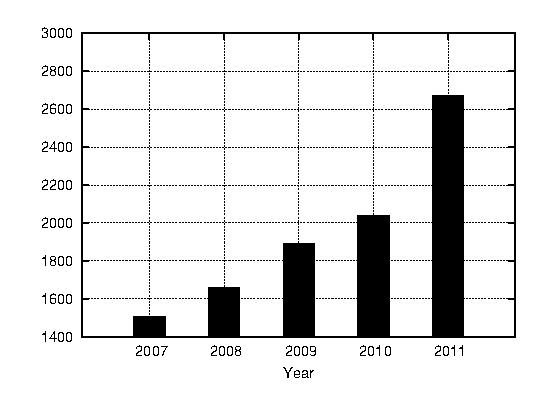
\includegraphics{OptimizationCFD.eps}}
\end{minipage}
\caption{Yearly number of publications on CFD-based optimization appearing in ScienceDirect.} 
\label{pubs.CFD}
\end{figure}

In order to demonstrate the increasing interest of the scientific community in CFD-based optimization, an internet-based literature survey was carried out using the search tool ``ScienceDirect'' (http://www.sciencedirect.com/). The search lemma was (Optimization $AND$ CFD) $OR$ (Optimization $AND$ Computational Fluid Dynamics).  This is obviously a non-exhaustive search; it is though good enough to show trends.  The steadily growing number of publications in the last five years, shown in fig.\ \ref{pubs.CFD}, reveals the growing interest in performing CFD-based optimization. Therefore, it is expected that the upgrades proposed in this thesis must be of interest to a continuously growing in size community of scientists, not necessarily restricted to those working in the field of turbomachines.     
 
A prerequisite for any shape optimization problem in fluid dynamics is the availability of a fast and reliable way to evaluate candidate solutions. This is achieved through the use of CFD (hence the term CFD-based optimization) methods that numerically solve the differential equations governing the fluid motion. Nowadays, thanks to the relatively cheap access to powerful computational means, the CFD tools have affordable CPU cost (depending on the case complexity) and, therefore, optimization methods based on them are flourishing. The strong dependence of the CFD-based optimizations on the computational resources becomes crucial in cases where several disciplines (ranging from structural analysis to manufacturing and economics, etc.) are used to evaluate the candidate solutions (multi-disciplinary optimization, MDO). The fact that the fluid dynamic, structural and economical objectives may be contradictory adds extra difficulty to the optimization procedure.           
 
An important part of any optimization project is the definition of the design variables. An optimization algorithm seeks the value set of the design variables which minimizes the user-defined cost function(s).  In CFD-based optimization, typical objectives are: maximization of lift,  minimization of drag,  maximization of efficiency, minimization of the deviation from given target (pressure, velocity, etc.) distributions, minimization of viscous or shock-induced losses or the cavitation index (in hydraulic turbomachines), etc. A single objective (single-objective optimization, SOO) or combinations of them can be used. Design-optimization problems with more than one objectives (multi-objective optimization, MOO) can be solved by concatenating the objectives into a single one, after multiplying them with appropriate weights. The difficulty of choosing the most appropriate weight values and the failure of this approach in non-convex optimization problems are the main weaknesses of this approach.  An improved way to solve MOO problems is the use of dominance-based methods that rank the candidate solutions according to Pareto dominance \footnote{Solution $a$ dominates solution $b$ if and only if $a$ is equal to $b$ with respect to all objectives but one and better than $b$ at least for one of them.}. These methods compute a set of optimal solutions forming the so-called front of non-dominated solutions or Pareto front, where none of them is dominated by any other front member with respect to all objectives.  Therefore, the choice of the optimal solution to be adopted relies upon additional criteria set by the decision-maker.  The design-optimization problem can, also, be subject to a number of constraints. In shape optimization related to fluid mechanics, constraints are imposed to geometrical quantities (for instance, thickness constraints so as to come up with manufacturable designs), structural quantities such as the maximum stress or deflection and/or flow-related quantities such as the minimum flow turning or the cavitation index, in turbomachines.          

In general, CFD-based shape optimization methods can be classified in two categories, namely direct and inverse ones. Direct methods \cite{phd_Giotis,phd_Kampolis,phd:papadim,kn:Emm2002,kn:Emm2004} solve the optimization problem through a number of trials that involve geometry generation, CFD-based flow predictions, computation of the objective function and, if necessary, its gradient computation.  On the contrary, inverse methods (should not be confused with inverse design problem \footnote{Inverse design problems use the deviation of the current from a desirable flow variable distribution as cost function.} that can be solved by direct methods) \cite{chav:95,ded:95} begin from a set of desirable flow field characteristics (such as those related to the boundary layer) and solve the inverse problem to define the geometry. The major advantage of inverse methods is their low cost and the fact that they don't need a starting geometry. On the other hand, their most noticeable drawback is the inability to handle constrained optimization problems. The inverse methods developed by LTT/NTUA are based on the Le Foll method \cite{lefoll} which is an integral method using a two-parametric boundary layer velocity profile. This method was extended to accommodate compressibility \cite{pap69}, surface curvature effects on the turbulent boundary layer development \cite{pap70} and boundary layer separation \cite{pap81} and was used for the design of both axial and radial turbomachines. Based on the above classification, this PhD thesis is dealing with direct design-optimization methods.  

Based on the way optimal solutions are sought, the optimization methods can be classified as deterministic and stochastic. In CFD-based optimization, deterministic methods were used first,  mainly due to their solid mathematical background and fast convergence, to locate optimal solutions with less trials. Deterministic methods require the computation of the gradient of the objective function with respect to the design variables. This limits the type of objective functions such a method might handle to those being differentiable. The cost of the gradient computation might become prohibitive if access to the evaluation software source code is not granted and computationally expensive finite-difference schemes must be employed. On the other hand, in MOO problems, they have difficulties to compute fronts of non-dominated solutions with a single run and they risk to be trapped into local minima.        

In the deterministic or gradient-based optimization methods used in fluid dynamics, the most important part is the gradient computation. The use of finite differences, as mentioned above, is not suitable since it requires, at least, as many flow analyses as the design variables. The use of adjoint techniques can reduce this cost to that of a single-equivalent flow solution irrespective of the number of design variables. Due to the need of significant investment in person-months (mathematical development and programming) required for the development of the adjoint methods and software, these were not used in CFD-based optimization since mid-$80's$ \cite{piron:84, kn:Jame88, kn:Jame94, kn:Jame95}.  The two variants of adjoint techniques, discrete and continuous, differ in the way the discretized adjoint equations are formed. The continuous adjoint method \cite{kn:Jame94, kn:Ander99,phd:papadim} processes the flow PDEs to derive the adjoint ones which are, then, discretized. On the other hand, in the discrete adjoint method, the adjoint equations result directly from the discretized flow equations, \cite{kn:Elliott96, anderson:99}. A more detailed presentation of adjoint methods used in fluid dynamic optimization can be found in \cite{phd:papadim}.        

On the other hand, stochastic optimization methods  do not suffer from the risk of getting trapped into local minima due to the probabilistic search they employ. The differentiability of the objective function is not required. An additional advantage of stochastic optimization methods, especially regarding industrial usage, is their ability to handle any problem, by merely accommodating the available evaluation software, without even having access to its source code. Their main drawback, though, is the need to evaluate a great number of candidate solutions before reaching the optimum. This may significantly increase the overall computational cost of the optimization procedure. This PhD thesis is dealing with stochastic optimization methods and, more precisely, EAs and aims at the reduction of computational cost. 

The use of EAs in CFD-based optimization was delayed until mid-$90's$, mainly due to their high computational cost. The first relevant works \cite{kn:Quag95,per:95,kn:Gala96} presented automated EA-based procedures for aerodynamic design-optimization problems. Soon after, emphasis was laid on the reduction of the cost of the overall optimization procedure, mainly by adapting the available variable representations and evolution operators. This continued with their hybridization with deterministic methods. For instance, in \cite{kn:Mar97} and \cite{kn:Fost97}, an EA was used to spot a good starting solution for a deterministic optimization method. In \cite{dennis:99}, EAs were hybridized with Sequential Quadratic Programming (SQP) for constrained shape optimization problems. Furthermore,  the use of distributed EAs \cite{kn:Door1997,kn:SefrThes}, surrogate evaluation models \cite{kn:Ratl98,kn:Gio99,kn:Gian1999,EBNK,phd_Kampolis}, hierarchical schemes \cite{kn:Eby1998,kn:Sef2000,knowles00mpaes_x41,Desid2003,phd_Kampolis} and concurrent evaluations on a multiprocessor platform \cite{kn:LeeH96,phd_Giotis,phd_Vera} have been proposed. Nowadays, the appeal of CFD optimization using EAs for industrial-scale engineering problems is growing due to the availability of powerful computational resources. This PhD thesis is dealing with the use of EAs for solving industrial-scale design-optimization problems in the fields of thermal and hydraulic turbomachines in acceptable (for industry) turn-around time.   


\begin{figure}[h!]
\begin{minipage}[b]{1\linewidth}
 \centering
 \resizebox*{!}{8 cm}{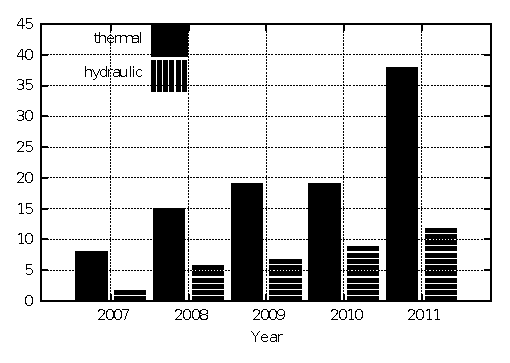
\includegraphics{hydrtherm_m.eps}}
\end{minipage}
\caption{Yearly number of recent publications which are relevant to the optimization of thermal and hydraulic turbomachines, in ScienceDirect.} 
\label{pubs.turbo}
\end{figure}
 

Regarding CFD-based optimization in the fields of thermal and hydraulic turbomachines, another internet-based literature survey was carried out, too. Search lemmata were: (a) optimization $AND$ thermal $AND$ turbomachines and (b) optimization $AND$ hydraulic $AND$ turbomachines. This survey reveals the steadily growing number of publications, in both turbomachinery areas, over the last five years, as shown in fig.\ \ref{pubs.turbo}. 

For instance, in the ASME 2011 Turbo Expo Conference, $24$ papers were related to the development and applications of EA-based optimization in the field of thermal turbomachines; some of them are not CFD-based. Most of them are handling a small number of design variables, $(N\!\leq\!15)$, and only three \cite{Georg2011,Marcel2011,Kevin2011} solve high-dimensional problems $(N\!>\!30)$. In \cite{Georg2011}, the application of an axisymmetric endwall contour for compressors is investigated. An EA-based optimization of the outer casing and the corresponding blade tip airfoil section of a typical gas turbine high-pressure compressor stage, with a high number of design variables ($N\!=\!38$), is presented. In \cite{Marcel2011}, the high-dimensional ($N\!=\!210$) constrained MOO of a fan stage, using EAs enhanced by metamodels, is presented. In \cite{Kevin2011}, an EA-based axisymmetric multi-disciplinary optimization approach for compressors is  applied to the design of a three-stage booster with $N\!=\!53$ design variables. Even though the aforementioned papers use a great number of design variables, they typically start from an almost optimal design and, therefore, are able to significantly restrict the design space per design variable. For instance,  \cite{Marcel2011} starts from a ``pre-optimized'' design and in \cite{Georg2011} the search space of each design variable is of the order of the tip clearance magnitude (very small). Note that the KBD method proposed by this thesis may efficiently deal with both high-dimensional ($N\!>\!300$) problems with extended search space per variable.      

In the IAHR 2010 conference, $5$ paper on the optimization of hydraulic turbomachines were presented. Three of them,  \cite{Raimunda2010,Kyriacou2010,Popa2010} used EAs. In \cite{Popa2010}, the weekly operation of a multipurpose
hydroelectric development, including a pumped storage plant was optimized using an EA. In \cite{Raimunda2010}, an optimization problem with two design variables, concerning the design of an axial compressor cascade using a MAEA was presented.  In \cite{Kyriacou2010}, the author of this thesis presented the solution of an optimization problem with $336$ design variables, concerning the design of a Francis hydraulic turbine. 


Research on the CFD-based optimization in the fields of thermal and hydraulic turbomachines was carried out in the Laboratory of Thermal Turbomachines (LTT/NTUA) and the Laboratory of Hydraulic Machines (LHM/NTUA) of NTUA. 
Concerning thermal turbomachines, a number of papers regarding both deterministic and stochastic optimization methods reflect the performed research at LTT/NTUA. Most of them are related to the optimal design of components of thermal turbomachines, such as compressor cascades, using a variety of optimization methods.  An indicative subset of them is mentioned below. The coupling of stochastic optimization methods with computational intelligence is presented in \cite{LTT_2_018,LTT_2_020,LTT_2_023}. There, the use of artificial neural networks as metamodels, in order to assist  EAs incorporating costly evaluation tools such as CFD codes, are proposed. In \cite{LTT_2_026}, the use of metamodels trained  on both responses and gradients is proposed and used in the inverse design of a 3D peripheral cascade. In \cite{LTT_2_031}, the hierarchical distributed MAEA is used for the viscous loss minimization of a compressor cascade. In \cite{LTT_2_040}, an asynchronous EA is demonstrated on the  design of a 2D compressor cascade and in \cite{LTT_2_045} a grid-enabled asynchronous MAEA is applied to the optimization of a 3D annular compressor cascade. In \cite{LTT_2_032}, an adjoint-based optimization method is proposed for the total pressure losses minimization in turbomachinery cascades.  In \cite{LTT_2_049},  the computation of the exact Hessian matrix of the objective function measuring total pressure losses in turbomachinery cascades is presented for use along with Newton methods. Multi-level strategies that combine adjoint-based methods with MAEAs for turbomachines are described in \cite{LTT_3_092}.


Concerning the CFD-based optimization in the field of hydraulic turbomachines, the work done at LHM/NTUA is related to: a) the design of optimal components of hydraulic machines, such as runner blades, and b) the optimal design of complete hydroelectric power plants and energy storage plants in combination with other forms of renewable energy generation sources, such as wind energy. Indicatively, in \cite{Anagno4}, the fast Lagrangian approach is incorporated into an EA to design an optimal Turgo turbine. The optimal sizing of a run-of-river small hydroelectric power plant utilizing an EA is described in \cite{Anagno3}. In \cite{Anagno5,Anagno6}, the optimization of pumped-storage systems for wind power plants is presented.

   

\section{EAs: Previous work at PCOpt/NTUA} % section headings are printed smaller than chapter names
\label{PRW}
An overview of previous PhD theses on EAs which were carried out by PCOpt/NTUA research group follows. 

Giotis' thesis \cite{phd_Giotis}, developed a generalized EA able to combine components of the two most widely used evolutionary optimization methods, namely Genetic Algorithms (GAs) and Evolutionary Strategies (ESs). In the same thesis or the corresponding papers \cite{kn:Emm2002,LTT_2_018,LTT_2_023}, the use of artificial neural networks as local metamodels, trained on previously evaluated candidate solutions, was proposed in order to reduce the computational burden. To reduce the wall clock time of the optimization, parallel evaluations of candidate solutions on a number of available processors, via the PVM protocol were used. The EASY optimization platform this thesis relies upon originated from Giotis' thesis \cite{phd_Giotis}.   

Karakasis' thesis \cite{phd_Karakasis}, further improved the EA efficiency by focusing on the optimal use of metamodels in MOO problems. One of the most important outcomes of this thesis was that the MAEA became equally efficient in both SOO and MOO, by overcoming problems related to: (a) the fact that, in MOO, the previously computed individuals, by the EA are spread along a front in the design space rather than clustered around the sought optimal solution and (b) the presence of outliers that require special treatment. Distributed EAs (DEAs) were programmed and validated, in order to increase the parallel efficiency of EAs and avoid stagnation during the early generations. Furthermore, the notion of Hierarchical EAs (HEAs) was introduced and this  was later refined in \cite{phd_Kampolis}.    In \cite{phd_Karakasis}, the use of a DEA on each level of the HEA associated with a different evaluation model was proposed.

In Kampolis' thesis \cite{phd_Kampolis}, the HEAs were upgraded by introducing hierarchical schemes other than those based on the combined use of low- and high-fidelity evaluation software. The latter made use of different parameterization schemes (coarse and fine) or different search methods allowing, thus, the combination of EAs with deterministic optimization methods. Finally, new artificial neural networks trained on both the objective functions values and their gradient were proposed, see also \cite{LTT_2_026}.          

Asouti's thesis \cite{phd_Vera}, proposed a different way to increase the parallel efficiency of EAs or MAEAs. This was achieved by introducing the so-called Asynchronous EAs (AEAs) or Asynchronous MAEAs (AMAEAs). By utilizing a number of strongly interconnected demes, according to a newly proposed topology, the asynchronous variants may circumvent the ``end of generation" synchronization barrier and, thus, uninterruptibly use all the available processors.     The proposed AEAs and AMAEAs are appropriate for heterogeneous multi-processor platforms. 


Georgopoulou's thesis \cite{phd_Chara}, proposed the so-called Metamodel-Assisted Memetic Algorithm (MAMA). Memetic Algorithms (MAs) are hybrid
methods that combine stochastic and deterministic search methods. The proposed MAMA combines the advantages of both MAEAs and MAs.
 
In a sixth PhD \cite{phd_eugene}, Kontoleontos also used the EASY platform to optimize energy production systems, such as
geothermal power plants and ground source heat pump systems.
 
 
\section{Thesis Outline} % section headings are printed smaller than chapter names
A short overview of the chapters of this PhD thesis follows:

Chapter $2$ presents the pre-existing algorithmic basis of this PhD. This includes the generalized EA with its evolution operators, the MAEA and the HEA.

Chapter $3$ is concerned with the first innovative method proposed in this PhD thesis, namely the Knowledge-Based Design (KBD) one. In the first part of this chapter, a short overview of KBS is presented. Then, the proposed KBD method is described in detail and used to perform the design of a 2D compressor cascade, in order to demonstrate its merits.

Chapter $4$ is dealing with EAs and MAEAs suitable to solve ill-posed optimization problems. This chapter starts by describing the features of ill-posed optimization problems. Then, the drop in EA efficiency when used to solve ill-posed problems is investigated. An innovative way to find new directions in the design space that, if used to redefine the design variables, would result in a better-posed problem that can be solved using EAs and MAEAs at lower computational cost is proposed.  New evolution operators, the so-called PCA-driven ones, are devised, in order to recover the aforementioned EA efficiency drop. Furthermore, the use of the importance information, resulting from the PCA is used to enhance metamodel's efficiency. Finally, the gain achieved using the proposed methods is quantified through a 2D compressor cascade design-optimization case.

In Chapter $5$, the methods proposed in Chapters 3 and 4 are used to solve large-scale industrial problems in the field of hydraulic turbomachines. The parameterization, grid generation and CFD tools used in this studies are presented. Quality metrics measuring each hydraulic turbine quality with respect to cavitation, blade loading and draft-tube coupling are introduced. Then, the optimization of a Francis turbine, performed in the context of a modernization/rehabilitation project, is used to demonstrate the merits of the KBD method, by comparing it with a conventional EA. Also, the optimization of a new type of hydraulic turbine, the so-called Hydromatrix$\circledR$, is carried out in order to demonstrate the gain expected from MAEAs using the proposed PCA-driven evolution operators.

Chapter $6$ is dedicated to the design-optimization of the compressor cascade installed at LTT/NTUA. This case is used to investigate the combined effects of using the PCA-driven evolution operators and the PCA-assisted metamodels,  proposed in Chapter $4$.

Finally, Chapter $7$ summarizes the conclusions drawn in this PhD thesis.      

%: ----------------------- HELP: references
% References can be links to figures, tables, sections, or references.
% For figures, tables, and text you define the target of the link with \label{XYZ}. Then you call cross-link with the command \ref{XYZ}, as above
% Citations are bound in a very similar way with \cite{XYZ}. You store your references in a BibTex file with a programme like BibDesk.


%%%%%%%% template for figures
%see fig \ref{A common glucose polymers}
%\figuremacro{EAvsPCA_zdt3}{A common glucose polymers}{The figure shows starch granules in potato cells, %taken from \href{http://molecularexpressions.com/micro/gallery/burgersnfries/burgersnfries4.html}{Molecular %Expressions}.}

%%: ----------------------- HELP: adding figures with macros
%% This template provides a very convenient way to add figures with minimal code.
%% \figuremacro{1}{2}{3}{4} calls up a series of commands formating your image.
%% 1 = name of the file without extension; PNG, JPEG is ok; GIF doesn't work
%% 2 = title of the figure AND the name of the label for cross-linking
%% 3 = caption text for the figure

%%: ----------------------- HELP: www links
%% You can also see above how, www links are placed
%% \href{http://www.something.net}{link text}

%\figuremacroW{EAvsPCA_zdt3}{Title}{Caption}{0.8}
%% variation of the above macro with a width setting
%% \figuremacroW{1}{2}{3}{4}
%% 1-3 as above
%% There you go. You already know the most important things.



	% background information
\chapter{Evolutionary Algorithms (EAs)} % top level followed by section, subsection

%: ----------------------- paths to graphics ------------------------

% change according to folder and file names
\ifpdf
    \graphicspath{{2/figures/PNG/}{2/figures/PDF/}{2/figures/}}
\else
    \graphicspath{{2/figures/EPS/}{2/figures/}}
\fi

%: ----------------------- contents from here ------------------------

%\begin{flushright}
%Life results from the non-random survival 
%\linebreak
%of randomly varying replicators.
%\linebreak
%Richard Dawkins 
%\end{flushright}
\section{Introduction - Overview of EAs}
\label{EAintro}
Several stochastic optimization methods have been inspired by and/or based on Darwin's theory of evolution on the origin of species \cite{Darwin}. Hereafter, the aforementioned methods along with their variants (there are plenty of them) will be referred to as Evolutionary Algorithms (EAs) \cite{HowToSolveIt}. The increasing power of modern multi-processor computational platforms and their availability at relatively low cost, combined with the inherent parallelization of population-based algorithms, suggest that EAs, combined with existing analysis tools, can be used as efficient industrial design tools. In our case, the analysis or problem-specific solution software is a Computational Fluid Dynamics (CFD) code. The cost of running the CFD code, quite often more than once per candidate solution (such as in case of a multi-point design) times the number of required trials determines the overall computational cost of the EA-based optimization.      

An EA is a generation-based, stochastic optimization method handling populations of individuals evolving from generation to generation. Each individual $\vec{x}$ represents a potential solution to the optimization problem in hand and must be evaluated to obtain a measure of its ``fitness'' or ``cost'', according to user-defined objective functions. In each generation, the EA selects the most fit among the previous generation members (the so-called ``parents'') and evolves them by applying evolution operators (recombination, mutation, etc.). The new population (``offspring'') is expected to fit better to the environment determined by the selected objective function(s).     

The first attempts to use EAs as problem solving techniques are dated back to mid-50's and can be found in separate works by Friedberg, Bremermann and Box. Friedberg \cite{Friedberg:1958:LMP:1662346.1662347, Friedberg:1959:LMP:1661923.1661930} presented an EA capable of creating a program to perform a given task; though quite premature by that time, this was in fact an ancestor of evolutionary programming (see below). During the same period of time, Bremermann \cite{Bremermann_62} was among the first to apply EAs to numerical (linear and convex) optimization problems including the solution of systems of nonlinear equations. Box proposed the use of EAs as a method for improving industrial processes and increasing productivity \cite{Box57a,BoDr98a}. By that time, these first attempts were treated with considerable skepticism. Soon after, several methods which initiated the three broad classes of EAs, namely evolutionary programming (EP), evolutionary strategies (ES) and genetic algorithms (GA), were brought to light.

EP was proposed by L. J. Fogel by mid-60's  \cite{fogel62,fogel64,fogel66}. EP was developed by considering machine learning tasks by means of finite-state machines (FSM\footnote{A finite-state machine (FSM) is a mathematical model used to design computer programs and digital logic circuits. FSM is an abstract machine that can be in one among a finite number of states.}). The optimization problem was  initially defined as evolving an algorithm (program) for predicting arbitrary time series.  In EP,  \cite{fogel66}, each offspring is created by randomly mutating each parent. The offspring with the best value is, then, retained to become a parent in the next generation. EP was successfully applied to problems in prediction identification, automatic control and pattern recognition. Until mid-80's, EP was confined to the FSM representation. In 1986 EP was extended to alternative representations including ordered lists for the travelling salesman problem and real-valued vectors for continuous function minimization. Later on, a self-adaptative EP \cite{fogel95} was proposed by including mutation variance in the evolution.

The first ES was proposed in 1965 by Rechenberg \cite{Rechenberg_1965} using discrete, binomially distributed mutations (centered at the parent's position) and just a single parent and a single offspring per generation. Later on, ES was further developed both by Rechenberg \cite{Rechenberg71} and Schwefel \cite{Schwefel75}, by introducing recombination and adaptive mutation \cite{Rechenberg71}. Using real-valued representation of the optimization variables, mutation is performed by adding a normally distributed random value to them. The introduction of recombination as an additional evolution operator for creating offspring, being impossible with just a single parent, led to the multi-membered ES. This is usually referred to as a $(\mu, \lambda)ES$, i.e.\ an ES with $\mu$ parents and $\lambda$ offspring. One of the most successful variances of ES is the covariance matrix adaptation ES (CMA-ES) \cite{hansen2003ecj}. In CMA-ES, the covariance matrix of the multivariate normal distribution, from which the candidate solutions are sampled, is updated during the evolution. CMA-ES was found to be particularly useful in solving non-separable optimization problems. \cite{hansen2001ecj,hansen1997ecj}.

In 1962, GAs were proposed by Holland \cite{Holland:1962:OLT:321127.321128,holland_1975} as an evolution emulating tool for aiding the understating of the underlying principles of adaptive systems \footnote{Systems that are capable to undergo self-modifications in response to their interactions with the environment which they must function in.}. In comparison to other contemporary researchers in the field of EAs, Holland focused differently and laid emphasis on the algorithmic nature of GAs in the sense that the reproduction and inheritance  mechanisms were based on operators, such as mutation, crossover and inversion, which are well known from genetics \footnote{Genetics is a branch of biology, the science of genes, heredity and the variation in living organisms.}. In addition, the representation of the evolving objects was made by using binary strings in direct analogy to the genetics genome. The binary string representation was one of the distinctions between ES and GA, considered as important at least in the early stages of their lives.  
 
Genetic Programming (GP) was proposed by Crammer in mid-80's \cite{cramer85} and was, then, improved by Koza \cite{Koz94} aiming at the automated design of computer programs with the ability to perform a given computational task. In GP, individuals (computer programs) are represented as tree structures \footnote{A tree structure can represent graphically the hierarchical nature of an object. Tree structures start from the so-called ``root" node, which is the highest in hierarchy. Lines connecting elements, to be referred to a nodes, are called ``branches". The lowest in hierarchy nodes are called ``end-nodes" or ``leaves". } where each node is given an operator function and each terminal node an operand. Representing programs in this way offers easy evaluation and makes the application of the evolution operators possible, in the sense that recombination can take place by exchanging nodes between the parents whereas mutation by replacing nodes at random. 
 

In PCOpt/NTUA, GA and ES are both represented by a generalised $(\mu,\lambda)EA$ \cite{phd_Giotis,phd_Karakasis,phd_Kampolis}, as described in section \ref{EASY_def}.  The $(\mu,\lambda)EA$ main characteristics are the population-based evolution and the fact that the inheritance of candidate solution features is based on both probabilistic criteria and decisions made upon a fitness or cost function, which quantifies the ability of each individual to survive in the user-defined environment. The evolution, from each generation to the next, fig.\ \ref{EA}, is carried out through the so-called evolution operators (parent selection, recombination, elitism and mutation). The generalised $(\mu,\lambda)EA$, which is used and enhanced in this PhD thesis, can be used as either a conventional ES or a conventional GA, by carefully adjusting the algorithmic settings and the optimization variable representation (binary or real coding).  

\begin{figure}[h!]
\begin{minipage}[b]{1\linewidth}
 \centering
 \resizebox*{!}{8 cm}{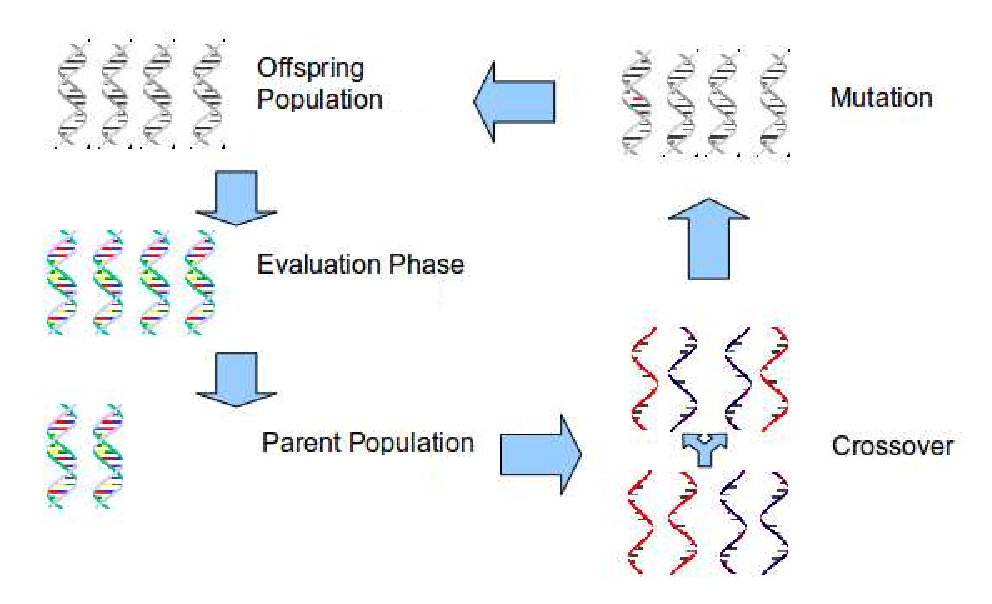
\includegraphics{EA.eps}}
\end{minipage}
\caption{Schematic representation of an EA. Each population is derived by the previous one via the application of evolution operators such as parent selection, crossover and mutation. Elitism is not shown here. } 
\label{EA}
\end{figure}



The three main advantages of EAs are their ability to (a) avoid being trapped into local optima and, thus, locate the global optimum, (b) compute Pareto fronts of optimal solutions in MOO problems, with a single run and (c) accommodate any ready-to-use analysis software without requiring access to its source code. The only prerequisite for carrying out an EA-based optimization is the availability of an appropriate evaluation software (even a commercial one, considered as a black–box tool within the optimization loop), objective functions and well defined design variables along with lower and upper bounds for each of them. However, the need to evaluate all individuals in each generation, so as to assign fitness or cost values to all of them, is the weak point of EAs, particularly if the evaluation of each candidate solution is computationally demanding. Optimization in aerodynamics or hydrodynamics which relies on expensive CFD software is a typical example.  This increases noticeably the optimization turn-around time and, often, makes the whole process non-affordable for industrial use. To overcome this weakness, several techniques have been proposed, \cite{LTT_2_020,Jin2002}. These  are classified in those reducing the optimization turn-around time by performing concurrent evaluations of the population members on a multi-processor platform and those reducing the number of evaluations needed to reach the optimal solution(s). These two techniques can certainly be combined. A first overview of these techniques is given below.  

A Parallel Evolutionary Algorithm (PEA) \cite{phd_Giotis,phd_Karakasis,phd_Kampolis,phd_Vera} is an EA adapted to take advantage of the availability of multi-processor systems, for reducing the optimization turn-around time. PEAs can be classified into single- and multi-population EAs. In a single-population or panmictic EA, each population member can, potentially, mate (be recombined) with any other. Standard way of parallelization is the concurrent evaluation scheme, with centralized selection and evolution (the so-called ``master-slave'' model). A multi-population EA handles partitioned individual subsets, according to a topology which often maps directly onto the parallel platform and employs decentralized evolution schemes; these can be further classified into distributed \cite{LTT_2_023,Herr1999,LTT_2_044} and cellular EAs \cite{alba_08,Nebro:2009p48}, depending on the subpopulations’ structure and granularity. 

All the aforementioned PEAs refer to synchronous EAs, in which the use of the multi-processor platform is restricted to the concurrent evaluation of candidate solutions, without altering the, generation-by-generation, sequential nature of evolution in EAs. This creates a synchronization barrier at the end of each generation; at this point, a number of processors may remain idle while waiting for the remaining generation members to be evaluated.  In order to minimize (practically eliminate) the idle time of processors, asynchronous EA (AEA) \cite{LTT_2_040,Alba2001} have been developed. The AEA proposed by PCOpt/NTUA overcomes the sequential nature of evolution by applying the evolution operators to a number of strongly interacting (overlapping) demes which may optimally use all the available processors.     

A metamodel-assisted EA (MAEA) employs low-cost surrogate evaluation models, i.e.\ the so-called ``metamodels'', as often as possible, during the optimization. This decreases substantially the number of calls to the computationally expensive, problem-specific evaluation code (such as the CFD software). Polynomial regression, artificial neural networks, Gaussian processes etc.\ have all been used as metamodels. Schemes based on different interactions between the metamodel and the problem-specific evaluation tool can be found in the literature \cite{KEANEbook,LTT_2_020,Jin2002,LTT_2_027}. MAEA implementations can be classified in two basic categories, depending on whether the metamodel(s) is/are trained separately from (off-line) or during (on-line) the evolution. Additionally, global (i.e.\ a single metamodel for the entire search space) or local (i.e.\ each of which being valid over a different part of the search space) metamodels can be used.

Additional reduction in the optimization turn-around time can be achieved by employing hierarchical EAs (HEAs) or MAEAs (HMAEAs)\cite{phd_Karakasis,phd_Kampolis,Herr1999,LTT_2_044, LTT_2_031,Lim2007}. These are built based on a small number of interconnected levels. On each level, different search methods, different evaluation software and/or different sets of design variables can be employed. One- or two-way inter-level communication schemes can be used. On levels employing EA-based search, a PEA or MAEA or both can optionally be used. Multi-level optimization algorithms can, generally, be classified as follows \cite{ParCFD}:

(a) \emph{Multi-level Evaluation,} where each level is associated with
a different evaluation software. The lower levels are responsible
for detecting promising solutions  at low CPU cost, through low-cost problem--specific evaluation models, and
delivering them to the higher level(s). There, evaluation models of
higher fidelity and CPU cost are employed and the immigrated
solutions are further refined. 

(b) \emph{Multi-level Search,} where each level is associated with a
different search technique. Stochastic methods, such as EAs, are
preferably used on the lower level(s) for the exploration of the
design space, leaving the refinement of promising solutions, often via gradient-based methods, on the higher level(s). Other
combinations of search tools are also possible. Memetic algorithms \cite{Krans2005,Ong2004,Ong2006,LTT_2_043,LTT_2_053,LTT_4_04} is a class of multi-level search that combines global and local search methods, where the latter aims at improving the quality of
promising solutions.


(c) \emph{Multi-level Parameterization,} where each level is
associated with a different set of design variables. On the lowest
level, a subproblem with just a few design variables is solved. On
the higher level(s), the problem dimension increases. The most detailed parameterization is used on the highest level.


%\figuremacroW{EA}{EA schematic representation }{Schematic representation of the EA. Each population is derived by the previous one via evolution operators, such as parent selection, crossover and mutation }{0.8}

\section{Optimization Problems - Definitions}
\label{OPt_def}
Any optimization problem with $M$ objectives (cast in vector $\vec{F}$) and $K$ constraints (cast in vector $\vec{C}$) can be formulated as:
\begin{align} 
   &min ~ \vec{F}(\vec{x})=(f_1(\vec{x}),f_2(\vec{x}),...,f_M(\vec{x}))\in \Re^{M} \nonumber \\
   &\mbox{subject to} ~ c_k(\vec{x})\leq d_k, ~~~~~ k =1,K
\label{OptimIN}
\end{align}
where $\vec{x}\in X \!\leq\! \Re^{N}$ is the design vector and $X$ the design space. If equality constraints $ c^*(x)=d^* $ are to be imposed, these can be transformed into inequality ones $ c(x)=\Vert c^*(x)-d^*\Vert \leq d $, where $ d \in \Re $ is an infinitessimally small number. If $M \!> \!1$, problem \ref{OptimIN} represents a multi-objective optimization (MOO) problem; in such a case, the notion of Pareto dominance \cite{Zitzler2000} is used to associate a scalar cost value to each individual, based on which an algorithm solving single-objective optimization (SOO) problems can be employed. In MOO problems, a single run of an EA is capable of delivering a Pareto front of non-dominated individuals, rather than a single ``optimal" solution, standing for an offset among the various objective functions. 

\subsection{Multi-Objective Optimization and EAs}
\label{MOOini}
In contrast to SOO where the scalar cost function, which determines the survival of candidate solutions from generation to generation, is derived directly from the objective function, a solver for MOO problems handles a vector of objectives. Therefore, in order to rely on the EA built for solving SOO problems, a technique to transform this vector to an appropriate scalar cost value is needed. In the literature, several techniques for handling this problem exist \cite{CoCo99,coe02,Miett99}. The most commonly used among them concatenate the $M$ objective functions into a scalar cost function, either by associating weights to each one of them or by accounting for the distance between the candidate solution and a user-defined ideal point in the objective space or, even, by using ranking techniques based on the notion of Pareto dominance (see below). In this PhD thesis, all MOO problems are handled using techniques relying on Pareto dominance criteria. Different implementations of Pareto dominance based techniques exist in the literature; among them, the most widely used ones are MOGA \footnote{Multi-objective Genetic Algorithm.} \cite{Fon93}, NPGA \footnote{Niched Pareto Genetic Algorithm.} \cite{horn94}, NSGA \footnote{Non-Dominated Sorting Genetic Algorithm.} \cite{Sri1995}, NSGA2 \cite{Deb00a}, SPEA \footnote{Strength Pareto Evolutionary Algorithm.}\cite{ZiTh98}, SPEA2 \cite{Zitz02}, PAES \footnote{Pareto Archived Evolution Strategy.} \cite{knowles99} and PESA \footnote{Pareto Envelope-based Selection Algorithm.} \cite{corne00}. The definition of Pareto dominance and Pareto optimality in minimization problems, which the aforementioned techniques rely on, follow:

\paragraph{Pareto Dominance:} Solution $\vec{x}_1$ dominates solution $\vec{x}_2$ ($\vec{x}_1\prec\vec{x}_2$) if and only if $\vec{F}(\vec{x}_1)$ is partially less than $\vec{F}(\vec{x}_2)$, i.e.
\begin{eqnarray}
    \vec{x}_1\prec\vec{x}_2 \Leftrightarrow (\forall i \in[1,M] :  f_i(\vec{x}_1) \leq f_i(\vec{x}_2))\wedge (\exists _i : f_i(\vec{x}_1) < f_i(\vec{x}_2))
   \label{pareto_eq} 
\end{eqnarray}

\paragraph{Pareto Optimality:} Solution  $\vec{x}_1 \in X$ is a Pareto optimal solution with respect to $X$ if and only if there is no $\vec{x} \in X$ that dominates $\vec{x}_1$, or 


\begin{eqnarray}
    \nexists\vec{x}:\vec{x}\prec\vec{x}_1, ~~~~ \vec{x},\vec{x}_1\in X \!\subseteq\! \Re^{N}
\end{eqnarray}
 
%\figuremacroW{Pareto2}{Pareto dominance}{Schematic representation of Pareto dominality. $\vec{x}_1$ is a Pareto optimal solution since it is not dominated by any other solution. Furthermore $\vec{x}_1$ itself dominates all individuals located in the grey box.}{0.5}

\begin{figure}[h!]
\begin{minipage}[b]{1\linewidth}
 \centering
 \resizebox*{!}{8 cm}{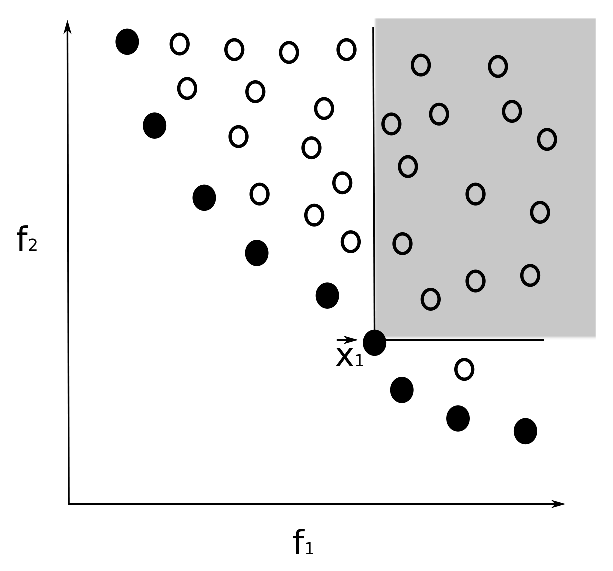
\includegraphics{Pareto2.eps}}
\end{minipage}
\caption{Schematic representation of Pareto dominance in a two-objective minimization problem ($min(f_1)$ and $min(f_2)$). $\vec{x}_1$ is a Pareto optimal solution since this is not dominated by any other solution. $\vec{x}_1$ dominates all individuals located in the grey box. All Pareto optimal solutions are marked with black circles.} 
\label{Pareto2}
\end{figure}


In fig.\ \ref{Pareto2}, a schematic representation of the Pareto optimality is shown. A minimization problem with two objective functions, $f_1$ and $f_2$, is considered. Black circles denote the front of non-dominated individuals whereas the empty circles denote dominated individuals. In the sake of clarity, the part of the objective space which is dominated by $\vec{x}_1$ is highlighted in grey. Individuals located in the grey area are dominated, at least, by $\vec{x}_1$. 

A detailed presentation of three techniques (SPEA, SPEA2 and NSGA2) used in this thesis follows in section \ref{MOO}.

\subsection{Constrained Optimization and EAs}
\label{COPini}
In engineering, almost all optimization problems are subject to constraints which split the design space into feasible and infeasible regions. EAs may handle constraints through (a) the use of penalty functions \cite{Deb00,morales98}, by assigning greater chances to survive to individuals satisfying the constraints \cite{powell93}, (b) the conversion of constraints into objectives \cite{surry95,surry97} and/or (c) the use of correction operators \cite{mich94}. A detailed survey on the subject can be found in \cite{mich96,coello02}. In the present thesis, penalty functions are used as presented in section \ref{COP}. 

\section{The Evolutionary Algorithm SYstem (EASY)}
\label{EASY_def}
EASY is a generic optimization platform which implements the $(\mu,\lambda)EA$, \cite{phd_Giotis,phd_Karakasis,phd_Kampolis,EASYsite}. EASY has been developed by PCOpt/NTUA and was used as the algorithmic basis for all techniques proposed in this thesis. EASY supports MAEAs using on- or off-line trained metamodels, various forms of multi-level optimization as described in section \ref{EAintro}, distributed and asynchronous search; it is also Grid/Cluster-computing enabled, based on the DRMAA library, \cite{phd_Liakopoulos}. A detailed analysis of the implemented $(\mu,\lambda)EA$, considered as the background optimization method in this thesis, follows.  


\subsection{The $(\mu,\lambda)$EA}
\label{MLEA}
Each generation, denoted by superscript $g$, of the $(\mu,\lambda)$EA is associated with three dynamically updated populations: the offspring $P_{\lambda}^g$ population with $\lambda$ offspring, the parent $P_{\mu}^g$ population containing $\mu$ parents and the elite $P_{e}^g$ population with $e$ elites. $P_{e}^g$ contains all or some of the currently best individuals. Depending on the design variables coding (binary, binary Gray or real), appropriate evolution operators are applied. 

The background $(\mu,\lambda)$EA in use, \cite{phd_Giotis}, comprises the following steps:
\begin{itemize}
\item[]{\bf Step 1:}  (Initialization) $g=0$, $P_{e}^{g-1}= \emptyset$ and $P_{\mu}^g= \emptyset$. All $P_{\lambda}^g$  members are initialized using a pseudo-random number generator, in accordance to the user-defined lower and upper bounds of each design variable. A number of user-defined individuals, such as existing sub-optimal solutions to the same problem or optimal solutions to similar problems, can optionally be included into the initial population. 
\item[]{\bf Step 2:}  (Evaluation) All individuals in $P_{\lambda}^g$ are evaluated using the problem-specific evaluation model. In all applications this thesis is dealing with, this is a CFD code. Later, when dealing with MAEAs, this will also be referred to as ``exact evaluation model'' to clearly distinguish it from evaluations (pre-evaluations) on cheaper surrogate models. The evaluation step is, always, considered to be time-consuming and yields vectors $\vec{F}(\vec{x}) \in \Re^{M} $ for each $\vec{x} \in P_{\lambda}^g$.
\item[]{\bf Step 3:}  (Cost assignment) For each $\vec{x} \in P_{\lambda}^g \cup P_{\mu}^g \cup P_{e}^{g-1}$, a scalar cost $\Phi(\vec{x})$ value is assigned based on $\vec{F}(\vec{x})$. In SOO, $\Phi(\vec{x}) \equiv F(\vec{x})$. In MOO, the techniques presented in section \ref{MOO} are employed. 
\item[]{\bf Step 4:}  (Elite selection) The $e^*$ non-dominated individuals (in a MOO problem) or the best one (SOO) in $P_{\lambda}^g \cup P_{e}^{g-1}$ are selected to enter $P_e^g$. If $e^*\!>\!e$, a thinning operator \cite{phd_Giotis} can be applied to remove the  $e^*\!-\!e$ excess individuals.     
\item[]{\bf Step 5:}  (Elitism) A few elite individuals, selected at random from $P_e^g$, replace the worst members of $P_{\lambda}^g$.  
\item[]{\bf Step 6:}  (Parent selection) The new parent population $P_{\mu}^{g}$ is selected from $P_{\mu}^{g-1}$ and $P_{\lambda}^g$ by taking into account the scalar cost values $\Phi$ computed in step 3 and the maximum allowed age  $\kappa$ (measured in generations) of each individual. Symbolically, $P_{\mu}^{g}=S(P_{\mu}^{g-1},P_{\lambda}^g,\kappa)$ 
\item[]{\bf Step 7:}  (Recombination and mutation) The next generation of the offspring population $P_{\lambda}^{g+1}$ is derived from 
$P_{\mu}^{g}$  by applying the recombination (or crossover) and mutation operators. Recombination $\mathcal{R}()$ is the process of combining the genotypes of $\rho$ parents to create an offspring (section \ref{evOps}). The recombination operator is used $\lambda$ times, with different sets of $\rho$ parents, randomly selected from $P_{\mu}^{g}$,  to create $\lambda$ new offspring. Next step is the application of the mutation operator. Mutation $\mathcal{M}()$ is a process which, with a small probability, randomly alters parts of the individual genotype. Symbolically, $P_{\lambda}^{g+1} = \mathcal{M}(\mathcal{R}(P_{\mu}^{g}))$ (section \ref{evOps}).
\item[]{\bf Step 8:}  (Stopping criterion) Unless any of the stopping criteria is met, return to $Step 2$.
\end{itemize}

The basic nomenclature of the ($\mu,\lambda$)EA is given in table \ref{GEA nomenclature}. 

\begin{table}[h!]
\centering
\begin{tabular}{lr} 
\hline
\hline
Number of design variables & N\\
Number of objectives & M\\
Number of constraints   & K\\
\hline
Candidate solution, design vector   & $\vec{x}=(x_1,...,x_N)$\\
Objective function &$f_i(\vec{x})$ \\
Vector of objective values (if M$>\!1$)  &$\vec{F}=(f_1(\vec{x}),...,f_M(\vec{x}))$\\
Constraint function &$c_i(\vec{x})$ \\
Vector of constraint values  & $\vec{C}=(c_1(\vec{x}),...,c_K(\vec{x}))$\\
Scalar cost value ($\Phi\!=\!f$ for M=1) & $\Phi$ \\
\hline
Number of offspring &   $\lambda$ 			\\
Number of parents &  $\mu$ 				\\
Number of elites &  $e$			\\
Maximum allowed age (in number of generations)&  $\kappa$			\\
Number of parents per offspring &  $\rho$			\\
\hline
\hline
\end{tabular}
\caption[GEA nomenclature]{Nomenclature of the ($\mu,\lambda$)EA.}
\label{GEA nomenclature} 
\end{table}
\FloatBarrier

\subsubsection{Evolution Operators}
\label{evOps}
The evolution operators employed in EASY are the parent selection,  recombination, mutation and  elitism. These are further discussed below: 
   
\paragraph{Parent Selection:}
The parent selection operator selects the members of $P_{\mu}^{g}$ from a set of already evaluated individuals. In EASY, based on the sixth step of the  algorithm presented in section \ref{MLEA}, this set is the union of $P_{\mu}^{g-1}$ and $P_{\lambda}^g$. The most common parent selection techniques  \cite{Back1996} are: 
\begin{itemize}
\item[]{\bf a) Proportional Selection:} Each member of $P_{\mu}^{g-1} \cup P_{\lambda}^g$ is given a probability to become a parent, which is inversely proportional to its cost value $\Phi$. Recall that a minimization problem is to be solved. The proportional selection is, practically, implemented via a roulette wheel. On the roulette wheel, each and every set member is given a slot, the angular size of which is proportional to its probability to become a parent. The roulette wheel is used $\mu$ times so as to create $\mu$ parents.  
\item[]{\bf b) Linear Ranking:} In linear ranking, the $P_{\mu}^{g-1} \cup P_{\lambda}^g$ members are sorted according to their $\Phi$ values. The probability of each one of them to become a parent depends linearly on its position in the corresponding list and not on the $\Phi$ values themselves.
\item[]{\bf c) Probabilistic Tournament Selection:}
In probabilistic tournament selection, \cite{goldberg1991}, a number of individuals are selected at random from the $P_{\mu}^{g-1} \cup P_{\lambda}^g$ set and, with a user-defined (typically high) probability, the best individual from this group is selected to become a parent. Otherwise, a randomly chosen one among the remaining individuals becomes parent. This is repeated $\mu$ times. In tournament selection, the most important user-defined parameters are the tournament size, i.e.\ how many individuals participate in each tournament and the probability of the best among them to be selected as parent. Typical values are: participation of $2$ or $3$ individuals in each tournament and $80\%$-$95\%$ probability to select the best among them.
\end{itemize}


\paragraph{Recombination:}
\label{RecombinationLabel}
Since the first appearance of EAs, numerous discussions about the advantages of employing the recombination operator can be found \cite{Schaffer87,Schaffer91,Navy92crossoveror}. In general, the purpose of recombination is to increase the probability of an offspring to become fitter than its parent(s). Recombination schemes can be classified depending on the design variables' coding. 

In EAs based on {\bf binary coding}, the recombination operator undertakes the exchange of pieces of binary strings encoding the design vector between the parents, in order to create an offspring. In EASY, the following recombination operators, which are appropriate for use with binary coding, exist:
\begin{itemize}
\item[]{\bf a) One-Point Recombination:} 
In the one-point binary recombination, with $\rho$ parents per offspring, the binary string is divided into $\rho \! - \! 1$ parts of equal length in binary digits. Then, $\rho$ parents are selected at random from the $P_{\mu}^{g}$ set and, using them, $(\rho \! - \! 1)$ pairs of parents are formed; all of them include the first parent. If the first parent is denoted by 1, the $(\rho \! - \! 1)$ pairs are: $(1,2),(1,3),...,(1,\rho)$. 
%The pairings take place serially between the lead parent (parent with higher $\Phi$) and the $i^{th} \in [1,\rho-1] $ one. 
For each one of the $(\rho \! - \! 1)$ pairs, a random integer $\mathcal{X}$ determines the corresponding crossover point. Each offspring is formed by combining the left part of the first parental string and the right part of the other parent, according to the aforementioned pairings. A three-parent example ($\rho=3$) is presented in fig.\ \ref{1px}.
\begin{figure}[h!]
\begin{minipage}[b]{1.0\linewidth}
 \centering
 \resizebox*{11cm}{!}{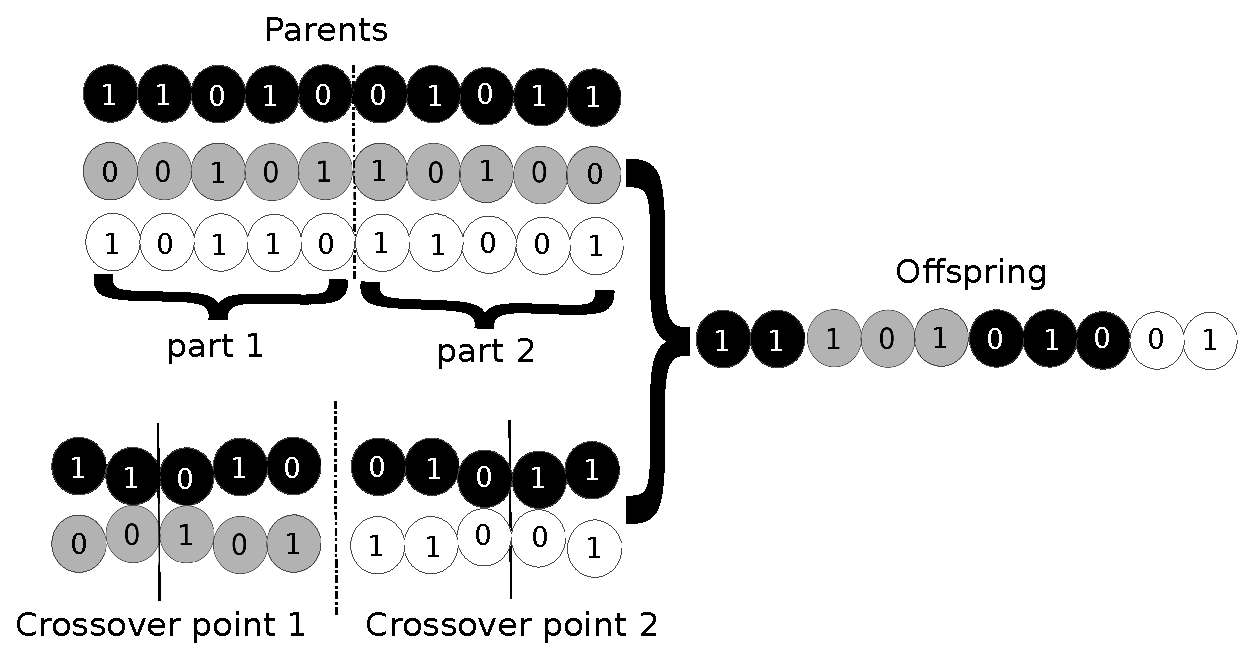
\includegraphics{onepointbinary.eps}}
\end{minipage}
\caption{One-point binary coding recombination with $\rho=3$. In this case, the chromosome is divided in two parts ($\rho-1 = 2$) and, then  a vertical cut per part is created at random.} 
\label{1px}
\end{figure}

\FloatBarrier
\item[]{\bf b) Two-Point Recombination:} This scheme is similar to its one-point counterpart, the only difference being that two crossover points $\mathcal{X}_1$ and $\mathcal{X}_2$ are used. A two-parent example is illustrated in fig.\ \ref{2px}.

\begin{figure}[h!]
\begin{minipage}[b]{1.0\linewidth}
 \centering
 \resizebox*{11cm}{!}{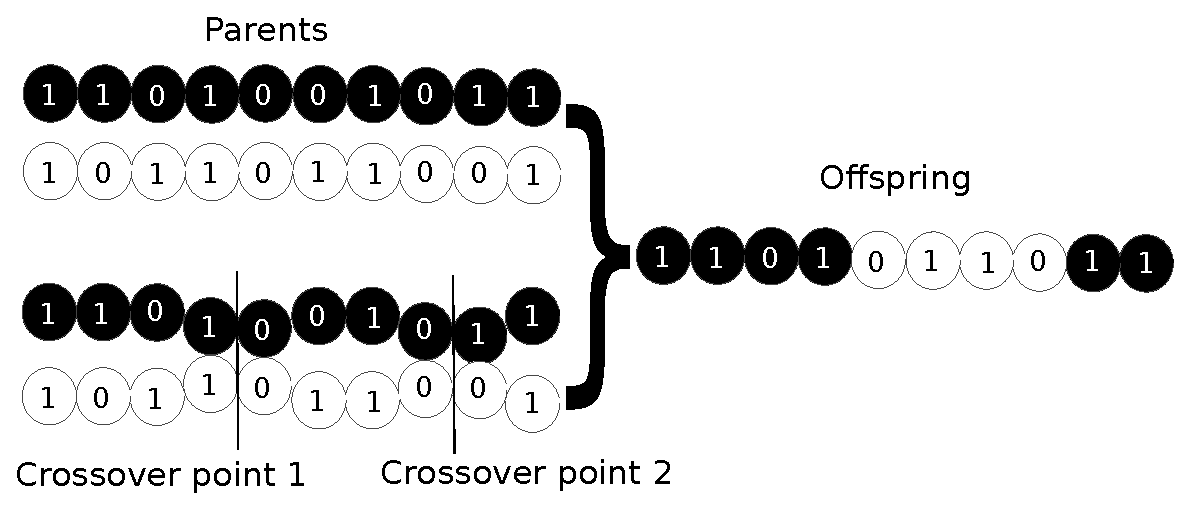
\includegraphics{twopointbinary.eps}}
\end{minipage}
\caption{Two-point binary coding recombination with $\rho=2$. In this simple case, the chromosome is handled as a whole ($\rho-1 = 1$) and two vertical cuts are created at random.} 
\label{2px}
\end{figure}

\FloatBarrier
\item[]{\bf c) One- or Two-Point Recombination per Design Variable:} Here, the aforementioned one- and two-point recombination schemes are separately applied to the parts  of the binary string that correspond to each design variable.  
\end{itemize}
  
Using {\bf real coding}, the recombination operator applies directly to the real-valued design variables. In EASY, this is carried out as follows:  

\begin{itemize}
\FloatBarrier
\item[]{\bf a) One- or Two-Point Recombination:} The one- and two-point recombination schemes, as described for binary coding, can be adapted to real coding by exchanging  pieces of the design vector $\vec{x}$ instead of pieces of binary strings. The randomly selected crossover variable is the only one to be affected by both parents according to a randomly generated weight $r$. A one-point, two-parent example is presented in fig.\ \ref{1pxreal}.

\begin{figure}[h!]
\begin{minipage}[b]{1.0\linewidth}
 \centering
 \resizebox*{11cm}{!}{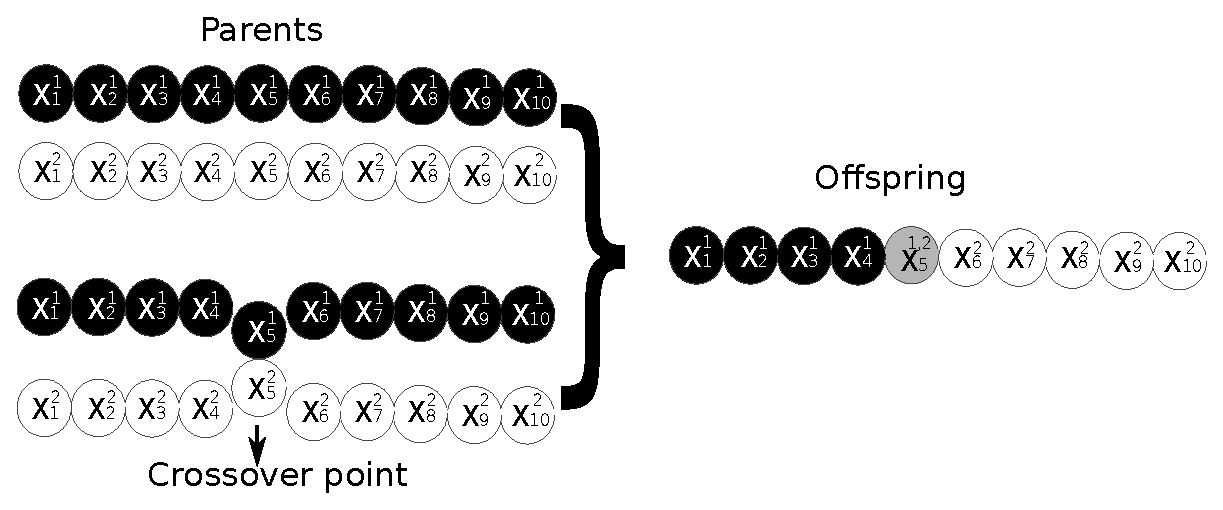
\includegraphics{pointreal.eps}}
\end{minipage}
\caption{One-point real coding recombination with $\rho=2$. The superscript and subscript denote the parent and the design variable respectively. The crossover variable (e.g. $5$) is selected at random. In the offspring, this variable is given by  $x_5^{1,2}=x_5^{1}+r(x_5^{2}-x_5^{1})$, where $r$ is a random number, uniformly distributed in $[0,1]$ ($r \in U(0,1)$).    
} 
\label{1pxreal}
\end{figure}
 
\FloatBarrier 
\item[]{\bf b) Discrete Recombination:} In discrete recombination with $\rho$ parents, each real-valued design variable in the offspring has $50\%$ probability to be copied either from the first parent $\vec{x}^1$ or any other  $\vec{x}^{~random}$, randomly chosen among the $\rho\!-\!1$ remaining ones. A three-parent example is presented in fig.\ \ref{disc}.

\begin{figure}[h!]
\begin{minipage}[b]{1.0\linewidth}
 \centering
 \resizebox*{11cm}{!}{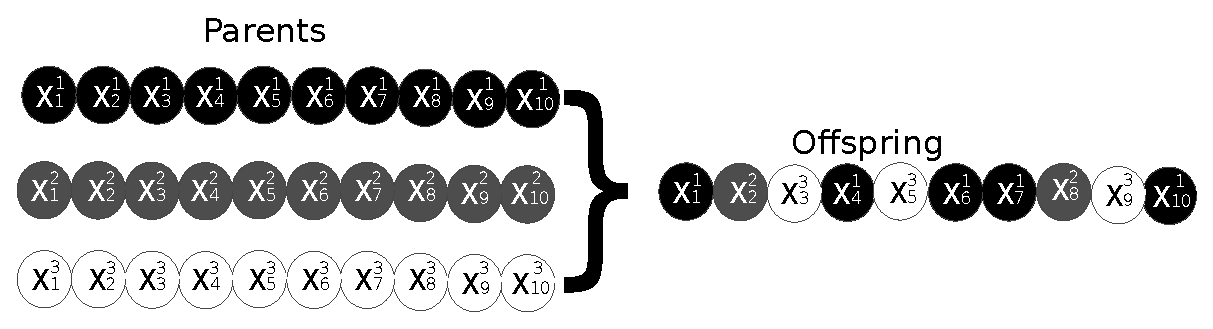
\includegraphics{discrete.eps}}
\end{minipage}
\caption{Discrete real coding recombination with $\rho=3$. $\vec{x^1}$ is the first parent.    
} 
\label{disc}
\end{figure}
    
\FloatBarrier    
\item[]{\bf c) Intermediate Recombination:}  In intermediate recombination, each component of  offspring $\vec{x}$ is a linear combination of the first parent $\vec{x}^1$ and $\vec{x}^{~random}$, which may be any other parent randomly chosen among the $\rho-1$ remaining ones. Thus,
\begin{eqnarray}
\nonumber
\vec{x}=\vec{x}^1+r(\vec{x}^{~random}-\vec{x}^1),~ r\in U[0,1]
\end{eqnarray}  
where $r \in U(0,1)$ means that $r$ is a random number, uniformly distributed in $[0,1]$. A different random number is generated for each design variable.

\FloatBarrier 
\item[]{\bf d) Simulated Binary Crossover:} The so-called simulated binary crossover (SBX) \cite{SBX1} aims at recreating the one-point binary recombination by replicating its (a) average property \footnote{The average of the decoded variable values is the same
before and after the crossover operation.} and (b) spread factor property\footnote{The spread factor ($\beta$) is defined as the ratio of the spread of offspring to that of parents. Contracting, expanding or stationary recombination correspond to $\beta \! <\!1$, $\beta\! >\!1$ or $\beta \!=\!1$ respectively. The spread factor property states that the occurrence of spread factor $\beta \! \approx \! 1$ is more likely than any other $\beta$ value. } \cite{SBX1}. The offspring $\vec{x}$ is generated based on the formulas
\begin{eqnarray}
	\vec{x}={\left\{ 
	\begin{array}{ll}
    \vec{\overline{x}} - \frac{\beta}{2} (\vec{x}^{~random}-\vec{x}^1)~~,\mbox{$r < 0.5$}\\
	\vec{\overline{x}} + \frac{\beta}{2} (\vec{x}^{~random}-\vec{x}^1)~~,\mbox{$r \geq 0.5$}
    \end{array} \right. }
    \label{sbxx}
\end{eqnarray}  
where $r\in U[0,1]$, $\vec{x}^1$ the first parent, $\vec{x}^{~random}$ is randomly selected among the $\rho-1$ remaining parents, $\vec{\overline{x}}$ is the middle point between $\vec{x}^{1}$ and $\vec{x}^{~random}$ and the spread factor $\beta$ is defined by
\begin{eqnarray}
	\beta={\left\{ 
	\begin{array}{ll}
    (2r)^{n}~~~~~~,\mbox{$r \leq 0.5$}\\
	\left(\frac{1}{2r}\right)^{n+2}~~,\mbox{$r > 0.5$}
    \end{array} \right. }
    \label{betasbx}
\end{eqnarray}

Given that $r  \! \in  \! U[0,1]$, the probability distribution of $\beta$  can be plotted for various values of $n$ based on eq.\ \ref{betasbx} (fig.\ \ref{sbx}, left). Based on the $\beta$ probability distribution and eq.\ \ref{sbxx}, the probability distribution of offspring appearance on the design space as a function of $n$ can be plotted (fig.\ \ref{sbx}, right for a 1D problem and fig.\ \ref{sbx2} for a 2D problem). In general, higher $n$ values increase the probability of $\beta \approx 1$, which in turn increases the probability of creating near-parent offspring (spread factor property). This, together with the symmetrical offspring probability distribution with respect to $\vec{\overline{x}}$ (average property), show that SBX may in fact simulate the one-point binary crossover.    

\begin{figure}[h!]
\begin{minipage}[b]{0.5\linewidth}
 \centering
 \resizebox*{7cm}{!}{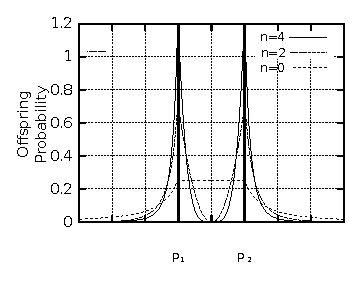
\includegraphics{SBXparents.eps}}
\end{minipage}
\begin{minipage}[b]{0.5\linewidth}
 \centering
 \resizebox*{7cm}{!}{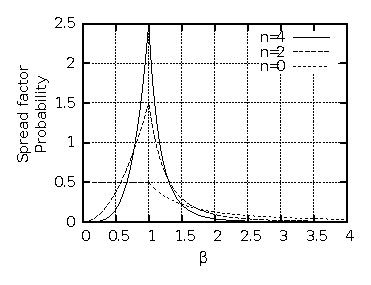
\includegraphics{SBX.eps}}
\end{minipage}
\caption{The offspring probability distribution of a 1D problem using SBX, with various values of $n$, is plotted as a function of the parents $P_1$ and $P_2$ (left). The corresponding probability distributions of $\beta$ are plotted on the right. Increasing $n$ leads to higher probability of $\beta \approx 1$.  }
\label{sbx}
\end{figure}

\begin{figure}[h!]
\begin{minipage}[b]{1\linewidth}
 \centering
 \resizebox*{13cm}{!}{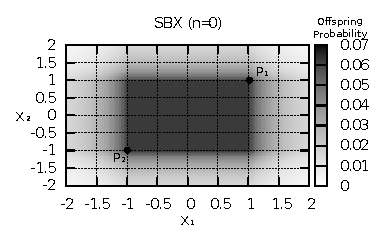
\includegraphics{SBX3dparents0.eps}}
\end{minipage}
\begin{minipage}[b]{1\linewidth}
 \centering
 \resizebox*{13cm}{!}{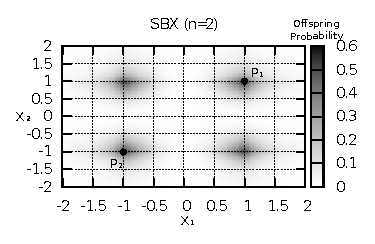
\includegraphics{SBX3dparents2.eps}}
\end{minipage}
\caption{The offspring probability distribution in a 2D optimization problem using SBX recombination for $n\!=\!0$ (top) and $n\!=\!2$ (bottom) is presented. The recombination uses two parents, namely $P_1(1,1)$ and $P_2(-1,-1)$.}
\label{sbx2}
\end{figure}
\end{itemize}

%\FloatBarrier   
\paragraph{Mutation:}
In EAs, the role of mutation is to introduce and preserve diversity in the population. Thus, mutation prevents the population from becoming prematurely homogenized, in which case slow or stagnated evolution may occur. Mutation is applied to each offspring generated using the recombination operator, subject to a small mutation probability $P_m$. From the implementation viewpoint, mutation depends on whether binary or real coding is used.

In EAs based on {\bf binary coding}, mutation is applied to each and every bit of the binary string. Each bit can be inverted (flip\footnote{Bit flip is a state switch, from 0 to 1, or vice-versa.}), with a probability $P_m$.      

\begin{figure}[h!]
\begin{minipage}[b]{1\linewidth}
 \centering
 \resizebox*{10cm}{!}{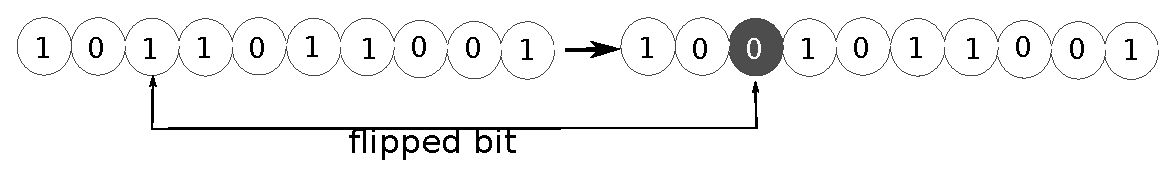
\includegraphics{mut.eps}}
\end{minipage}
\caption{Binary coding mutation.}
\label{binarymut}
\end{figure}

In {\bf real coded EAs},  mutation is applied to each real-valued component of $\vec{x}$, 

\begin{eqnarray}
	\vec{x}_m={\left\{ 
	\begin{array}{ll}
    \vec{x}~~~~~~~~~~,\mbox{$P_m > r$}\\
	M(\vec{x},D)~,\mbox{$P_m \leq r$}
    \end{array} \right. }
    \label{}
\end{eqnarray}
where $r\in U[0,1]$ seeded separately for each member of $\vec{x}$ and

\begin{eqnarray}
	M(\vec{x},D)={\left\{ 
	\begin{array}{ll}
    \vec{x}+D(g,\vec{U}-\vec{x})~,\mbox{$r_1 > 0.5$}\\
	\vec{x}-D(g,\vec{x}-\vec{L})~,\mbox{$r_1 \leq 0.5$}
    \end{array} \right. }
    \label{}
\end{eqnarray}
where $r_1\in U[0,1]$, $\vec{U}$ and $\vec{L}$ are the vectors of upper and lower bounds of $\vec{x}$ respectively and  

\begin{eqnarray}
   D(g,y) = y r_2 (1-g/g_{max})^{0.2}
\end{eqnarray}
where $g_{max}$ the number of maximum generations and $r_2\in U[0,1]$. Alternatively, the termination criterion can be based on the number of evaluations, so $g/g_{max}$ must be replaced with $Ev/Ev_{max}$, where $Ev$ is the evaluation counter and $Ev_{max}$ the maximum allowed number of evaluations.  

%\begin{eqnarray}
%	\vec{\sigma}=\frac{min(\mid \vec{x}-\vec{UB}\mid,\mid \vec{x}- \vec{LB}\mid)}{3} * (1-\frac{g}{g_{max}})^p
%	\label{sigmamut} 
%\end{eqnarray}
%where $\vec{UB}$ and $\vec{LB}$ the vectors of upper and lower bounds for the design variables respectively. $g$ the current generation and $g_{max}$ the maximum allowed generations.$p \simeq 0.2$.

%The first part of the eq.\ref{sigmamut} ensures that the mutated individual will respect the design variable bounds and the second part reduces exponentially eith $p$ the magnitude of $\vec{\sigma}$ as the generations advance.

%\begin{figure}[h!]
%\begin{minipage}[b]{0.5\linewidth}
% \centering
% \resizebox*{7cm}{!}{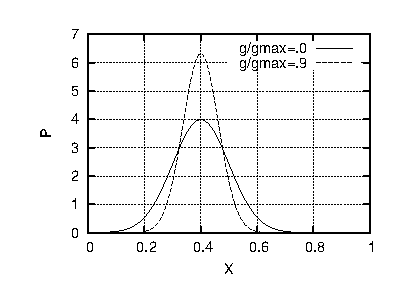
\includegraphics{Mut_1d.eps}}
%\end{minipage}
%\begin{minipage}[b]{0.5\linewidth}
% \centering
% \resizebox*{8cm}{!}{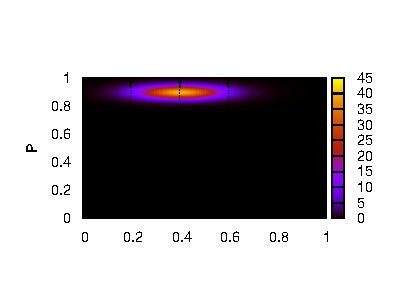
\includegraphics{Mut_2d.eps}}
%\end{minipage}
%\label{realmut}
%\caption{Examples of mutant probability distributions for one design variable left $x=0.4$ and two design variable right $\vec{x}=(0.4,0.9)$. For both cases $\vec{LB}=0$ and $\vec{UB}=1$.}
%\end{figure}

\paragraph{Elitism:}
In EAs, the purpose of elitism is to guarantee a monotonously improving course of evolution \cite{Back1996}. In EASY, a separate population $P_e^g$ is maintained and updated accordingly at the end of each generation (step 4 of the ($\mu,\lambda$)EA, section \ref{MLEA}). Elitism implies that a user-specified number of elite individuals replace the worst members of the offspring population $P^g_{\lambda}$, prior to the application of the parent selection operator.
  
\subsection{Solving MOO Problems with EASY}
\label{MOO}
As mentioned in section \ref{MOOini}, in MOO problems, a technique that transforms $\vec{F}$ into a scalar cost function $\Phi$ is required. Symbolically,

\begin{eqnarray}
    \Phi(\vec{x})=\Phi(\vec{F}(\vec{x})) :\Re ^M \rightarrow \Re ^1 
	\label{MOOeq}
\end{eqnarray}
The SPEA, SPEA2 and NSGA2 techniques, which are available in EASY, are presented below.

\paragraph{SPEA:}
SPEA was proposed by Zitzler and Thiele \cite{ZiTh98} in 1998 as a MOO cost assignment technique based on Pareto dominance. In SPEA, $\Phi(\vec{x})$ is computed in two steps as follows:
\begin{itemize}

\item[]{\bf Step 1:}  (Strength Computation) The strength of each member of the population $P=P_{\lambda}^g \cup P_{\mu}^g \cup P_{e}^{g-1}$ is computed. The strength of individual $i$ ($S_i$) is defined as the sum of the population members which are dominated  by $i$, divided by the population size, namely 

\begin{eqnarray}
	S_i = \frac{\sum(j : j \in P \wedge i \prec j)} {\sum P}, ~~ \forall i \in P =P_{\lambda}^g \cup P_{\mu}^g \cup P_{e}^{g-1}  
\end{eqnarray}

\item[]{\bf Step 2:}  (Cost Computation) The cost value $\Phi$ for each population member is computed as the sum of strengths of the population members which dominate it,

\begin{eqnarray}
	\Phi_i = \sum _{j \in P \wedge i \prec j}S_j
\end{eqnarray}
\end{itemize}
  
 
\paragraph{SPEA2:}
SPEA2 \cite{Zitz02} is an enhanced variant of SPEA which additionally incorporates density information. A nearest neighbour density estimation technique which allows a more precise guidance of the search process is incorporated, thus improving, compared to SPEA, the distribution of individuals along the Pareto front. 

SPEA2 performs three steps to compute $\Phi$. These steps are:

\begin{itemize}
\item[]{\bf Step 1:}  (Strength Computation) As in SPEA.

\item[]{\bf Step 2:}  (Density Computation) For each population member, the density metric $D_i$ is calculated  as a function of its distance from its closest neighbour in the objective space $d_i$,

\begin{eqnarray}
	D_i = \frac{1} {d_i+2} 
\end{eqnarray}
where
\begin{eqnarray}
	\nonumber
	d_i= min (\parallel \vec{F_i} - \vec{F_k} \parallel), ~ k \in P  
\end{eqnarray}


\item[]{\bf Step 3:}  (Cost Computation) The cost values for all population members are calculated as the sum of the raw cost $R_i$ and the density metric, $D_i$,

\begin{eqnarray}
	\Phi_i = R_i+D_i
\label{SPEAIIeq}
\end{eqnarray}
Here, $R_i$ is the sum of the individual strengths of the population members which dominate it, namely
  
\begin{eqnarray}
	\nonumber
	R_i=\sum _{j \in P \wedge i \prec j}S_j 
\end{eqnarray}  
\end{itemize}

\paragraph{NSGA2:} 
NSGA2 \cite{Deb00a} is an improved variant of NSGA \cite{Sri1995} addressing the high computational complexity of non-dominated sorting, the lack of elitism and the need for specifying the sharing parameter of the initial algorithm. A modified variant of NSGA2 is available in EASY. As proposed in \cite{Deb00a}, instead of computing $\Phi$ values, NSGA2 relies upon sorting the individuals according to Pareto dominance and density criteria. The modified variant of NSGA2 used in this PhD thesis includes the following steps:    


\begin{itemize}
\item[]{\bf Step 1:}  (Front Ranking) All members of the population are classified in fronts with decreasing Pareto dominance.  
\begin{itemize}
\item[]{\bf Step 1-a:}  (Initialization) Initialize the front counter $i=0$ and the auxiliary set $S=P_{\lambda}^g \cup P_{\mu}^g \cup P_{e}^{g-1}$.

\item[]{\bf Step 1-b:}  (Find non-dominated members of $S$) Locate the non-dominated members of $S$ and copy them to $\mathcal{F}_i$. 

\item[]{\bf Step 1-c:}  (Update) Update $S=S-\mathcal{F}_i$ % http://www.mathwords.com/s/set_subtraction.htm
and $i=i+1$. if $S\neq\O$ go to Step 1-b; else, set the number of fronts $N_F$ equal to $i-1$.
\end{itemize}
\item[]{\bf Step 2:}  (Density Computation) For each member $j \in \mathcal{F}_i$, the density metric $d_j$, which is equal to the average side-length of the cuboid defined by its neighbouring individuals in $\mathcal{F}_i$, is computed. This procedure is repeated for all fronts $i$ and all individuals are given a density metric value.

\item[]{\bf Step 3:}  (Cost Computation) Based on the density metric (calculated in Step 2) and front $i$ (calculated at Step 1) which each individual belongs to, a scalar $\Phi$ is assigned to each individual as follows,
\begin{itemize}
\item[]{\bf Step 3-a:}  (Initialization) Set $i=0$ and $\Phi_b=1.0$.
\item[]{\bf Step 3-b:}  (Computation of $\Phi$) For each member $j \in \mathcal{F}_i$, $\Phi$ is calculated as

\begin{eqnarray}
	\nonumber
	\Phi_j= \Phi_b(1+\frac{d_{max}-d_j}{d_{max}}) 
\end{eqnarray} 
where $d_{max}$ is the maximum of all $d_k$ $\forall k \in \mathcal{F}_i$   
\item[]{\bf Step 3-c:}  (Update) Update $\Phi_b=1.1max(\Phi_j)$ and $i=i+1$. If $i \leq N_F$ return to Step 3-b, otherwise stop. 
\end{itemize}
\end{itemize}

\subsection{Constraints' Handling in EASY}
\label{COP}
In EASY, penalty functions are used to handle constrained optimization problems (COP), see section \ref{OPt_def}. Penalty terms, proportional to the magnitude of the constraint violation, are added to the cost function. According to eq.\ \ref{penal2}, for each constraint, a ``nominal threshold'' $d_k$ is defined as the maximum possible constraint function value allowed by the optimization problem. Furthermore, a ``relaxed'' threshold $d_k^* > d_k$ is introduced. Once an individual violates the relaxed threshold of one of the constraints ($c_k \! > \! d_k^*$), death penalty ($\Phi \! = \! \infty$) is given to it. If the individual violates one or more of the constraints ($d_k \! < \! c_k \! < \! d_k^*$) without exceeding any of the relaxed threshold values, its cost value $\Phi$ is penalized as follows:

\begin{eqnarray}
	\Phi(\vec{x})=\Phi(\vec{x})+ \prod _{k=1}^K{\left\{ 				\begin{array}{ll}
    exp(a_k\frac{c_k(x)-d_k}{d_k^* -d_k}) & ~~,c_k(x)>d_k\\
    1 & ~~,c_k(x)\leq d_k\end{array} \right. }
    \label{penal2}
\end{eqnarray}  
where the user-defined set of coefficient values in $\vec{a}$ control the penalization intensity.

%\begin{figure}[h!]
%\begin{minipage}[b]{1.0\linewidth}
% \centering
% \resizebox*{10cm}{!}{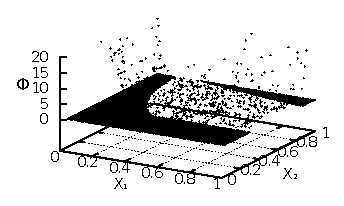
\includegraphics{fit_new.eps}}
%\end{minipage}
%\caption{$\Phi$ plot for 1000 randomly chosen individuals over the 2d design space of a two-objective constrained optimization problem (fig.\ref{case}) using the proposed penalization formulation (eq.\ref{penal2}).}
%\label{fit2}
%\end{figure}
 

\subsection{Metamodel-Assisted Evolutionary Algorithm (MAEA)}
\label{MAEApar}
Due to the use of costly evaluation models (such as the CFD software to numerically predict flows in or around complex 3D geometries), solving engineering optimization problems by means of EAs may become very computationally demanding. The extensive smart use of low-cost surrogate evaluation models (often referred to as ``metamodels'') during the optimization decreases substantially the number of calls to the computationally expensive, problem-specific evaluation code (CFD). This makes EAs a viable tool which can routinely be used to solve large-scale industrial optimization problems, in affordable wall clock time. Literature surveys on the use of metamodels within EAs can be found in papers \cite{LTT_2_020,Jin2002,LTT_2_027,EBNK} or books \cite{KEANEbook}.


Polynomial regression, artificial neural networks, Gaussian processes etc.\ have all been used as metamodels. The existing MAEAs differ since they apply different interactions between the metamodel and the problem-specific evaluation models. Hereafter, all of them will be referred to as MAEAs. In this thesis, on-line trained metamodels are used \cite{LTT_2_018,LTT_2_020,LTT_2_029}. 
 
In on-line trained metamodels, for all but the first few generations, the metamodels are used to pre-evaluate the current population. Based on the outcome of approximate pre-evaluations (Inexact Pre-Evaluations, IPE), the few most promising individuals are identified and these solely undergo evaluation with the problem-specific evaluation model to compute their ``exact''  objective function value(s), before proceeding to the next generation. The $(\mu,\lambda)$ MAEA is sketched in fig.\ \ref{MAEA}.


\begin{figure}[h!]
\centering
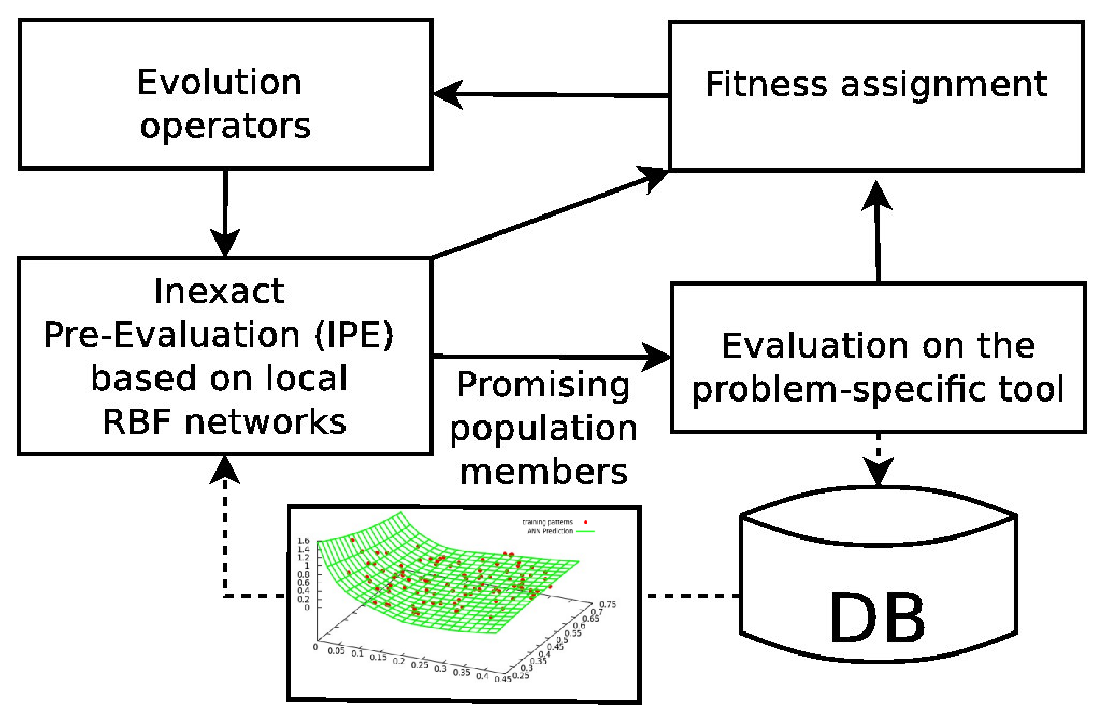
\includegraphics[width=90mm]{MAEA.eps} 
\caption{The $(\mu,\lambda)$MAEA using on-line trained metamodels. The loop corresponds to a single EA generation. The IPE phase, within the EA--based search, is described in \cite{LTT_2_018,LTT_2_020,LTT_2_029}. }
\label{MAEA}
\end{figure}


\paragraph{Radial Basis Function (RBF) Networks:}
In this PhD thesis, RBF networks are used as metamodels. Nevertheless, the new methods proposed in the next chapters could be combined with any other type of metamodels. RBF networks are artificial neural networks (ANNs) \cite{Hayk1999} with three neuron layers, (input, hidden and output) as shown in fig.\ \ref{rbf1}. Signals propagate through the network in the forward direction, from the input to the output layer, by performing a nonlinear mapping (eq.\ \ref{RBFa}) followed by a linear one. This mapping introduces weight coefficients $w_l$ that must be computed during the network training on a number of available patterns. An RBF network to be used within a MAEA should have $N$ input units, i.e.\ as many as the  design variables. The hidden layer includes $L$ nodes, associated with the so–called RBF centers $c^l$. At each hidden neuron, a nonlinear mapping of the input signals to a single value is performed using the radial-basis activation function $G:\Re^N \rightarrow \Re$, acting on the distance of input $\vec{x}$ (eq.\ \ref{RBFa}) from the corresponding center $\vec{c^l} \in \Re^N$.  In the present thesis, the Gaussian activation, 

\begin{eqnarray}
	G(u,r)=exp(\frac{-u^2}{r^2})
	\label{RBFa}
\end{eqnarray}  
where $u=\Vert x-c^l \Vert_2$ the distance from the corresponding $l^{th}$ RBF center, is used.

\begin{figure}[h!]
\centering
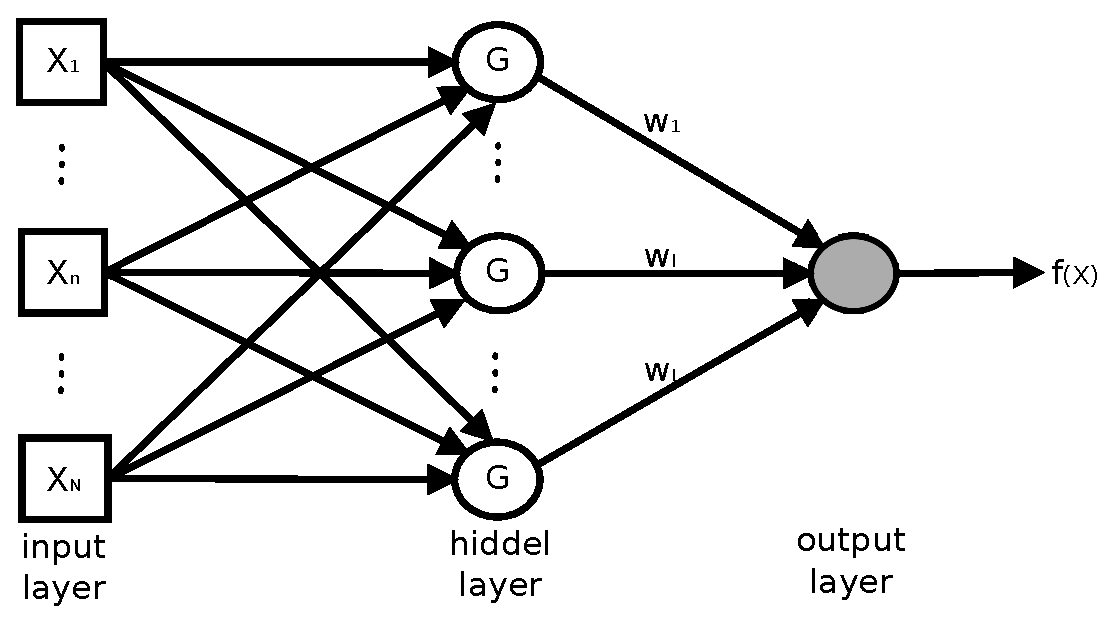
\includegraphics[width=90mm]{RBF.eps} 
\caption{Radial basis function (RBF) network.}
\label{rbf1}
\end{figure}

The radii or widths r values may considerably affect the prediction abilities of the network; these are computed using heuristics, \cite{Hayk1999}. The output layer includes as many nodes as the expected network responses. The single response we are dealing with is expressed by the sum of the weighted output signals from the hidden neurons, as follows             
\begin{eqnarray}
	f(x)=\sum _1^K w_i G(u(x_i),r)
\label{response}
\end{eqnarray}  

If the number of hidden nodes ($K$) is equal to the number of training patterns ($T$), the choice of the $RBF$ centers is straightforward, i.e.\
$\vec{c}^{(t)}\!\equiv\!\vec{x}^{(t)}$, $t\!\in\![1,T]$, ensuring
that the $T$ samples are exactly interpolated. 
In this case, the network training requires the solution of the $T\!\times\!T$ symmetric linear system of equations, 
%
\begin{equation}
    \sum_{t=1}^{T} w_t G(\|\vec{x}^{(t)}-\vec{c}^{(t)}\|_2)=
    \zeta^{(t)}
    \nonumber
\end{equation}

A common way to increase the network's generalization \cite{Pog1990, Tik76, Tik95} is by using a smaller number of appropriately selected hidden nodes than the training patterns, i.e.\ by selecting $K\!<\!T$. 
In such a case, the selection of the $RBF$ centers is not as straightforward as in the aforementioned case and is of great importance because 
it strongly affects the prediction ability of the network. 
In \cite{LTT_2_029}, a selection scheme for the $RBF$ centers based on 
self-organizing maps ($SOMs$), \cite{Fri94a, Hayk1999} was proposed. 
This practically consists of a two level learning process, namely the unsupervised and  supervised ones.
During the unsupervised learning, through their standard processes: 
competition, cooperation and adaptation, $SOMs$  classify the training 
patterns into $K$ clusters.  
Each cluster gives a single $RBF$ center $\vec{c}^{(k)}$, considered to be representative of the cluster as a whole. The corresponding radius $r_k$ is computed using heuristics based on distances between the centers, \cite{Karay1997, LTT_2_029, Hayk1999, BenArc02}.
During the supervised learning, the synaptic weights are computed by minimizing the approximation error of the $RBF$ network over the training set, while considering smoothness requirements.
%
%\begin{figure}
%    \centering
%    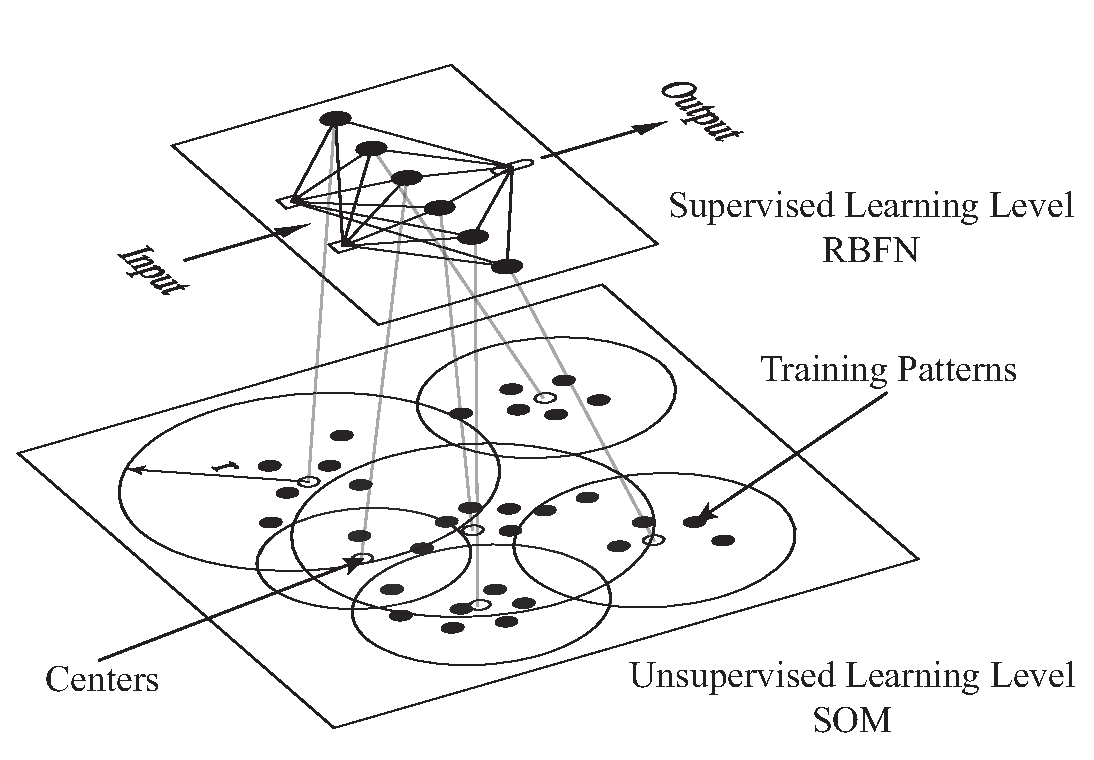
\includegraphics[scale=0.6]{rbf-som.eps}
%    \caption{The two phases of an \RBF\ network training based on \SOMs:
%            (a) self-organized positioning of the \RBF\ centers (unsupervised 
%            learning) and (b) computation of the synaptic weights (supervised
%            learning.}
%    \label{f:rbfn-som}
%\end{figure}


The so-called \textit{Importance Factors} ($IFs$), as proposed by Giotis et al. \cite{LTT_2_018}, can improve the prediction ability of the $RBF$ network. Incorporating $N$ extra coefficients ($I_n, n\!=\!1,N$), the importance of each design parameter on the network response is quantified and exploited in order to increase the overall $RBF$ network prediction quality. High $I_n$ values indicate high sensitivity of the objective function in the vicinity of the design point under consideration with respect to the $n$-th input variable. The $IFs$ are computed by the $RBF$ network as a by-product of the training process and are used to improve the quality of networks' output. 
In detail, each time an improved solution is computed by the $EA$ (index $b$, which stands for the current best), a local $RBF$ network is built and $N$ partial derivatives $\partial o^{(b)} / \partial x_{n}$ are computed using the closed-form response expressions; by doing so, $\partial o^{(b)} / \partial x_{n}$ become the exact derivatives of an approximate function. 
Based on these derivatives, a weighted norm is introduced and used instead of the standard one (i.e.\ instead of eq. \ref{response}), as follows
%
\begin{equation}\label{e:IFcomp}
    \left\|\vec x^{(t)}-\vec c^{(k)}\right\|_{wei} =
    \sqrt{  \sum_{n=1}^N I_n\left(x_n^{(t)}-c_n^{(k)}\right)^2  }
	\mbox{,~where~~~~}
    I_n = { {\left|  {\partial o^{(b)}} \over {\partial x_n} \right|} 
          \over 
  { \sum_{i=1}^{N} \left| {\partial o^{(b)}} \over {\partial x_i} \right| } }
\end{equation}


\subsubsection{Inexact Pre--Evaluation Algorithm}


The algorithm starts as a conventional $(\mu, \lambda)EA$ (by exclusively making use of the exact evaluation model) for the few starting generations until a user--defined minimum number of previously evaluated individuals enter the $DB$. 
Then, the $IPE$ phase starts and, in subsequent generations, instead of evaluating the offspring population on the costly problem-specific model, the following actions are taken:
\newcommand{\apprx}[1]{\tilde{#1}}
\begin{itemize}
\item[]{\bf Inexact Evaluation:}
For each offspring, $\vec{x}\!\in\!P_{\lambda,g}$, the objective function values $\apprx{\vec{F}}(\vec{x})$, are approximated using a local metamodel trained on a small number of data selected from the $DB$. 
%
\item[]{\bf Screening:}
%>>>>
Based on the $\apprx{\vec{F}}(\vec{x})$ values, a provisional
$\Phi$ value (denoted by $\apprx{\Phi}$) is assigned to each
offspring.
%>>>>
\item[]{\bf Exact Evaluation:}
%>>>>
For all $\vec{x}\!\in\!P_{e}$, the ``exact'' objective function values $\vec{F}(\vec{x})$ are computed and stored in the $DB$. 
Practically, this step determines the $CPU$ cost of each generation.
%...................
\end{itemize}


\subsection{Hierarchical Evolutionary Algorithms}

As mentioned in section \ref{EAintro}, an additional way to reduce the optimization turn-around time is by using the so-called hierarchical EA (HEA). HEAs are based on a hierarchical search structure, which consists of a number of semi–autonomously ``evolving'' levels (multi-level structure). Within each level, different evaluation tools, search techniques and/or problem parameterizations can be used, \cite{Herr1999, kn:Sef2000, Desid2003, LTT_2_031, LTT_3_092, LTT_2_036, LTT_2_044, LTT_2_048, LTT_4_05}. Each level solves a different variant of the same problem. Furthermore, adjacent levels may exchange their best individuals according to one- or two-way inter-level communication schemes. The following three hierarchical schemes/modes, schematically presented in fig.\ \ref{allheas}, can also be combined in a single scheme.


\begin{figure}[h!]
    \centering
    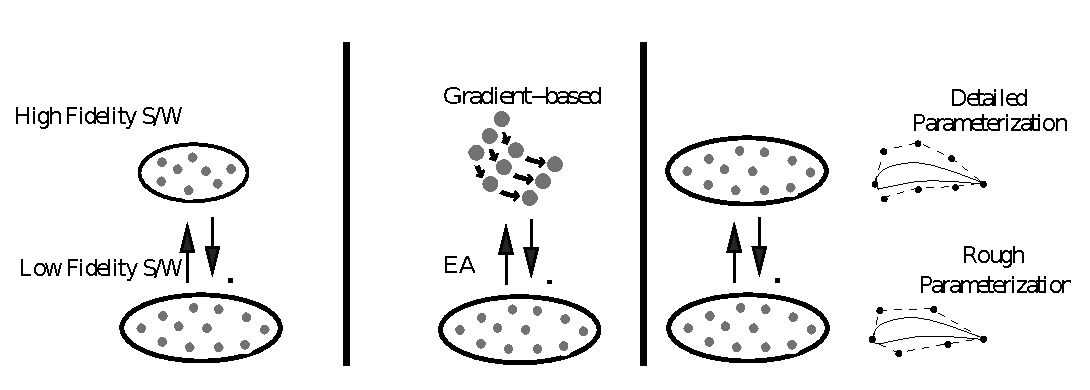
\includegraphics[scale=0.8]{multimodes.eps}
% ------------------------------------------------
    $\mbox{Hierarchical Evaluation~~~~~Hierarchical Search~~~~~~Hierarchical Parameterization}$
%   $\mbox{Hierarchical}~~~~~~~~~~~~~~~~
%    \mbox{Hierarchical}~~~~~~~~~~~~~~~~~~~~
%    \mbox{Hierarchical}$
%   \\
%   $~~~\mbox{ Evaluation }~~~~~~~~~~~~~~~~~~
%    \mbox{   Search   }~~~~~~~~~~~~~~~~~~~
%    \mbox{Parameterization}$
% ------------------------------------------------
    \caption{$HEAs$. Schematic representation of  three
            hierarchical schemes. Left: Hierarchical Evaluation. Middle: Hierarchical Search. Right: Hierarchical Parametrization. All this types can be combined or used separately, at will, utilizing two or more levels.}
    \label{allheas}
\end{figure}      

The three hierarchical schemes are described below:
\paragraph{(a) Hierarchical Evaluation Scheme:}  
The hierarchical evaluation scheme allows the exploitation of a number of different evaluation tools/softwares with different fidelity and cost (computational and/or economical). Each tool is assigned to a different EA or MAEA level. By convention, the lower level undertakes the exploration of the design space by utilizing the low-cost and reduced fidelity tool so as to locate near–optimal solutions at low CPU cost and, then, delivering them to the higher level(s) for further refinement. On the higher level(s), being exploitation-oriented and responsible for delivering optimal solution(s), evaluation tools of higher fidelity and CPU cost are employed. Two–way inter–level communication can be used. So, apart from the migration of promising individuals upwards for them to undergo refinement, higher level individuals may also move downwards so as to stimulate a more exhaustive search in their neighborhood, based on a low-cost evaluation tool. In the hierarchical evaluation scheme, as many DBs as the number of evaluation tools should be maintained. In a two–level algorithm, for instance, the high-fidelity DB, recording entries from evaluations based on the high-level problem–specific tool, is linked to the high level and the associated IPE phase. Next to it, a low-fidelity DB will does the same on the low level. Without loss in generality, differently configured MAEAs can be used on each level. An example of hierarchical evaluation used to handle an industrial application, is presented in fig.\ \ref{HMAEA}, where the higher level is assosiated with a Navier-Stokes equations' solver and the lower level with an Euler one.


\begin{figure}[h!]
\begin{minipage}[b]{1.0\linewidth}
 \centering
 \resizebox*{14cm}{!}{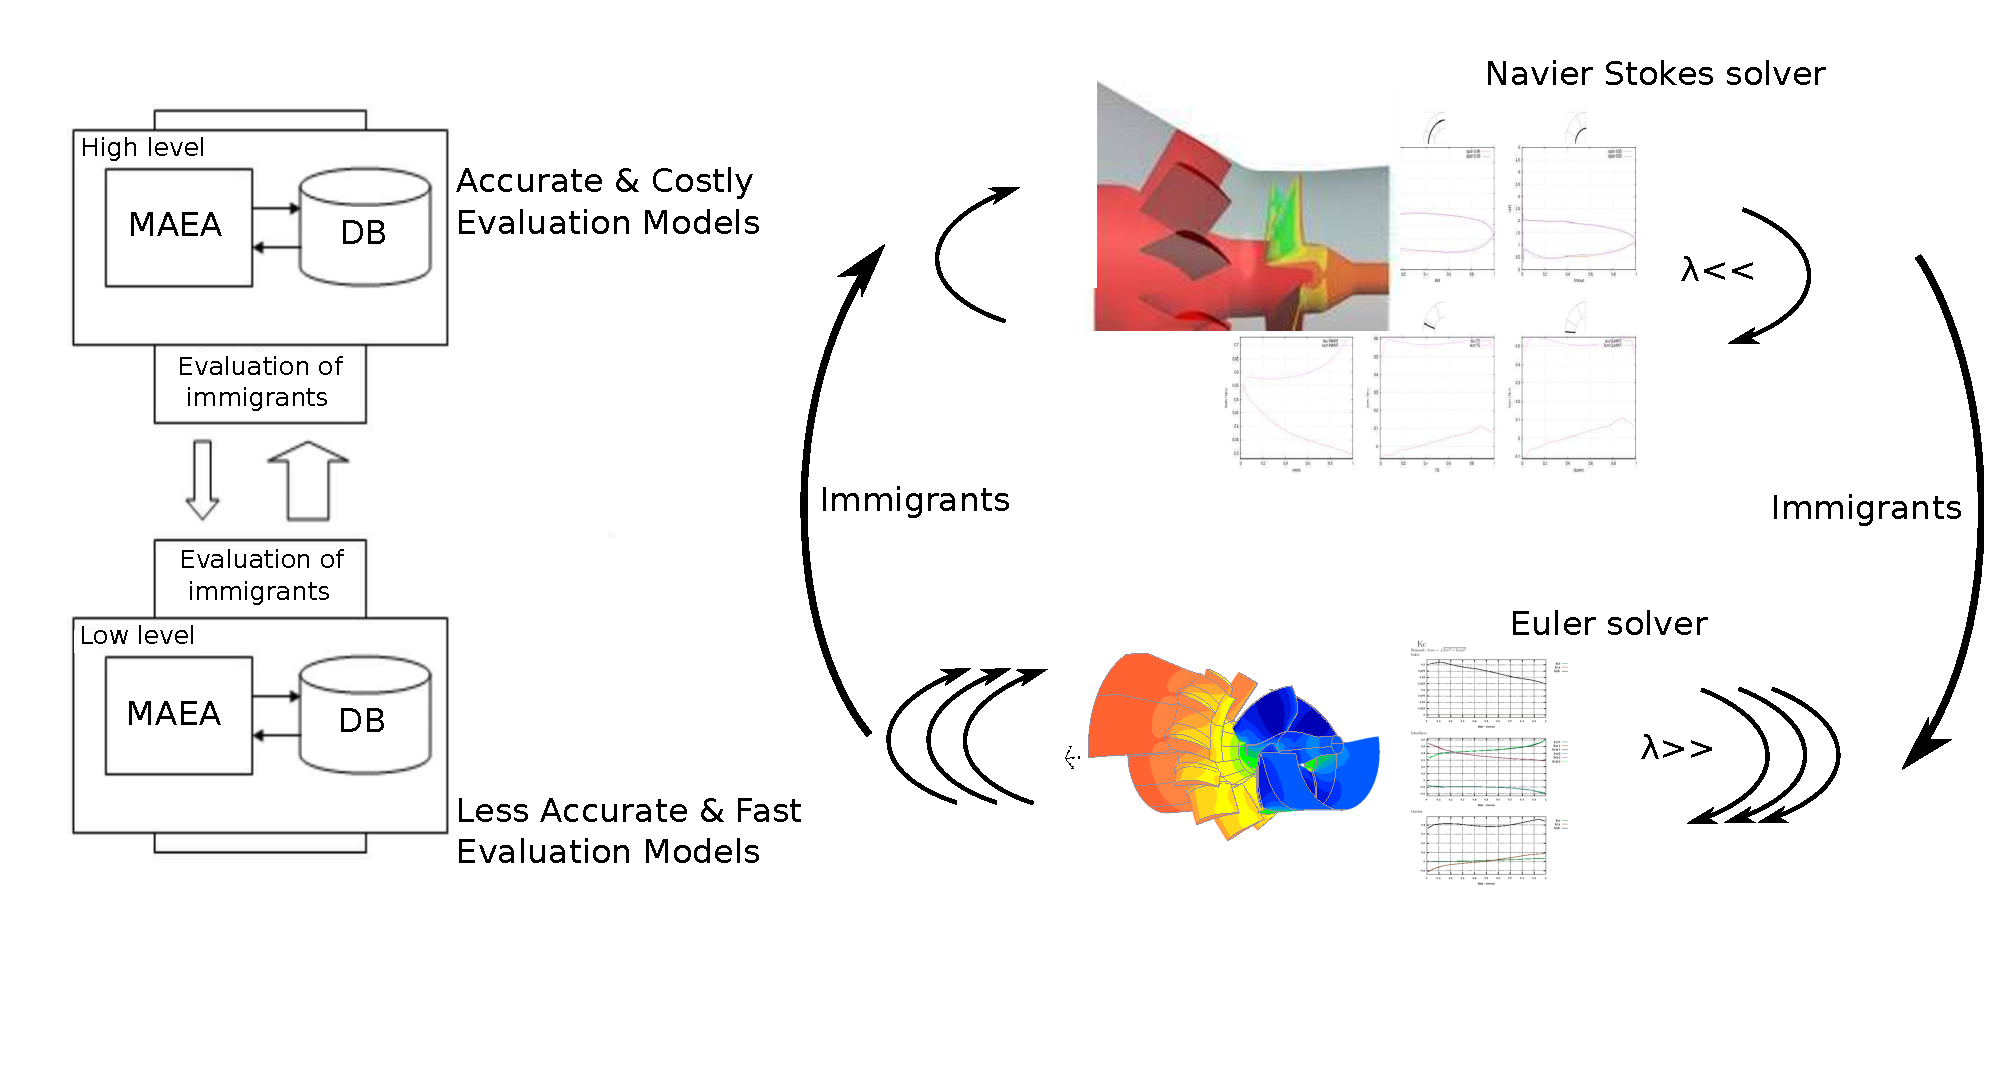
\includegraphics{handmade.eps}}
\end{minipage}
\caption{Left: Schematic representation of a two-level HMAEA (Hierarchical MAEA). The high level is associated with the expensive and accurate model and the lower level with the cheap and, thus, less-accurate one. Communication between the two level is possible in both directions including re-evaluation with the evaluation tool associated with receiving level. Right: Example of a HMAEA used in hydraulic turbine design \cite{LTT_3_094}.}
\label{HMAEA}
\end{figure} 

\paragraph{(b) Hierarchical Search Scheme:}
In hierarchical search scheme, each level utilizes a different search technique and thus becomes able to combine the advantages of EAs with other search methods. In case the objective function gradient can be computed, the combination of EAs with gradient–based methods (GBM) is of great interest. Stochastic methods, such as EAs (DEAs, DMAEAs, etc.), are typically used for the exploration of the design space, on the lower level, exploiting their ability to escape local optima. Then, promising solutions migrate from the low level to its immediate higher one which uses a GBM to efficiently, with minimum turn-around time, locate the nearest optimum. The migration of promising solutions can be bi-directional, to accentuate the exploration capabilities of low-level EAs. The opposite configuration (GBM on the low and EA on the high level) is also possible. Hierarchical search requires particular attention if a GBM is employed to solve MOO problems, by seeking the front of non–dominated solutions. A common practice is to act on a fitness function formed by concatenating weighted objectives, which is appropriate only for convex fronts. Alternatively, as proposed in \cite{LTT_2_036}, the GBM can optimize the same scalar cost function ($\Phi$) used by the EA, computed for instance via the SPEA2 technique, after appropriately approximating its non-differentiable functions. Should a GBM undergo the refinement on any level, methods for computing the gradient of the objective function must be available. In aerodynamic optimization, the computation of the gradient can be based on the adjoint method, \cite{LTT_2_032}, at extra cost which is approximately equal to that of solving the flow equations.


\paragraph{(c) Hierarchical Parameterization Scheme:}
In hierarchical parameterization different parameterizations are  associated with each level. Typically a rough parameterization with a reduced number of design variables is associated with the lower level, where rough designs are quickly detected due to the small dimensionality of the problem. On the other hand, a detailed parameterization is associated with the higher level.  The hierarchical or multi-level parameterization scheme should be configured in a way that makes all but the high level not affected (or, at least, slightly affected) by the curse of dimensionality. During the inter-level migration steps, a few promising solutions detected on the low level(s) are sent to the higher level(s) for refinement. This hierarchical scheme is suitable for shape optimization problems in which the design vector comprises the coordinates of control points of parametric curves and surfaces since, increasing or decreasing the number of control points via knot insertion and removal algorithms, allows exact (upwards) or approximate (downwards) transformations of the design vectors.


% ---------------------------------------------------------------------------
% ----------------------- end of thesis sub-document ------------------------
% ---------------------------------------------------------------------------
					% EAs
% this file is called up by thesis.tex
% content in this file will be fed into the main document
\chapter{Knowledge-Based Design} % top level followed by section, subsection
%: ----------------------- paths to graphics ------------------------

% change according to folder and file names
\ifpdf
    \graphicspath{{3/figures/PNG/}{3ures/PDF/}{2.5/figures/}}
\else
    \graphicspath{{3/figures/EPS/}{3/figures/}}
\fi

%: ----------------------- contents from here

%\begin{flushright}
%An amazing thing, the human brain
%\linebreak
%apable of understanding incredibly complex
%\linebreak
%and intricate concepts. Yet at times unable
%\linebreak
%to recognize the obvious and simple.
%\linebreak
%Jay Abraham 
%\end{flushright}

\label{KBDchapter}
It is common for all companies to keep archives of previous successful designs. As a consequence, irrespective of the design method adopted, there are often reasons for new designs to be based on ``similar" previous ones, instead of starting the design procedure from scratch. As a matter of example, if for instance a new turbomachinery rotor is to be designed, a useful ``similar'' design might be a rotor successfully  designed in the past for ``slightly'' different operating conditions and/or ``slightly'' different objectives or constraints. 
In some cases, these designs might have been performed enough time ago, using ``old-fashioned'' design procedures according to different paremeterizations. In general, the term Knowledge-Based System (KBS) \cite{Akerkar:2009:KS:1795845} is used to describe methods and processes for designing new products, engines, services etc.\ based on stored/archived knowledge which is available in the form of previous successful designs.                

In this thesis, a new design method, to be referred to as  Knowledge-Based Design (KBD), which combines EAs with principles and concepts from Knowledge-Based Systems (KBS) in order to create an automated design procedure, is proposed. It employs a KBS similar to Case-Based Reasoning (CBR) \cite{kolodner_1991,kolodner_1993,slade_1991,riesbeck_1989}, in order to utilise/exploit the availability of an archive of successful designs. In the design of aero- or hydrodynamic shapes, a pattern of similar geometries often occurs when dealing with similar problems. For example, the optimal airfoil, regarding objective(s) ``A" and constraint(s) ``B", of a compressor cascade operating at conditions ``C" and inlet flow angle $\alpha_1$ (where ``C'' includes everything but $\alpha_1$) will be, more or less, similar to the airfoil of a different compressor designed for the same ``A", ``B" and ``C" and inlet flow angle equal to $\alpha_1\!+\!1^o$.  Therefore, if a design is optimal for a set of different/neighbouring conditions, it still holds valuable information about the design space that can be exploited in order to speed-up the design process. This is the main purpose of the proposed KBD method which shares the advantages of both EAs and KBS.    

In more detail, from the CBR point of view, the proposed methodology achieves in creating a fully automated and time-efficient \textit{revise} step, this is the step that adapts the existing ``similar" designs so as to make them perform optimally at the new operating conditions and/or according to the new objectives. In this thesis, this is achieved by using an EA as a revise tool. In order to have a cost-efficient procedure, capable for being routinely used in an industrial environment, additional EA speed-up techniques, mainly the use of metamodels (MAEA, section \ref{MAEApar}), are employed. The straightforward way to achieve this goal would be to simply inject the ``similar" archived designs into the initial population of an EA, by replacing some of the randomly generated population members.
In contrast, the method proposed in this thesis utilizes statistical analysis to introduce a new set of design variables, based on the archived designs, in order to further speed-up the EA itself. This is achieved through:  
%Regarding EAs the proposed method achieves three important goals: 
\begin{description}
  \item[a)]The significant reduction in problem dimension (i.e.\ the number of design variables handled by the EA), thus improving both the EA (faster convergence to the optimal solution) and MAEA efficiencies (use of ANNs as metamodels  with greater prediction accuracy and without delaying the start of the IPE phase, as described in section \ref{MAEApar}). 
  \item[b)]The automatic definition of the newly introduced design variables' (to be referred to as optimization variables, to distinguish them from the design variables used to parameterize the geometry) range; the designer overcomes the burden of arbitrarily guessing their lower and upper bounds and, therefore, eliminates the possibility of accidentally excluding search sub-areas corresponding to the optimal design. 
    \item[c)]The association of degrees of importance to the optimization space regions. Practically, higher probability to host candidate solutions is given to the regions of the design space pinpointed by the statistical analysis of the archived ``similar" designs, based on a pre-defined probability distribution. This allows the exploration of extended design spaces, with different levels of importance associated with different sub-regions, according to statistics.
\end{description}

%All the above allow the exploitation of extended design spaces, both in number of design variables and effective range for each one of them, in an efficient way by exploiting the information incorporated in archived "similar" designs.     

\section{Knowledge-Based Systems (KBS)}  
KBS \cite{Akerkar:2009:KS:1795845}  are systems based on methods and techniques of artificial intelligence. Their core components are the knowledge base and inference mechanisms. In this thesis, a KBS named Case-Based Reasoning (CBR) \cite{kolodner_1991} is combined with EAs, in an optimal way, giving rise to the KBD method. For reasons of clarity, a brief introduction to the CBR method follows, before presenting the proposed KBD method.  

%***********************************************************************
\subsection{Case-Based Reasoning Method - Principles}
%***********************************************************************
CBR, \cite{kolodner_1991,kolodner_1993,slade_1991,riesbeck_1989}, can be seen as a problem solving method that reuses past cases and experience to conceive a solution to the current problem, 
whereas other major artificial intelligence techniques rely on mapping generalized 
relationships between problem descriptions and conclusions. CBR has the advantage 
of utilizing  experience based on past successful problem solutions. 
The main tasks of a CBR system is to identify the problem in hand, find one or 
more similar past case(s), use this information to suggest a solution to the current 
problem and update the system by learning from this experience.      

\label{History} The origins of CBR dates back to the work by
Schank and Abelson in 1977, \cite{Schank_Abelson_1977}. They proposed that general 
human knowledge about situations is recorded as scripts that allow extracting 
 expectations and inferences. Scripts were proposed as structures for conceptual 
memory describing information about stereotypical events. However, experiments 
showed that this is not a complete theory of memory representation since people 
often confuse events with similar scripts. These conform with 
concept formulation, problem solving and experimental learning theories within 
philosophy and psychology, \cite{tulving_1977,smith_1978}. 

Schank continued to investigate the role of previous situations (i.e.\ cases) 
and situation patterns in both problem solving and learning, \cite{Schank_1982}.  
Simultaneously, Gentner, \cite{genter_1983}, developed a  
theoretical framework for analogy also relevant to CBR. Significant references to CBR can also be found in 
Wittgensteins observation, \cite{wittgestein_1953}, that natural concepts are in fact 
polymorphic and cannot be classified by a single set of necessary and sufficient 
features; instead they can be defined by a set of instances (i.e.\ cases) with family 
resemblances. The latter work has been cited as the philosophical basis for CBR by Aamondt and Plaza, \cite{aamond_plaza_1994}.

Though the roots of CBR could be claimed by several scientists, it was Schank and his co-workers who, in the early 80's, developed a cognitive model which the first CBR applications were based upon. Kolonder developed the first CBR system named CYRUS, \cite{kolodner_1983a,kolodner_1983b}, which was an implementation of Schank's dynamic memory model. Later, its case-memory model served as the basis for several other CBR systems and was used in various disciplines ranging from law, \cite{ashley_1988,rissland_skalak_1989}, to civil engineering, \cite{whatson_abdullah_1994,moore_1994}.

\label {CBR}  The classical definition of CBR was coined by Riesbeck and Schank, \cite{riesbeck_1989}: \textit{``A case-based reasoner solves problems by using or adapting solutions to old problems"}. This clearly defines what a CBR system can do, without however determining the way of doing it. This can be graphically understood by the so-called CBR-cycle (fig.\ \ref{cbr}).  The CBR-cycle is based on four logical steps, as defined by Aamodt and Plaza, \cite{aamond_plaza_1994}, which are often referred to as the four REs: 

\begin{itemize}
  \item RETRIEVE the most ``similar" case(s),
  \item REUSE the retrieved case(s) for the problem in hand,
  \item REVISE the case(s), if necessary, and
  \item RETAIN the new solution in the archive for future use.
\end{itemize}
The four REs can be represented by a schematic cycle, fig.\ \ref{cbr}.

In the proposed KBD method, the REVISE step is undertaken by an EA which automatically combines the RETRIEVED cases without requiring human intervention. Recall that the traditional CBR method requires a human expert to undertake task.  

%\figuremacroW{cbr}{Schematic cycle representing the CBR-cycle}{0.5}
\begin{figure}[h!]
\begin{minipage}[b]{1\linewidth}
 \centering
 \resizebox*{!}{10 cm}{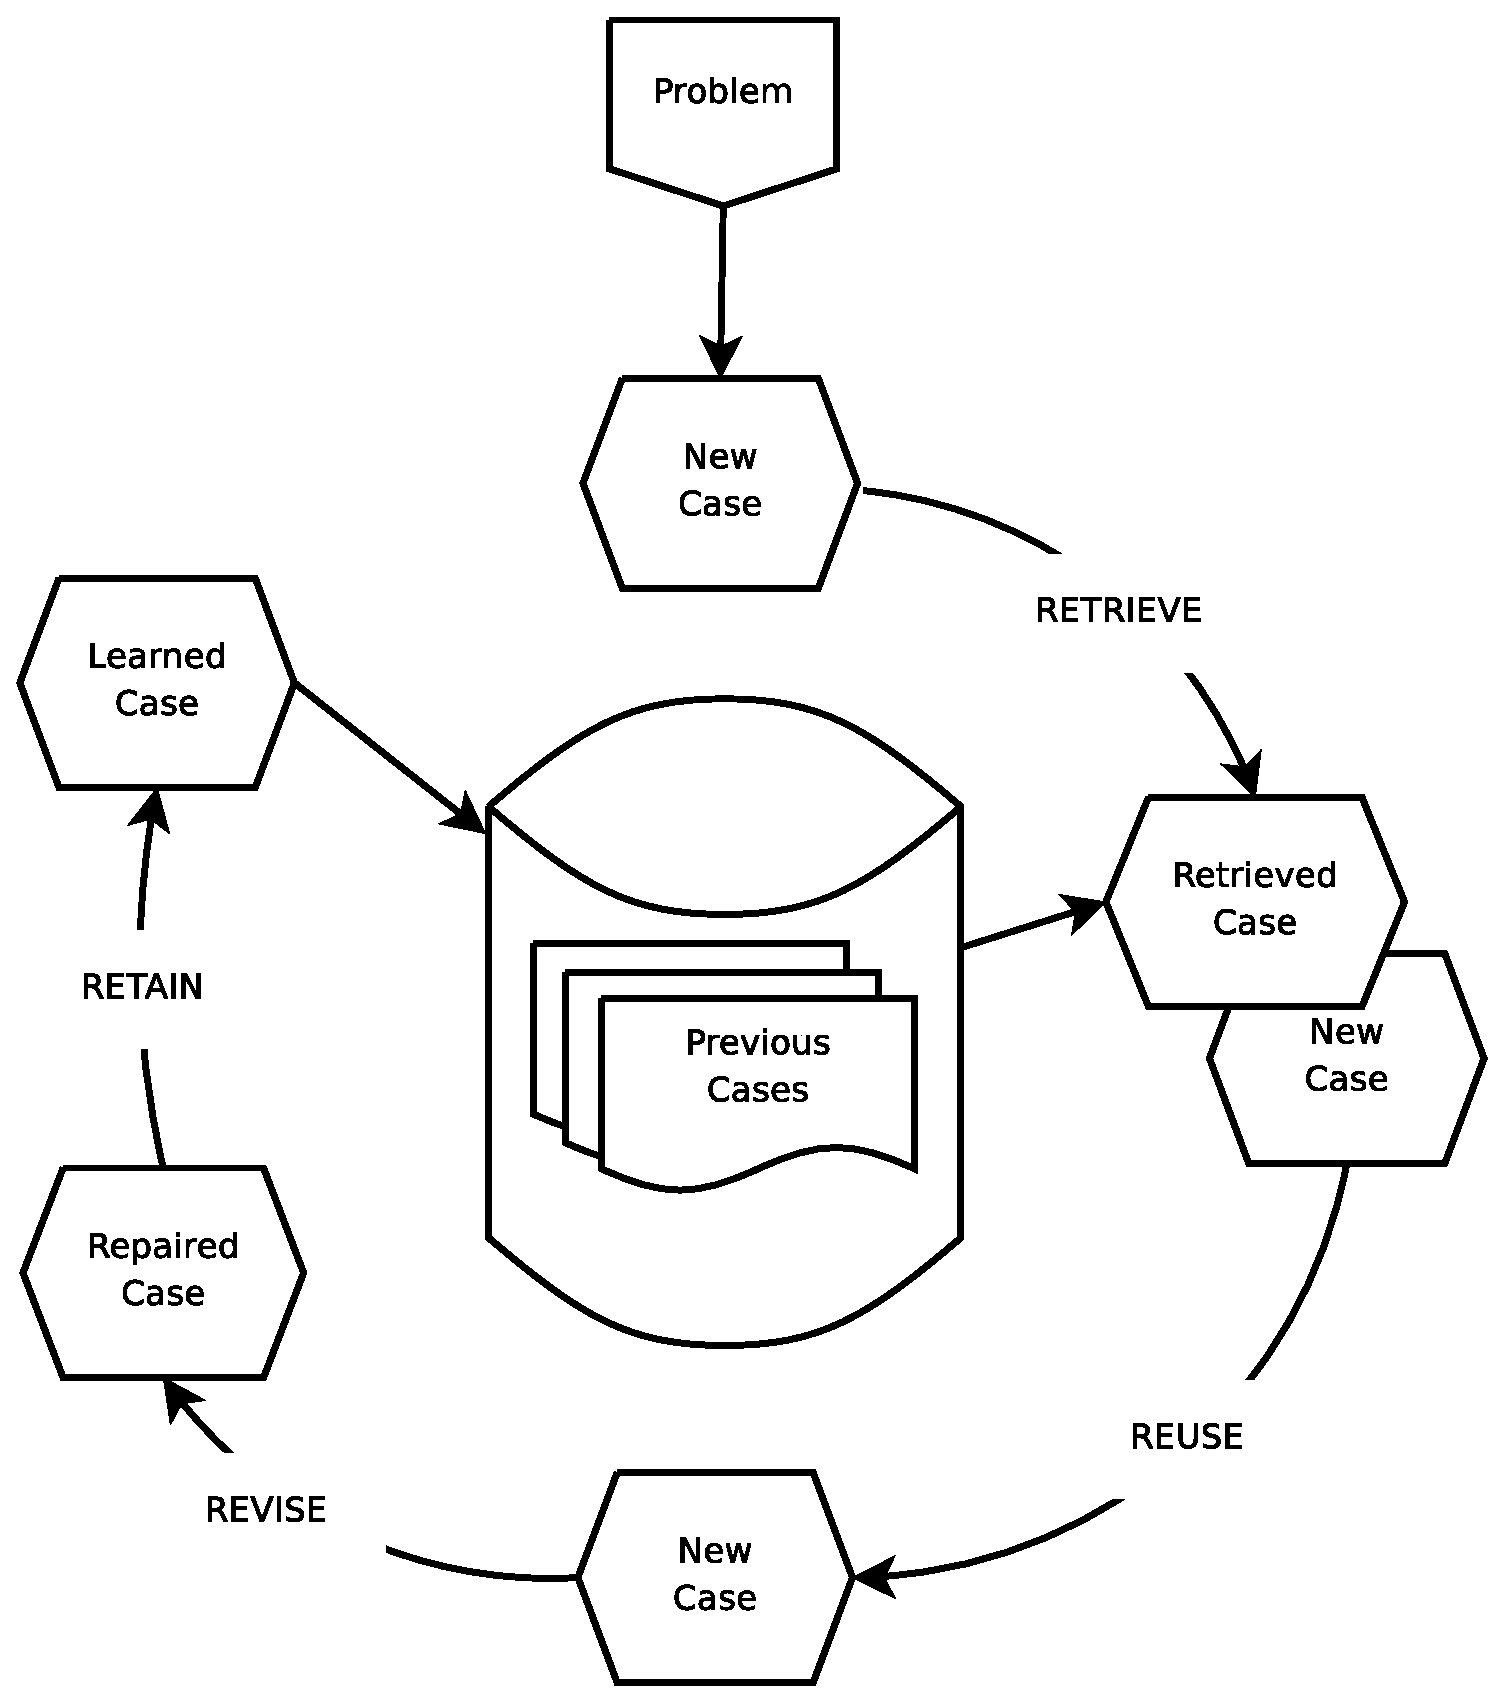
\includegraphics{cbr.eps}}
\end{minipage}
\caption{Schematic representation of the CBR-cycle; from \cite{aamond_plaza_1994}.} 
\label{cbr}
\end{figure}

%%%%%%%%%%%%%%%%%%%%%%%%%%%%%%%%%%%%%%%%%%%%%%%%%%%%%%%%%%%%%%%%%%%%%%%

\section{The KBD Method}

%In case of shape design problems in fluid mechanics with specific characteristics in a specific environment, due to the nature of the problem, the solution is always complex. Thus the need of adaptation (revise) is almost certain. \textit{Null adaptation is useful for problems involving complex reasoning but with a simple solution.}

In order to have a fully automated REVISE step, a set of adaptation rules must replace human intervention. These rules take into account the deviations of the proposed solution from the desired one and suggest an improved proposal. The rules governing the evolution of species ideally fit the above description. So, in this thesis, an EA is proposed to undertake the REVISE step. 

Therefore, the present method aims at extending the optimization method by making it capable to accommodate and exploit pieces of useful information archived during previous relevant successful designs. The KBD method is much more elaborated than the simple and straightforward injection of retrieved designs in the initial population of an EA, where they replace some of the randomly generated ones. Instead, the KBD method  introduces a new set of unknowns, the so-called optimization variables, to be used by the EA, instead of the design variables. In case of complex 3D geometries, such as those involved in the field of thermal and hydraulic turbomachines, the number of design variables is much greater and this slows the design-optimization process down. The optimization variables are introduced by expressing the candidate solutions as points in the optimization space, which is the space defined by the design vectors of the retrieved geometries as vector bases. The role of the optimization algorithm is to find the value set (or sets, for more than one objectives, in problems where the Pareto front of non-dominated solutions is sought) of the optimization variables which yields optimal performance. Since the number of optimization variables is much less than the number of design variables, the number of degrees of freedom is reduced and the EA or MAEA CPU cost is expected to be much lower.

\subsection{Optimization Variables's Definition}
In this section, the optimization variables introduced by the proposed KBD method are presented. Assume that a small number (m) of previous designs are retrieved from the archive. These designs must correspond to similar problems, as already discussed. For the proposed method, it is necessary  for the retrieved geometries to be expressed in terms of the same parameterization. If techniques able to transform a parameterization scheme to any other (within a degree of accuracy, of course) are available, this task is straightforward. Let us denote by $GEO_i=(x_1^i,x_2^i,....,x_N^i)$, $i\!=\!1,m$ the m archived designs, with $N$ design variables each.

The set of optimization variables can be defined, without yet associating any degree of importance to the optimization space subregions, by assuming that each new design $x_j^{new}$ results from the combination of the $m$ archived designs, weighted by the  $w_i$ $(i=1,m)$, or

\begin{eqnarray}
   x_j^{new} = \frac{\sum_{i=1}^{m}w_i x_j^i}{\sum_{i=1}^{m}w_i },~~~ j=1,...,N 
   \label{linear} 
\end{eqnarray}
Without loss in generality, one may assume that $w_i \in [0,1]$. 

Next step is the association of degrees of importance to the optimization space regions. This is achieved by rewriting eq. \ref{linear} as

\begin{eqnarray}
   x_j^{new} = \Phi _j^{-1} (\frac{\sum_{i=1}^{m}w_i \Phi _j(x_j^i)}{\sum_{i=1}^{m}w_i }) 
   \label{non-linear} 
\end{eqnarray}
through the introduction of the sigmoid cumulative distribution function $\Phi$,  \cite{Kiemele}, according to a user-defined probability distribution function. If the normal distribution function is used, $\Phi$ is given by

\begin{eqnarray}
   \Phi _{\mu \sigma ^2} (x)= \frac{1}{\sigma\sqrt[2]{2\pi}}\int _{-\infty}^x exp(\frac{-(u-\mu)^2}{2 \sigma^2}) 
   \label{cdf} 
\end{eqnarray}
where $\mu$ is the mean value and $\sigma$ the standard deviation of each design variable (j). Schematically,
\begin{eqnarray}
		\left( {\begin{array}{c}
 		x_1^1  \\
 		\vdots  \\
 		x_N^1	\\
 		\end{array} } \right) 
 		\left( {\begin{array}{c}
 		x_1^i  \\
 		\vdots  \\
 		x_N^i	\\
 		\end{array} } \right)
 		\left( {\begin{array}{c}
 		x_1^m  \\
 		\vdots  \\
 		x_N^m	\\
 		\end{array} } \right) \rightarrow
		\left( {\begin{array}{c}
 		\mu _1  \\
 		\vdots  \\
 		\mu _N  \\
 		\end{array} } \right)
		\left( {\begin{array}{c}
 		\sigma _1  \\
 		\vdots  \\
 		\sigma _N  \\
 		\end{array} } \right)
   \label{cdf-matrix} 
\end{eqnarray}


 
%Among other, the set of the archived solutions reveals the statistical distribution of each design variable and, consequently, this can be used both to introduce importance to the design space regions and also set the bounds of the design space. This is achieved by, instead of eq. \ref{linear}, the nonlinear equations

%
%are to be used in order to define the new optimization variables. In eq. \ref{non-linear}, $\Phi _j$ are appropriate nonlinear functions. Based on the assumption that the retrieved designs correspond to operating conditions correlated to the new ones, the new design should conform to a normal distribution. Should this be the case, the sigmoid cumulative distribution function could be used for $\Phi _j$  \cite{Kiemele}. 

Since the m retrieved designs are usually located ``around'' the desired one in the operating conditions space and based on the assumption that this information is, more or less, transferable to the design space, the  normal probability distribution is used to assign degrees of importance throughout this thesis. In a simplified example, the above statement says that: Assume that airfoil A with design variables vector $\vec{x}_A$ is optimal, regarding objective(s) ``O'', when operating at conditions ``C''. Assume, also, that at these conditions the flow turning is equal to $\Delta a\!=\!40^o$. Also,  that design B, or $\vec{x}_B$,  is optimal regarding the same objectives at the same conditions and delivers flow turning equal to $\Delta a \!=\!41^o$. Considering the same objectives ``O'' and the same conditions ``C'', if the optimal airfoil which delivers flow turning equal to $\Delta a\!=\!40.5^o$ is sought, the optimal design N, or $\vec{x}_N$, would, most probably, be close to  $\frac{\vec{x}_A+\vec{x}_B}{2}$ which is the vector of the mean values of the design variables of the retrieved geometries A and B. It is reminded that, if the normal probability distribution is used for importance assignment, the regions near the mean value of each design variables will be assigned the highest importance and, therefore, highest probability to accommodate candidate solutions. In case the user knows in advance that, for this particular problem, the above statement is not true, he might exchange the normal distribution with the appropriate probability distribution of his choice.           

The use of the cumulative distribution function of the normal probability distribution, eq.\ \ref{cdf}, practically assumes the bounds of $b_i$ to be within $\mu _i \pm 3\sigma _i$, \cite{Kiemele}. To overcome this limitation, a single extrapolation variable $\Psi$ which multiplies all $\sigma$ values computed based on the archived designs and extends the search space outside $\mu _i \pm 3\sigma _i$, is optionally introduced. $\Psi$ is multiplied with the computed standard deviations to yield the ones used in eq.\ \ref{cdf}, as follows


\begin{eqnarray}
		\left( {\begin{array}{c}
 		\sigma _1  \\
 		\vdots  \\
 		\sigma _n  \\
 		\end{array} } \right) =
 		\Psi  
 		\left( {\begin{array}{c}
 		\sigma _1^{computed}  \\
 		\vdots  \\
 		\sigma _n^{computed}  \\
 		\end{array} } \right)
   \label{cdf-matrix} 
\end{eqnarray}


If the available archived designs are not that many, which often is the case, then $m$ is a significantly small integer.  With either eq.\ \ref{linear} or \ref{non-linear}, an optimization problem with only $m$ weights as unknowns may loose its flexibility. Such a method may overcome the curse of dimensionality (since the number of optimization variables is  noticeably lower than $N$) but may lead to sub-optimal solutions. To overcome this, the grouping of those design variables which are ``co-related''. Relevant design variables such as, for instance, those defining the mean camber surface angle at the leading edge etc.\ are grouped together. After forming these groups, a different weight is associated with each one of them. The new weights are denoted by $w_{i,k}$, where the first index corresponds to the $i^{th}$ design basis and the second one to the $k^{th}$ group of design variables (where $b_i$ belongs to). Finally, instead of either eq.\ \ref{linear} or \ref{non-linear}, the expression


\begin{eqnarray}
   x_j^{new} = \Phi _j^{-1} (\frac{\sum_{i=1}^{m}w_{i,k} \Phi _j(x_j^i)}{\sum_{i=1}^{m}w_{i,k} }),~ k=f(j) 
   \label{non-linear2} 
\end{eqnarray}
can be used. 

Based on eq.\ \ref{non-linear2}, an optimization problem with $m  K$ unknowns (or $m K\!+\!1$, to also account for $\Psi$), where $K$ is the number of design variable groups, is formulated. Population-based search methods, such as EAs (or MAEAs), with the proposed parameterization, may locate the global optimum much more efficiently than an EA (or MAEA) based on the conventional parameterization. This is demonstrated on the solution of  thermal (section \ref{Drela1}) and hydraulic (section \ref{Francis-runners}) turbomachinery design-optimization problems. 


%\begin{figure}[h!]
%\begin{minipage}[b]{0.9\linewidth}
% \centering
% \resizebox*{9cm}{!}{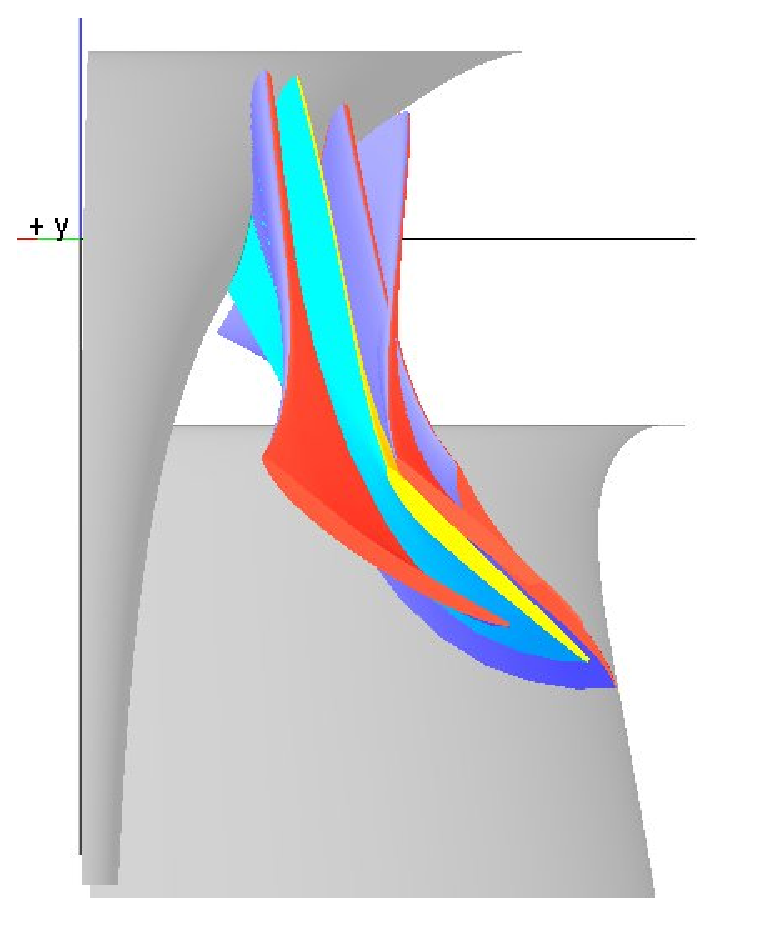
\includegraphics{cbr_r.eps}}
%\end{minipage}
%\caption{A new Francis blade (section \ref{Francis-runner}) (\ifcolore light blue and yellow\else light gray\fi) is designed on the basis of 3 %archived designs (\ifcolore dark blue and red\else dark gray\fi).} 
%\label{CBRtemp1}
%\end{figure}


%\begin{figure}[h!]
%\begin{minipage}[b]{0.9\linewidth}
% \centering
% \resizebox*{12cm}{!}{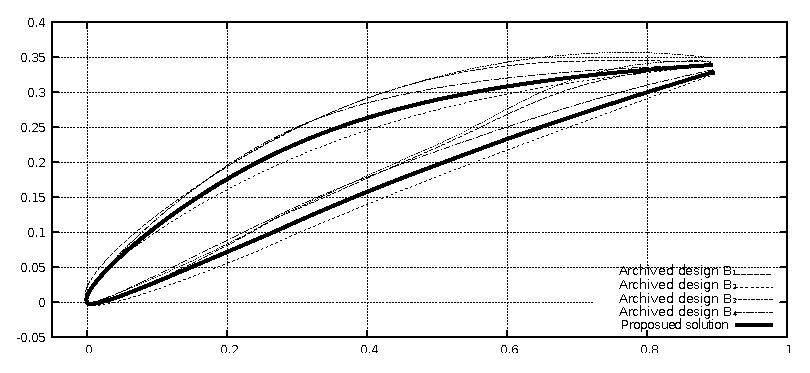
\includegraphics{blade.eps}}
%\end{minipage}
%\caption{A new airfoil (continuous line) is designed on the basisof 4 archived designs (dotted lines).} 
%\label{CBRtemp2}
%\end{figure}

%Two applications of the KBD method, for the design of a Francis hydraulic turbine and a compressor cascade, are presented in fig.\ref{CBRtemp1} and fig.\ref{CBRtemp2} respectively. The Francis blade (fig.\ref{CBRtemp1}) is generated from the KBD method using three archived designs (\ifcolore dark blue designs\else dark gray\fi). Using the KBD method a significant  reduction in the design parameters was achieved, from $336$ to $19$  ($3$ bases $\times 6$ groups $+1$ extrapolation parameter) (for more information see section \ref{Francis-runner}). The compressor cascade (fig.\ref{CBRtemp2}) is design using four archived designs (dotted lines) and the number of design parameters was decreased from 27 to 13 ($4$ bases $\times 3$ groups $+1$ extrapolation parameter).

\section{Design of a Compressor Cascade using KBD}
\label{Drela1}
The design of a 2D compressor cascade operating at $M_1\!=\!0.54$, $a_1\!=\!44^o$ and $Re\!=\!4\times10^5$ (Reynolds number based on the chord) for minimum total pressure losses is sought. Losses are measured in terms of the total pressure loss coefficient 
\begin{eqnarray}
   \omega=\frac{p_{t1}-p_{t2}}{p_{t1}-p_1}
   \label{omegaLosses} 
\end{eqnarray}
where indices $1$ and $2$ denote the cascade inlet and outlet, respectively. 
The blade airfoil is designed subject to a number of aerodynamic and geometrical constraints: the optimal airfoil must turn the flow by more than $30^o$ and its thickness at three chordwise positions ($0.3c$, $0.6c$ and $0.9c$) must be greater than $0.10c$, $0.08c$ and $0.01c$,  respectively.     

The airfoil shape is parameterized based on the mean-camber line shape and thickness distributions (separately for the pressure and  suction sides). All of them are parameterized using NURBS. The mean-camber line parameterization ``introduces'' three degrees of freedom, namely the leading edge (LE) angle, the trailing edge (TE) angle and the weight associated with the second control point. The suction side thickness distribution is controlled by $9$ design variables, namely the $x$ and $y$ coordinates as well as the weights of three, out of the five, internal NURBS control points. The first and last control points are fixed at the predefined LE and TE positions. The pressure side thickness distribution is controlled via 15 design variables, standing for the $x$ and $y$ coordinates as well as the weights of five, out of the eight, internal control points. The first and last control points are fixed at the predefined LE and TE positions and the location of the second point is determined by the requirement of first-order continuity at the LE.  The total number of design variables describing each candidate solution is $27$, fig.\ \ref{CBRparam}. 

\begin{figure}[h!]
\begin{minipage}[b]{1\linewidth}
 \centering
 \resizebox*{15cm}{!}{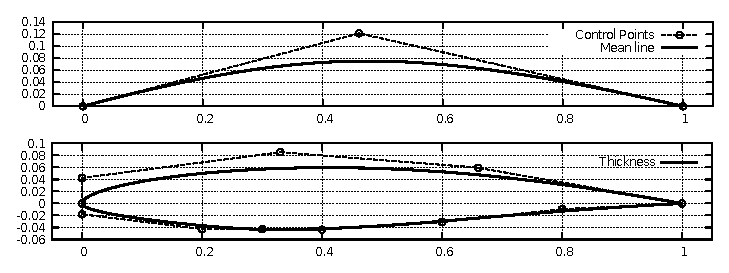
\includegraphics{airf.eps}}
\end{minipage}
\caption{Design of a compressor cascade using KBD: Top: parameterization of the mean-camber line with $3$ control points. Bottom:  parameterization of the thickness distributions with NURBS using $5$ control points for the suction side and $8$ for the pressure side. The total number of design variables is $27$.} 
\label{CBRparam}
\end{figure}

The KBD method will be assessed through the comparison of a traditional MAEA with a KBD-MAEA. For both of them, $\mu=20$, $\lambda=60$ and $\lambda_e=6$. Both cases use local RBF networks as metamodels, which are trained on a small number of training patterns (min.\ 10; max.\ 20 patterns). For the KBD-MAEA, the IPE phase starts after the first $100$ individuals are stored in the DB of previously evaluated individuals. On the other hand, for the MAEA run, $400$ individuals must be stored in the DB before the IPE phase starts. The earlier start of the IPE phase during the KBD-MAEA, as opposed to the MAEA, is due to the reduced number and range of the optimization variables. The KBD-MAEA uses $13$ instead of $27$ design variables  which would be the case if the standard shape parameterization was used. The evaluation software is an integral boundary layer method, \cite{Drel1987}. The maximum number of calls to the evaluation software is $1500$ in all cases, so as to compare them based on the same CPU cost; this is the only termination criterion used.              

Four archived designs were retrieved and used as design space basis vectors in order to define the optimization variables used by the KBD method. 
The archived designs have been designed for operation at different but neighbouring conditions, namely:
%\pagebreak
\begin{itemize}
\item{\textbf{Archived design $B_1$:}} designed for $M_1=0.55$ and $a_1=45^o$, fig.\ \ref{CBR_a}.
\item{\textbf{Archived design $B_2$:}} designed for $M_1=0.50$ and $a_1=40^o$, fig.\ \ref{CBR_b}.
\item{\textbf{Archived design $B_3$:}} designed for $M_1=0.52$ and $a_1=42.5^o$, fig.\ \ref{CBR_c}. 
\item{\textbf{Archived design $B_4$:}} designed for $M_1=0.58$ and $a_1=48^o$, fig.\ \ref{CBR_d}.
\end{itemize}
At their design conditions (see above) the archived geometries perform as follows: 
\begin{itemize}
\item{\textbf{Archived design $B_1$:}} $\omega=0.01976$ and $\Delta a=37.1^o$.
\item{\textbf{Archived design $B_2$:}} $\omega=0.01845$ and $\Delta a=24.4^o$.
\item{\textbf{Archived design $B_3$:}} $\omega=0.02027$ and $\Delta a=36.3^o$.
\item{\textbf{Archived design $B_4$:}} $\omega=0.01877$ and $\Delta a=36.6^o$.
\end{itemize}
The four retrieved airfoils, operating at the new flow conditions ($M_1=0.54$, $a_1=44^o$), without any modification in their shape, perform as follows:
\begin{itemize}
\item{\textbf{Archived design $B_1$:}} $\omega=0.0207$ and $\Delta a=36.3^o$.
\item{\textbf{Archived design $B_2$:}} $\omega=0.0278$ and $\Delta a=27.8^o$.
\item{\textbf{Archived design $B_3$:}} $\omega=0.0201$ and $\Delta a=37.5^o$.
\item{\textbf{Archived design $B_4$:}} $\omega=0.0237$ and $\Delta a=33.1^o$.
\end{itemize}
From the aforementioned $\omega$ and $\Delta a$ values, the necessity for a \textit{REVISE} step becomes obvious since all four retrieved airfoils suffer from relatively high losses and some of them fail to respect the flow turning constraint at the new flow conditions. These four designs were injected in the starting population of the MAEA, either with or without KBD.  

\begin{figure}[h!]
\begin{minipage}[b]{1\linewidth}
 \centering
 \resizebox*{15cm}{!}{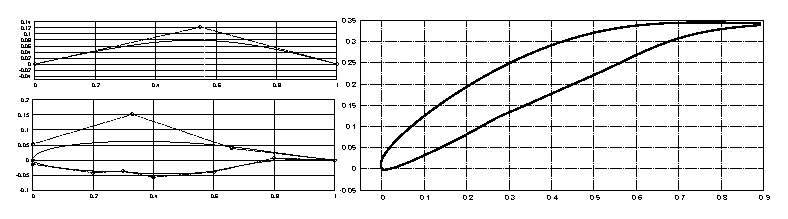
\includegraphics{blade_a.eps}}
\end{minipage}
\caption{Design of a compressor cascade using KBD: Archived design $B_1$.} 
\label{CBR_a}
\end{figure}

\begin{figure}[h!]
\begin{minipage}[b]{1\linewidth}
 \centering
 \resizebox*{15cm}{!}{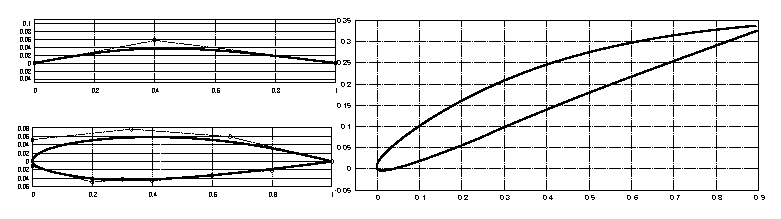
\includegraphics{blade_b.eps}}
\end{minipage}
\caption{Design of a compressor cascade using KBD: Archived design $B_2$.} 
\label{CBR_b}
\end{figure}

\begin{figure}[h!]
\begin{minipage}[b]{1\linewidth}
 \centering
 \resizebox*{15cm}{!}{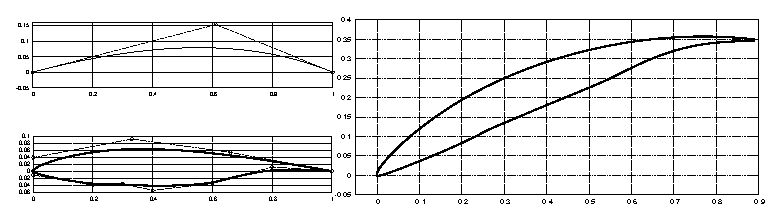
\includegraphics{blade_c.eps}}
\end{minipage}
\caption{Design of a compressor cascade using KBD: Archived design $B_3$.} 
\label{CBR_c}
\end{figure}

\begin{figure}[h!]
\begin{minipage}[b]{1\linewidth}
 \centering
 \resizebox*{15cm}{!}{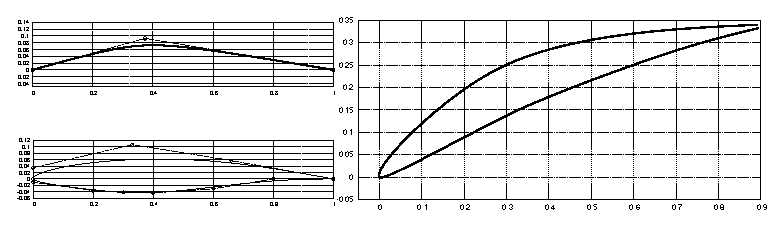
\includegraphics{blade_d.eps}}
\end{minipage}
\caption{Design of a compressor cascade using KBD: Archived design $B_4$.} 
\label{CBR_d}
\end{figure}



\begin{figure}[h!]
\begin{minipage}[b]{1\linewidth}
 \centering
 \resizebox*{15cm}{!}{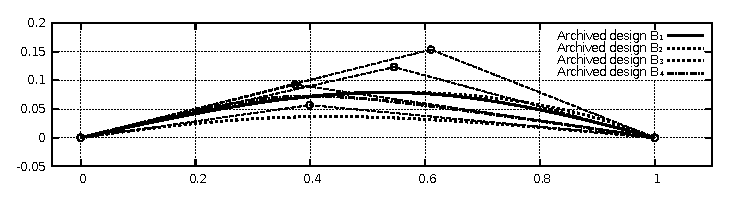
\includegraphics{mean_s.eps}}
\end{minipage}
\caption{Design of a compressor cascade using KBD: Mean-camber lines of the four bases. The observed great variance recommends the use of very extended design variable ranges during the EA-based optimization. This significantly deteriorates EA efficiency and makes the use of metamodels questionable. } 
\label{CBRDmm}
\end{figure}

\begin{figure}[h!]
\begin{minipage}[b]{1\linewidth}
 \centering
 \resizebox*{15cm}{!}{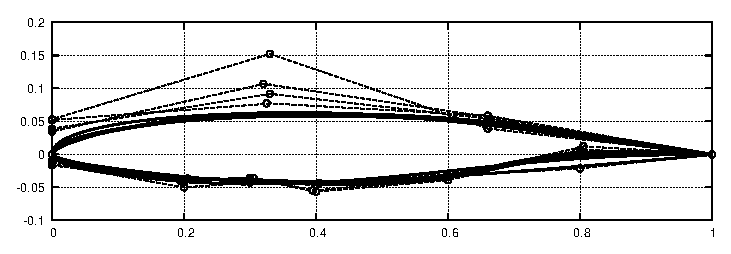
\includegraphics{thickness_s.eps}}
\end{minipage}
\caption{Design of a compressor cascade using KBD: Suction and pressure side thickness distributions and control point polygons for the four bases.} 
\label{CBRDtt}
\end{figure}


Four different optimization runs were performed in order to assess the effect of the KBD method both on EAs and the implementation of metamodels in MAEAs. The corresponding convergence plots are shown in fig.\ \ref{CBRDrela}. The use of metamodels in runs which do not rely upon the KBD method are not as efficient as expected. This is a caused by the use of an extended design space which is really necessary for being able to reproduce all four archived geometries. To demonstrate this, the four archived geometries are plotted together in figs.\ \ref{CBRDmm} and \ref{CBRDtt}. The large variance of the control points is more severe in the parameterization of the mean camber line (fig.\ \ref{CBRDmm}) regarding both coordinates and, also, in the thickness distribution along the suction side (fig.\ \ref{CBRDtt}). Using a more restricted design space would improve both the EA efficiency and the gain expected from the use of metamodels (MAEA) but could give suboptimal solutions if, by chance, the optimal geometry lays outside the design space. The comparison between EA and KBD-EA reveals the advantages of the proposed method (fig.\ \ref{CBRDrela}), since faster convergence is achieved. The comparison of KBD-MAEA with KBD-EA shows that the KBD method enhances the performance of the metamodel-based pre-evaluation phase. 

\begin{figure}[h!]
\begin{minipage}[b]{1\linewidth}
 \centering
 \resizebox*{12cm}{!}{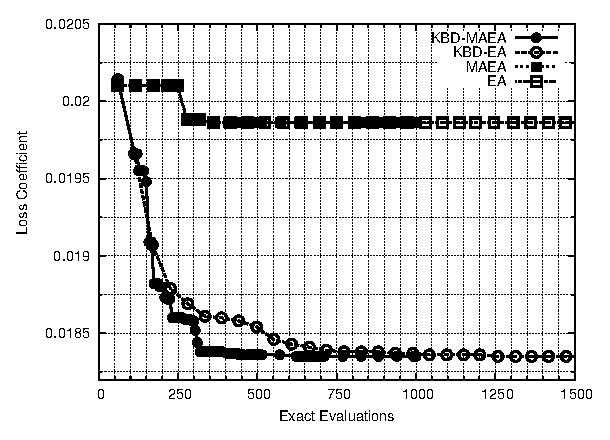
\includegraphics{Comp.eps}}
\end{minipage}
\caption{Design of a compressor cascade using KBD: Convergence comparison of four optimization runs using EA, KBD-EA, MAEA and KBD-MAEA. EA and MAEA have similar convergence plots, since the use of metamodels doesn't lead to extra gain, due to the extended range of the design variables. KBD-EA is significantly faster than  both EA and MAEA, thus proving the advantages of the proposed method. KBD-MAEA performs even better thanks to the positive effect of the proposed method on the use of metamodels.} 
\label{CBRDrela}
\end{figure}

The optimal blade resulting from the KBD-MAEA is presented in fig.\ \ref{CBRDrelaRes}. This design delivers $\omega\!=\!0.01834$ and $\Delta a\!=\!30.2^o$ at the desired flow conditions, outperforms any of the design-bases for the same flow-conditions and respects all the constraints. The airfoil designed using the KBD-MAEA is of significantly better quality compared with those delivered by the conventional runs, with or without the use of metamodels. 

\begin{figure}[h!]
\begin{minipage}[b]{1\linewidth}
 \centering
 \resizebox*{15cm}{!}{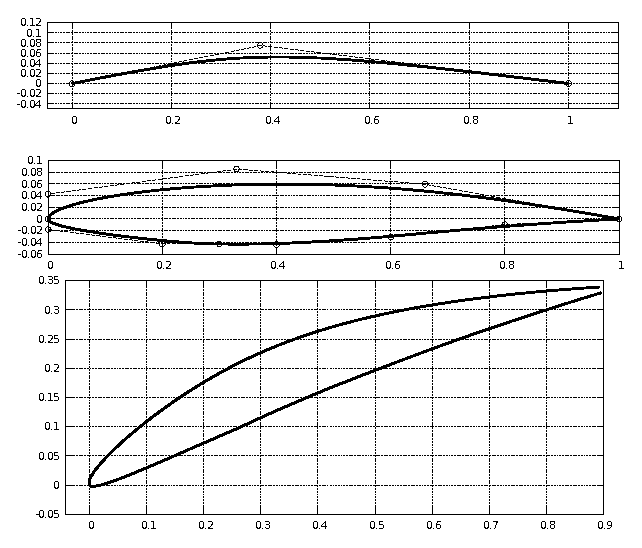
\includegraphics{ResD1.eps}}
\end{minipage}
\caption{Design of a compressor cascade using KBD: The optimal airfoil resulting from KBD-MAEA. Top: mean-camber line and thickness distributions together with their control polygons. Bottom: The airfoil shape after superimposing the thickness distribution on the mean-camber line and rotated at the desired stagger angle.} 
\label{CBRDrelaRes}
\end{figure}

%\begin{figure}[h!]
%\begin{minipage}[b]{1\linewidth}
% \centering
% \resizebox*{12cm}{!}{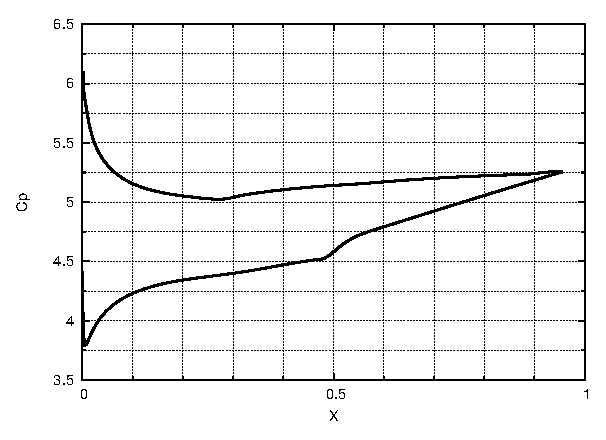
\includegraphics{Best_CP.eps}}
%\end{minipage}
%\caption{Pressure coefficient $C_p$ of the optimal airfoil fig.5\ref{CBRDrelaRes}.} 
%\label{CBRDrelaRes_cp}
%\end{figure}


%
% ---------------------------------------------------------------------------
% ----------------------- end of thesis sub-document ------------------------
% ---------------------------------------------------------------------------
					% KBD
% change according to folder and file names
\ifpdf
    \graphicspath{{4/figures/PNG/}{4/figures/PDF/}{3/figures/}}
\else
    \graphicspath{{4/figures/EPS/}{4/figures/}}
\fi

%: ----------------------- contents from here ------------------------
\chapter{EAs and MAEAs Driven by Principal Component Analysis} % top level followed by section, subsection
\label{VarCorrChapter}
%\begin{flushright}
%Any intelligent fool can make things  
%\linebreak
%bigger, more complex, and more violent. 
%\linebreak
%It takes a touch of genius, and a lot of  
%\linebreak
%courage, to move in the opposite direction.
%\linebreak
%Albert Einstein
%\end{flushright}

This chapter investigates the reasons for the drop in EAs or MAEAs efficiency used to solve ill-posed optimization problems \cite{Salomon,Roy_2002a,Ghisu_2010}, especially when these possess a great number N of design variables, and proposes techniques to overcome this unpleasant situation. Any degradation in the EAs or MAEAs efficiency reflects upon the number of evaluations (on the CFD software, for instance) required to reach the optimal solution(s).  Increasing the number of evaluations leads to longer optimization turn-around times and the routine application of EA-based optimization in large-scale industrial applications is, thus, hindered. The proposed methods adapt the application of the evolution operators accordingly and/or lead to the training of more dependable metamodels on patterns of properly reduced dimension (in case of MAEAs).

Modern industrial-scale optimization problems typically have several objectives and/or constraints with complex parameterization and a great number of design variables. The former is determined by the application under consideration whereas the latter is, often, ``inherited'' from the way experienced designers used to accomplish the same task in the past, without resorting to ``sophisticated'' optimization methods. From the practical point of view, a smooth transition to the EA-based optimization is necessary. Problems with several objectives and/or constraints which handle many design variables can easily become ill-posed, as discussed in section \ref{illpost}. The use of stochastic population-based search methods to solve ill-posed problems leads to excessively long computations, even on modern multi-processor platforms. Since the objectives and constraints are strictly defined by the application, the only way to increase the efficiency of EAs used to solve ill-posed optimization problems is via the appropriate handling of the parameterization. 

Changing the parameterization, though, may have a number of negative effects. First among them is that, in any industrial environment, a valuable amount of experience is embodied into the existing parameterization, in the sense that an experienced designer practically knows qualitatively what to change in order to achieve his/her goal; this would be lost by changing or modifying the parameterization scheme. Also, there is no guarantee that the new/altered parameterization, which must be built in accordance with the objectives so as to give a better-posed optimization problem, includes variables with clear interpretation (being, for instance, the coordinates of \Bezier\ control points, etc.). In fact, this is highly unlikeable. Any new parameterization, with unclear interpretation of the design variables, makes the accumulation of new experience impossible. Furthermore, in a specific project, the best parameterization depends on its correlation with the objectives and constraints. Therefore, a different parameterization would be necessary for any new design-optimization procedure, based on its objectives. To make things even worse, the best parameterization cannot be known in advance, since one should have the Pareto front available (in MOO problems) so as to extract the most appropriate parameterization (see below, in this chapter). All the above can be overcome by implementing the techniques proposed in this chapter.                 


As stated in \cite{Salomon}, standard GAs can find the global optimum in a number of widely used test functions due, not only to the efficiency of the recombination operator and the regular distribution of local minima, but also to the fact that the test functions are decomposable. Though \citep{Salomon} was based on GAs, its outcomes can be generalized to EAs. In \cite{Roy_2002a,Roy_2002b},  it was stated that ``real-life'' engineering design optimisation problems, as opposed to the widely used mathematical test cases, also involve ``interactions among design variables''. There, the notions of ``inseparable function interaction'' and ``variable dependency'' were introduced. The existence  of ``variable dependency'' poses a number of challenges in MOO algorithms which are similar to what is referred to as ill-posed optimization problems.
Also, as stated in \cite{Roy_2002b}, depending upon the nature of ``variable dependency'', additional features such as bias (non-linearity), multi-modality, deception and discontinuity may also occur and these will cause additional loss in the optimization algorithm efficiency. 


%  In \cite{Ghisu_2010}, the merits of adaptive parameterization in MOO with taboo search.



%In the same context with ill-posed optimization problems but with different phrasing significant work has been done by Ralf Salomon, Rajkumar Roy and Tiziano Ghisu. 
%Ralf Salomon presented, in \cite{Salomon}, the efficiency degradation of GAs if the same optimization problem was posed in a ``non-decomposable'' way. Later, Rajkumar Roy presented the, in \cite{Roy_2002a}, the notions of ``Inseparable Function Interaction'' and ``Variable Dependence''. Tiziano Ghisu, in \cite{Ghisu_2010}, presented the merits of adaptive parameterization in MOO with taboo search. 

 

\section{Ill-Posed Optimization Problems}
\label{illpost}
The two main reasons for increasing the number of calls to the evaluation software  required by an EA or MAEA, in order to locate the optimal solution(s), are: (a) the high number of design variables, $N\!>>$ and (b) the fact that an ill-posed optimization problem is solved. Needless to say that a high-dimensional ill-posed optimization problem is the worst case for an EA or MAEA.  Unfortunately, in practice, most engineering optimization problems share both features mentioned above . 

In EAs, the high number of design variables (N) results in efficiency loss. In the best case (well-posed problem), the cost for computing the optimal design(s) increases linearly with N. In MAEAs, the presence of $N\!>>$ design variables, apart from the way the optimal solution is approached (direct effect), impacts also the use of metamodels for which the training time and, mainly, their  prediction error increase noticeably. The loss in efficiency due to the ``less-accurate'' metamodel predictions (indirect effect) is, practically, superimposed to the performance degradation caused by the direct effect.  As a remedy to optimization problems with $N\!>>$, the KBD method was proposed in Chapter 3. From a completely different point of view, the KBD method reduces the problem dimension by exploiting the knowledge embodied into a small number of available archived designs and has already been presented and validated.             

On the other hand, ill-posed optimization problems are those dealing with (a) anisotropic and (b)  non-separable objective function/s $f(\vec{x})$. Note that (a) is a prerequisite for (b). In fact, ill-posed optimization problems are those dealing with non-separable objective functions. The definitions of anisotropic and non-separable functions follow in sections \ref{IllCon} and \ref{Nonsep}, respectively. Ill-posed problems, in combination with $N\!>>$, give rise to the so-called ``curse of dimensionality''. This stands for the situation in which the cost for solving an optimization problem increases superlinearly, instead of just linearly, with N. 
% Thus an ill-post optimization problem, when solved with EAs, is magnifying the negative effects of big N. 

%Herein the definitions of a) anisotropic objective function and b) non-separable objective function that characterize the objective function of an ill-posed problem are presented. Later, an investigation regarding the effects of ill-posed optimization problems on EA efficiency is carried out.  

\subsection{Anisotropic Objective Function}
\label{IllCon}
%The term anisotropic objective function refers to the condition were the contribution to the objective function value is largely anisotropic for the different design variables or ,more precisely, directions in search space.
An objective function $f(\vec{x})$, $\vec{x}=(x_1,...,x_N)$  is anisotropic with respect to $\vec{x}$ if it is differently affected by the same changes in the different components of $\vec{x}$. Though this thesis is dealing with non-gradient-based optimization methods, the anisotropy of f can be quantified by the variation of $\frac{\partial f}{\partial x_i}$ among the design variables $i$, close to the optimal solution. 

%This variation, and thus the magnitude of anisotropy, can be quantified via the condition number (a) of the Hessian matrix (H).


Let as assume that the convex-quadratic objective function
\begin{eqnarray}
   f(\vec{x}) = \frac{1}{2}\vec{x}^TH\vec{x}
   \label{conv.1}
\end{eqnarray}
where $H$ is a symmetric positive definite $N \times N$ matrix.
The variations in $\frac{\partial f}{\partial x_i}$  are expressed by the condition number a of matrix H. In such a case, $a$ is defined as the ratio of H's largest to smallest eigenvalue. 
These two eigenvalues correspond to the squared relative lengths of the principal axes of the ellipsoid $\vec{x}^TH\vec{x}\! =\! 1$. For points located along the principal axes, the gradient aligns with the axis itself and the ellipsoid-axis length determines the magnitude displacement in the design space required for obtaining a certain change in f. Therefore, f is said to be isotropic if the condition number of $H$ is $a=1$ (corresponding to a sphere or hyper-sphere-like isolines, see fig.\ \ref{illc}, left) and anisotropic if $a\!>>\!1$ (corresponding to an ellipse-like isolines, see fig.\ \ref{illc}, right).

  


\begin{figure}[h!]
\begin{minipage}[b]{1.0\linewidth}
 \centering
 \resizebox*{15cm}{!}{
\includegraphics{ellipseA.eps}}
\end{minipage}
%\begin{minipage}[b]{0.5\linewidth}
% \centering
% \resizebox*{7.5cm}{!}{
\includegraphics{ellipseA.eps}}
%\end{minipage}
\caption{Iso-value contours of an isotropic objective function with two design variables (left); the impact of $x_1$ and $x_2$ on f is the same. Iso-value contours of an anisotropic objective function, in which $x_2$ has greater impact on f than $x_1$ (right).} 
\label{illc}
\end{figure}

In practice, EAs are capable to efficiently deal with anisotropic objective functions without damaging their efficiency. If, however, the objective function is anisotropic and non-separable (see definition in section \ref{Nonsep}), the EA or MAEA is expected to perform less efficiently, unless a particular treatment is employed; such a treatment is proposed in this chapter.  

Furthermore, the anisotropy of f leads to the notion of more and less important design variables (or, in the case of non-separable f, more and less important directions in the design space). This piece of information can be used to reduce N, via the truncation of less important variables during the metamodel training phase, so as to increase its prediction ability.       


\subsection{Non-Separable Objective Function}     
\label{Nonsep}
The separability of an objective function $f:\vec{x}\mapsto f(\vec{x})$ is defined separately for each and every variable $x_i \in \vec{x}$. An objective function is said to be separable with respect to $x_i$ if the optimal value of $x_i$ does not depend on the value  any other design variable takes on. $f$ is said to be separable if and only if it is separable with respect to all components of $\vec{x}$.


\begin{figure}[h!]
\begin{minipage}[b]{1\linewidth}
 \centering
 \resizebox*{14cm}{!}{
\includegraphics{ellipseB.eps}}
\end{minipage}
%\begin{minipage}[b]{0.5\linewidth}
% \centering
% \resizebox*{9cm}{!}{\includegraphics{ellipseturn.eps}}
%\end{minipage}
\caption{Separable (left) and non-separable (right) objective functions.} 
\label{nonsep}
\end{figure}

As mentioned above, an ill-posed optimization problem suffers from the curse of dimensionality, the computational cost to solve it scales superlinearly with the number of design variables N. To better understand this, let us first examine a separable objective function. The cost for solving an optimization problem with a separable objective function increases linearly with N, since the global optimum can be located by minimizing $N$ objective functions with a single design variable each (separately minimise $f_i(x_i),~ \forall x_i \in \vec{x}$). Thus, the cost of solving a separable $N$-dimensional optimization problem is approximately $N$ times the cost of solving the equivalent 1D problem. On the other hand, this is not possible for an ill-posed optimization problem since, for at least one design variable, its optimal value depends on the values some or all of the other take on. Since the search space increases exponentially with N, this leads to a superlinear (with N) increase in the cost of solving ill-posed problems.   
 
\subsection{Investigation of EAs Efficiency Degradation in Ill-Posed Problems}
\label{Inv2}

In order to investigate the effects of ill-posed optimization problems on EA's efficiency, two mathematical test cases with different N values are solved, both in their separable (well-posed) and non-separable (ill-posed) form. The results presented in this section correspond to the mean performance of $10$ runs, with different random number generator seeds. 

The first analytical test case to be examined is a multi-dimensional ellipsoid (a 2D version of it can be seen in fig.\ \ref{nonsep}) described, in its separable form, by   


\begin{eqnarray}
   f(\vec{x})=\sum^{N}_{i=1} a^{\frac{i-1}{N-1}}x_i^2
   \label{ellipse} 
\end{eqnarray}
where the value of $a$ determines the anisotropy of the objective function. Large values of $a$ lead to increasingly anisotropic functions.

The same problem can be examined after casting it in non-separable form, as follows

\begin{eqnarray}
   f(\vec{y})=\sum^{N}_{i=1}a^{\frac{i-1}{N-1}}y_i^2
   \label{ellipse} 
\end{eqnarray}
where $\vec{y}=B\vec{x}$ and $B$ is an appropriate $N\times N$ orthogonal rotation matrix.

In order to investigate both the effects of the design space dimension ($N$) and the condition number ($a$), four different optimization problems were solved. A 10D ($N\!=\!10$) optimization problem was solved for $a\!=\!10$ and $a\!=\!100$,  fig. \ref{ellipse_t1}, and a $N\!=\!30$ problem for $a\!=\!100$ and $a\!=\!1000$, fig. \ref{ellipse_t2}. 


\begin{figure}[h!]
\begin{minipage}[b]{0.5\linewidth}
 \centering
 \resizebox*{7.5cm}{!}{\includegraphics{10_10d.eps}}
\end{minipage}
\begin{minipage}[b]{0.5\linewidth}
 \centering
 \resizebox*{7.5cm}{!}{\includegraphics{100_10d.eps}}
\end{minipage}
\caption{10D ellipsoid. Condition number $a\!=\!10$ (left). Condition number $a\!=\!100$ (right). Increasing $a$ from $10$ to $100$  increases the EAs performance gap between the separable and non-separable problems.} 
\label{ellipse_t1}
\end{figure}

\begin{figure}[h!]
\begin{minipage}[b]{0.5\linewidth}
 \centering
 \resizebox*{7.5cm}{!}{\includegraphics{100_30d.eps}}
\end{minipage}
\begin{minipage}[b]{0.5\linewidth}
 \centering
 \resizebox*{7.5cm}{!}{\includegraphics{1000_30d.eps}}
\end{minipage}
\caption{30D ellipsoid. Condition number $a\!=\!100$ (left).  Condition number $a\!=\!1000$ (right). As in the 10D case, increasing $a$ from $100$ to $1000$ causes additional losses in performance and increases the performance gap between separable and non-separable optimization problems.} 

\label{ellipse_t2}
\end{figure}

In figs. \ref{ellipse_t1} and \ref{ellipse_t2}, one may identify both the effects of increasing the condition number and increasing the problem dimension. A condition number with higher value leads to greater performance gap between the separable and non-separable cases, for both $N\!=\!10$ and $N\!=\!30$ cases. Increasing the problem dimension has the same effect. Focusing on the $a\!=\!100$ case, for both $N\!=\!10$ and $N\!=\!30$, one may observe that the difference in objective function values $|\Delta(f)|$, for the same computational cost of $9000$ evaluations, differ. For the $N\!=\!10$ case, $|\Delta(f)|\!=\!|f(non-separable)\!-\!f(separable)| \approx  10^{-4}$. On the other hand, for the $N=30$ case $|\Delta(f)| \approx  0.9$. This difference in $|\Delta(f)|$, between the 10D and 30D case, denotes a significant increase in the efficiency gap between separable and non-separable cases when the dimension is increased.      

The second analytical test case is concerned with the minimization of a multi-modal objective function described by  

\begin{eqnarray}
   f(\vec{x})=10N+(\sum^{N}_{i=1}x_i)^2 - 10N~ cos(\pi  \sum^{N}_{i=1}x_i)
   \label{mm} 
\end{eqnarray}

A 2D example is shown in fig.\ \ref{multimod}. As it appears in eq.\ \ref{mm}, the problem is non-separable. It can, though, easily be transformed to a separable one if $\vec{x}$ changes to $\vec{y}=B\vec{x}$, where $B$ is an appropriate rotation matrix.  A $45^o$ rotation is employed in each direction.  This objective function is extremely anisotropic since only one direction in the design space contributes to the objective function value and all the rest become irrelevant. Therefore, the condition number $a$ equals practically to $\infty$. This is an important class of objective functions since it resembles MOO problems as shown in section \ref{VCMM}.    

In order to investigate the effects of non-separability, as a function of the problems dimension, two optimization problems (5D and 30D) were solved.  
\begin{figure}[h!]
\begin{minipage}[b]{1\linewidth}
 \centering
 \resizebox*{14cm}{!}{\includegraphics{multimodnomap.eps}}
\end{minipage}
%\begin{minipage}[b]{1\linewidth}
 %\centering
 %\resizebox*{11cm}{!}{\includegraphics{multimodnomap.eps}}
%\end{minipage}
\caption{Minimization of eq. \ref{mm}, for N=2. The optimal value of $x_1$  depends on the choice of $x_2$ and vice-versa. So, this objective function is non-separable in terms of $x_1$ and $x_2$. Nevertheless, by aligning one of the two design variables with the $x_1\!=\!x_2$ axis, the problem becomes separable.} 

\label{multimod}
\end{figure}

In fig.\ \ref{multimodres}, it is demonstrated that both problems, if reformulated using  separable objective functions, outperform the non-separable ones. One may also observe that, the increase in problem's dimension causes an increase in efficiency gain, between separable and non-separable function cases. This conclusion is similar to the one made for the ellispoid test case. 



\begin{figure}[h!]
\begin{minipage}[b]{0.5\linewidth}
 \centering
 \resizebox*{7cm}{!}{\includegraphics{5d.eps}}
\end{minipage}
\begin{minipage}[b]{0.5\linewidth}
 \centering
 \resizebox*{7cm}{!}{\includegraphics{30d.eps}}
\end{minipage}
\caption{Solution of the 5D problem of eq.\ref{mm} (left). Solution of the 30D problem of eq.\ \ref{mm} (right). The loss in efficiency for problems with extremely anisotropic objective functions increases significantly with the design space dimension.} 
\label{multimodres}
\end{figure}

Through the preformed investigations  (figs. \ref{ellipse_t1}, \ref{ellipse_t2} and \ref{multimodres}), it is convincingly shown  that a significant amount of the EA efficiency can be lost when dealing with ill-posed optimization problems, especially when these are combined with high values of N. The degree of efficiency deterioration is proportional to three quantities:

\begin{description}
  \item[a)] The anisotropy magnitude: Increasing anisotropy leads to less efficient EAs (figs.\ \ref{ellipse_t1} and \ref{ellipse_t2}).    
  \item[b)] Function separability: Problems with separable objective functions with respect to their design variables can be solved significantly faster using EAs, as shown in figs.\ \ref{ellipse_t1}, \ref{ellipse_t2} and \ref{multimodres}.  
  \item[c)] The number of design variables $N$: It is obvious that, by increasing the number of design variables, any EA requires more computational resources to locate the optimal solution. Additionally, if combined with (b), the great value of $N$ leads to superlinear increase in cost (fig. \ref{multimodres}).  
\end{description}

\section{Ill-Posed MOO Problems}
\label{VCMM}
In ill-posed MOO problems, all comments made and conclusions reached must now be applied to the scalar cost function $\Phi$ (rather than the objective function f), since $\Phi$ is the quantity which ``drives'' the evolution operators. In MOO, ill-posed optimization problem are typically associated with functions $\Phi$ which are non-separable and extremely anisotropic. This results from the fact that a Pareto front of optimal non-dominated solutions is sought. Since the $\Phi$ values given to the population members depend upon the Pareto dominance, all members of the current front of non-dominated solutions have $\Phi\!=\!0$ (or very small values compared to the dominated members of the population if niching effects are taken into account). These leads to directions in the design space that have very small impact on $\Phi$, i.e.\ directions along the Pareto front ($\Phi\!\approx\!0$) and directions with high impact on it, i.e those perpendicular to the Pareto front, therefore, almost always, resulting in an extremely anisotropic problem. 

\section{Principal Component Analysis}
The aim is to find the appropriate transformation of the original set of variables $\vec{x}  \rightarrow \vec{x}^*$, capable to transform the ill-posed optimization problem in hand into a better-posed one. After this transformation, the objective function in SOO or  the scalar cost function $\Phi$ in MOO is expected to have enhanced separability properties with respect to the transformed design variables $\vec{x}^*$.  This procedure is equivalent to finding an orthogonal matrix $U$ ($UU^T=I$) and based on it, express $\vec{x}^*$ as $\vec{x}^*=U\vec{x}$. In this thesis, it is proposed that the topological characteristics of the Pareto front determine the appropriate transformation matrix $U$.  To extract these in a way which best represents the data variance, the Principal Component Analysis (PCA) method is used, \cite{Hayk1999,Jolliffe_2002}. The transformation matrix $U$ contains the Principal Directions (PDs) computed by the PCA applied to the members of the Pareto front.   

However, the Pareto front is the final goal of the optimization process and therefore, it is unknown during the optimization.  Instead, in the proposed method, in each EA generation, the front of non-dominated solutions (elite set) is the one undergoing PCA. This is a reasonable choice since, as the evolution proceeds, the current elite-set tends to the Pareto front. Thus, the PDs computed by processing the elite-set in each generation become progressively more reliable approximations of the PDs computed by analysing the Pareto front.

Applying PCA to the current elite-set calls for the transformation of  its members into a standardized data-set $X$, with $\mu=0$ and $\sigma=1$ in all directions. Next step is the computation of the empirical covariance matrix $P$, \cite{Fodor_2002, Jolliffe_2002},

\begin{equation} 
   P= \frac{1}{e}XX^T
   \label{Cov_Mat} 
\end{equation}
where $e$ is the size of the elite-set and $X$ the matrix formed using  the members of the elite-set as columns. Then, via the spectral decomposition theorem, \cite{Axler_1997, Fodor_2002}, $P$ can be written as

\begin{equation} 
   P= U\Lambda U^T
   \label{spectral}
\end{equation}
where $\Lambda\!=\!diag(\lambda_1 , . . . , \lambda_N )$ is a diagonal matrix with the eigenvalues of $P$ and $U$ is a $N\!\times\!N$ matrix containing the eigenvectors (PDs) as columns. 

\FloatBarrier
\section{The Welded Beam Case}

To better demonstrate the ill-posed nature of MOO problems, a modified version of the welded beam case \cite{coello2000use} is used, (fig.\ \ref{case}).  The minimization of both the cost ($K$) and the deflection ($\Delta$) of a welded beam subject to force $P$ (fig.\ \ref{case}) is desired. There are two design variables: the welding length ($x_1$ or $l$)  and the side length of the square cross section ($x_2$ or $t$). The design is subject to three constraints regarding shear stress ($\tau$), bending stress ($\sigma$) and buckling load ($P_c$).    


%\figuremacroW{case}{Welded beam case - Problem definition.}{In the examined case, design variables are square cross section side-length ($X_2 = t$) and welding length ($X_1 = l$) are the design variables.}{0.4}

The problem requires the minimization of both the cost
%\begin{equation} 
\begin{eqnarray}\nonumber
   K = 1.10471h^2l+0.04811t^2(14.0+l) %\\
%   = 1.10471h^2X_1+0.04811X_2^2(14.0+X_1)
   \label{Cost} 
\end{eqnarray}
and the deflection
%\end{equation}
\begin{eqnarray}
   \Delta = \frac{4PL^3}{Et^4} = \frac{4PL^3}{EX_2^4}
   \label{Deflection} 
\end{eqnarray}

\begin{figure}
\begin{minipage}[b]{1\linewidth}
 \centering
 \resizebox*{5cm}{!}{\includegraphics{case.eps}}
\end{minipage}
\caption{The Welded Beam Case: In the examined case, the welding length ($x_1\!=\!l$) and the square cross section side-length ($x_2\!=\!t$)  are the two design variables.} 
\label{case}
\end{figure}



The first constraint is related to the shear stress applied to the welding in order to ensure its structural integrity. The maximum shear stress depends on the type and quality of the welding.  This constraint is expressed as 
\begin{eqnarray}
   \tau = \sqrt{\tau_1^2 + \frac{\tau_1 \tau_2 l}{R} +\tau_2^2} \leq 13600 psi
\label{shear}
\end{eqnarray}
where
\begin{eqnarray}
   \nonumber \tau_1 = \frac{P}{\sqrt{2}hl}, ~~~\tau_2 = \frac{MR}{J}, ~~~M = P(L+\frac{l}{2}) 
\end{eqnarray}
\begin{eqnarray}
   \nonumber R = \sqrt{\frac{l^2}{4} + (\frac{h+t}{2})^2} 
\end{eqnarray}
\begin{eqnarray}
   \nonumber J = 2\left( \sqrt{2}hl\left( \frac{l^2}{12} + \left(\frac{h+t}{2}\right)^2 \right) \right)
\end{eqnarray}

The second constraint is on the bending stress applied to the beam, in order to ensure its structural integrity. The maximum bending stress depends on the beam material,
\begin{eqnarray}
   \sigma = \frac{6PL}{t^3} \leq 30000 psi
   \label{bend} 
\end{eqnarray}

Finally, in order to avoid buckling, the buckling load is also constrained as follows,  
\begin{eqnarray}
   P_c = \frac{4.013E\sqrt{\frac{t^8}{36}}}{L^2}\left( 1- \frac{t}{2L}\sqrt{\frac{E}{4G}} \right) \geq P 
   \label{back} 
\end{eqnarray}
where the welding height is $h \! = \!0.6 in$, the beam length is $L \! =\! 14 in$, the force is $P\! =\! 6000 lb$, the Young’s modulus is $E \!=\! 30 \! \times \! 10^6 psi$ and the shear modulus is $G\! = \!12 \! \times \! 10^6 psi$.  

Apart from the constraints which are related to structural integrity, two additional constraints, related to both objectives, were imposed. These are 
\begin{eqnarray}
   K \leq 50 \\
   \Delta \leq 0.25 
   \label{obj} 
\end{eqnarray}


%\begin{figure}[h!]
%\begin{minipage}[b]{0.5\linewidth}
% \centering
% \resizebox*{7cm}{!}{\includegraphics{Const_sx.eps}}
%\end{minipage}
%\begin{minipage}[b]{0.5\linewidth}
% \centering
% \resizebox*{7.5cm}{!}{\includegraphics{Const_tx.eps}}
%\end{minipage}
%\begin{minipage}[b]{0.5\linewidth}
% \centering
% \resizebox*{7.5cm}{!}{\includegraphics{Const_P.eps}}
%\end{minipage}
%\begin{minipage}[b]{0.5\linewidth}
% \centering
% \resizebox*{7.5cm}{!}{\includegraphics{Const_Price.eps}}
%\end{minipage}
%\begin{minipage}[b]{0.5\linewidth}
% \centering
% \resizebox*{7.5cm}{!}{\includegraphics{Const_Dx.eps}}
%\end{minipage}
%\begin{minipage}[b]{1\linewidth}
% \centering
% \resizebox*{12cm}{!}{\includegraphics{Const_ALL.eps}}
%\end{minipage}

%\caption{Investigation of the feasibility of the design $(X_1,X_2)$ plane. The overall feasible design space is presented in the lower right figure with white squares.} 
%\label{x1x2}
%\end{figure}

%This case was deliberately chosen as a demonstration case due to the clear physical meaning of the relations that appear between its design variables. By carefully examining the objectives it is clear that in order to decrease deflection $X_1$ must be increased(eq. \ref{Deflection}). However any increase in $X_1$ will lead to higher cost (eq. \ref{Cost} ). In order to keep cost stable $X_2$ must simultaneously decrease, this of-course is bounded by the structural constraints (eq. \ref{shear},\ref{bend} and \ref{back}). 
 
From the  $\Phi$ plot shown in fig.\ \ref{reco1} (left), it is evident that the problem in hand is both extremely anisotropic and non-separable (ill-posed). Using the proposed PCA of the elite-set (fig.\ \ref{reco1}, right) the computed PDs point to the directions in the design space which if used to define new design variables, would transform the ill-posed problem into a better-posed one. The direction with the largest eigenvalue $\lambda_1$ is the direction that describes the Pareto front is aligned with the $\Phi=0$ curve. On the other hand, the PD with the smallest eigenvalue $\lambda_2$ is the direction in the design space which corresponds to the largest change in $\Phi$ values. Smaller eigenvalue means smaller variance in the corresponding direction, in the elite-set. % Thus the EA, through its evolution operators, restricted the values of this direction within a small band of values denoting its importance regarding $\Phi$. 

%Looking at the physical meaning of the correlations between the design variables in the welded beam case; $e_1$ suggest that if one desires to move along the  $\Phi=0$ front he should either increase $X1$ (welding length) and decrease $X2$ (cross section) or vise vesra. In other words one can move from, say, expensive designs with small deflection to cheap designs with bigger deflection (fig.\ref{Pareto1}) by reducing the cross section but in order to keep respecting the various stress constraints (fig.\ref{x1x2}) one should simultaneously increase the welding length. On the other hand $e_2$ suggest that if one wants to move on the direction that would cause the biggest difference in $\Phi$ he should either increase or decrease both $X1$ \& $X2$ simultaneously.          

\begin{figure}[h!]
\begin{minipage}[b]{1\linewidth}
 \centering
 \resizebox*{!}{4.5 cm}{\includegraphics{DOFs.eps}}
\end{minipage}
%\begin{minipage}[b]{0.5\linewidth}
% \centering
%\resizebox*{8cm}{!}{\includegraphics{CaseCorr.eps}}
%\end{minipage}
\caption{The Welded Beam Case: Left; $\Phi$ iso-areas over the design space, at a specific generation during the evolution. Right; The elite-set, plotted in the design space. Based on it, two PDs denoted by $\lambda_1$ and $\lambda_2$ are computed.} 
\label{reco1}
\end{figure}

\begin{figure}[h!]
\begin{minipage}[b]{1\linewidth}
 \centering
 \resizebox*{!}{7 cm}{\includegraphics{Pareto.eps}}
\end{minipage}
\caption{The Welded Beam Case: The elite-set shown in fig.\ref{reco1} is plotted in the objective space, where $f_1$ = cost and $f_2$ = deflection.} 
\label{Pareto1}
\end{figure}


\section{PCA-Driven Evolution Operators} 
%The PCA driven evolution operators to better ``drive'' evolution by utilising the information about the design variable correlations are proposed here as a method to deal with ill-posed optimization problems. To be more specific, PCA is used to identify the relations in the form of direction in the design space. The design space is, then, temporarily aligned with these directions, the necessary evolution operators apply to the so--rotated space and, finally, the generated offspring are transformed back to the original design space. Any sort of dimensionality reduction or rotation of the design space occurs just before (and after) the application of the evolution operators. To initiate PCA, a small number of representative solutions to the problem must be available; this set is dynamically updated during the evolution. In MOO applications, this comprises the members of the current front of non--dominated solutions. In SOO problems, in which there is no set of non--dominated solutions, the principal components can be found by processing a user--defined number of top individuals in the current offspring population. It is evident that, as the evolution proceeds, and the current front of non--dominated solutions converges to the Pareto front, the principal components approach those of the Pareto front. 
In EA-based optimization, the application of the evolution operators may benefit a lot from the outcome of PCA, in order to reduce the computational cost required for the same quality of solutions. To be more specific, PCA is used to identify directions in the design space which, if used to define new optimization variables, would lead to an optimization problem with (almost) separable objective function. The design space is, then, temporarily aligned with the principal directions and the evolution operators apply to individuals expressed in the so-rotated axes. At the end of this phase, the generated offspring are transformed back to the original axes of the design space. The rotation of the design space axes occurs just before and after the application of the evolution operators thus deeming it transparent to the designer. To perform the PCA, a small number of well-performing solutions to the problem must be available. Herein, these are the members of the current elite-set, as stated before; this set is dynamically updated during the evolution. In MOO applications, the elite-set comprises the members of the current front of non--dominated solutions. In SOO problems, where the notion of dominality degenerates, the PDs  can be found by processing a user--defined number of the current top individuals. 

Let the aligned with the PDs design vectors \(\vec{x}_i\) be represented by \(\vec{x}^*_i\). The alignment is performed as follows
\begin{equation} 
   \vec{x}^*_i=U(\vec{x}_i-\vec{\mu}_{X})
   \label{align} %http://users.ics.tkk.fi/jhollmen/dippa/node30.html
\end{equation}
where $\vec{\mu}_{X}$ is the vector of mean (over the elite set) design variables.
The inverse transformation, from $\vec{x}^*_i$ to $\vec{x}_i$, is given by
\begin{equation} 
   \vec{x}_i=U^{-1}\vec{x}^*_i+\vec{\mu}_{X}
	\label{re-align}
\end{equation}
It should be stated that the CPU cost to compute \(U^{-1}\) is negligible since U is an orthogonal matrix and, thus, \(U^{-1} = U^T\). 

The two main PCA-driven evolution operators, recombination and mutation, are presented below.  

\paragraph{}
\subsection{PCA-Driven Recombination}
The recombination operator is applied to the rotated design variable-set which are sought to be as separable as possible. As shown in fig.\ \ref{reco2}, this changes the probability of the offspring appearance in the design space as if the problem was separable (fig.\ \ref{reco1}). 

\begin{figure}[h!]
\begin{minipage}[b]{0.5\linewidth}
 \centering
 \resizebox*{7cm}{!}{\includegraphics{SBX3dparents2a.eps}}
\end{minipage}
\begin{minipage}[b]{0.5\linewidth}
 \centering
 \resizebox*{7cm}{!}{\includegraphics{SBX3dparentsPCAa.eps}}
\end{minipage}
\caption{The Welded Beam Case: The  Offspring appearance probability using the SBX(n=0) recombination scheme (section \ref{RecombinationLabel}). Assume that there are two  parents shown by the two black dots. Left; SBX recombination. Right; PCA driven SBX recombination.} 
\label{reco2}
\end{figure}

From figs.\ \ref{reco1} and \ref{reco2}, it can be seen that the proposed method assigns higher offspring appearance probability to the regions near $\Phi\!=\!0$ which is the region that accommodates the currently best (elite) individuals. Therefore, the PCA-driven recombination  better achieves its goal of mixing, according to the building block hypothesis \cite{Gold89}. Mixing is the process in which building blocks (low-order schemata of high fitness) are combined to form new potentially fit schemata of higher order. The proposed method increases the probability individuals generated through the application of the recombination operator to be fit.   

%\begin{figure}[h!]
%\begin{minipage}[b]{1\linewidth}
% \centering
% \resizebox*{10cm}{!}{\includegraphics{ellipseturn_eig.eps}}
%\end{minipage}
%\caption{Example $\Phi'$ plot for} 
%\label{phi1}
%\end{figure}


\subsection{PCA-Driven Mutation}
Mutation is also applied to the design space aligned with the computed PDs. The mutation probability on each PD is dynamically updated based on the variance ($\vec{V}$) of the elite population members, projected onto the aforementioned direction ($V(i)$), eq. \ref{alignMut}. This is done in a way that keeps the overall mutation probability per individual constant (and equal to a user-defined value). The proposed method distributes the mutation probability among the PDs  in a way which is proportional to the importance of each direction, according to the characteristics of the current front of non-dominated solutions. As shown in the welded beam case, the importance of each PD, regarding either f (SOO) or $\Phi$ (MOO), is inversely proportional to its eigenvalue which quantifies the variance.  PDs  with high-valued eigenvalues receive smaller mutation probability, in contrast to the directions with low-valued eigenvalues which undergo mutation with higher probability. The formula used to adjust the mutation probability (per each newly computed direction (index $i$)) is        

\begin{equation}
	p_m^i = 0.1 p_m + \frac{0.9 p_m N}{D_V} \cdot \frac{V_{max}-V_i}{V_{max}-V_{min}} 
     \label{alignMut}
\end{equation}
where $p_m$ is a user--defined mutation probability,  
$V_{max}=\mbox{max}\{V_1,...,V_N\}$, $V_{min}=\mbox{min}\{V_1,...,V_N\}$ and 
\begin{equation}
	D_V=\sum_{i=1}^N \frac{V_{max}-V_i}{V_{max}-V_{min}}
\label{alignMut2} %http://users.ics.tkk.fi/jhollmen/dippa/node30.html
\end{equation}


%\begin{equation} 
%   P_m^{i}=0.1 P_m + \frac{0.9 P_m N}{P_m^{gl}} (1-\frac{(V_i-min(\vec{V}))}{(max(\vec{V})-min(\vec{V}))}),~~~~i=1,N 
%   \label{alignMut} %http://users.ics.tkk.fi/jhollmen/dippa/node30.html
%\end{equation}
%where $P_m$ is the user-defined mutation probability, N the number of design variables and 
%\begin{equation} 
%   P_m^{gl}=\sum^{N}_{i=1} 1-\frac{(V_i-min(\vec{V}))}{(max(\vec{V})-min(\vec{V}))}
%   \label{alignMut2} %http://users.ics.tkk.fi/jhollmen/dippa/node30.html
%\end{equation}



Let us denote  by $g$ the generation counter, by $k_{DB}$ the number of currently existing entries into the DB and by $k_{min}$ the minimum number of entries needed to initiate the use of the metamodel--based pre--evaluation phase. Then, the successive steps of the PCA--driven MAEA or MAEA(PCA) can be described as follows:
\begin{description}
  \item[Step 1:] For the current offspring population $S^{g}_\lambda$, set $\lambda^*\!=\!\lambda$ (if $k_{DB}\!<\!k_{min}$) or  $\lambda^*\!=\!\lambda_{e}$ (else), where $\lambda_{e}$ the number of offspring to be evaluated on the problem--specific evaluation software. 
  \item[Step 2:] If $k_{DB}\!\ge\!k_{min}$, $\lambda$ RBF networks are trained on paired input--output patterns selected from the DB, in the vicinity of each offspring. Pre--evaluate the $\lambda$ population members on the so--trained metamodels. Select the $\lambda_{ex}$ top of them, based on dominance and proximity criteria.
  \item[Step 3:] Evaluate the $\lambda_{e}$ offspring on the problem--specific evaluation software. Update $S^{g}_e$.
  \item[Step 4:] Compute the current set of PDs  based on the updated elite-set $S^{g}_e$ (eqs. \ref{Cov_Mat} and \ref{spectral}).
  \item[Step 5:] Align the design space with the so--computed PDs  (eq. \ref{align}). 
  \item[Step 6:] Create the new offspring population $S^{g+1}_\lambda$ through the application of the evolution operators to the aligned individuals. Re--align the generated offspring with the original design space coordinate system (eq.~\ref{re-align}).
  \item[Step 7:] Set $g\!\leftarrow\!g\!+\!1$; go to Step 1.
\end{description}
The above algorithm can readily be transformed to EA(PCA) by eliminating the use of metamodels or by setting $k_{min}$ to an ``infinite'' number.  
%\figuremacroW{MAEAPCA2}{MAEA-PCA}{Schematic representation of the PCA-driven MAEA algorithm.}{1.0}
%\begin{figure}[h!]
%\begin{minipage}[b]{1\linewidth}
% \centering
% \resizebox*{14cm}{!}{\includegraphics{MAEAPCA2.eps}}
%\end{minipage}
%\caption{Schematic representation of the PCA-driven MAEA algorithm.} 
%\label{MAEAPCA2}
%\end{figure}


%\figuremacroW{HypervolumeComparison}{Hypervolume Comparison}{Hypervolume comparison between EA and EA(PCA), metamodels where not used due to the fast evaluation time of The The The The The The The The The The Welded Beam Case: EA(PCA) outperforms traditional EA even though the dimensionality of the problem in hand is very low.}{0.9}

\subsection{Gain from the Use of EA(PCA)}

In order to demonstrate the performance gain from the use of the EA(PCA), the welded beam case and the two mathematical minimization problems already presented in section \ref{Inv2} are revisited. For each one of them, 10 runs were performed with different random number generator seeding. 

Regarding the two-objective welded beam problem, the average hypervolume indicator plotted in terms of the number of evaluations performed is presented in fig. \ref{HypervolumeComparison}. In this figure, it is shown that, even though the dimension of the problem was deliberately kept low ($N\!=\!2$) to facilitate the visual analysis of the obtained results, the gain from the use of the proposed method over the conventional EA is clear.  

\begin{figure}[h!]
\begin{minipage}[b]{1\linewidth}
 \centering
 \resizebox*{10cm}{!}{\includegraphics{HypervolumeComparison.eps}}
\end{minipage}
\caption{The Welded Beam Case: Average evolution of the hypervolume indicator using EA and EA(PCA). In this case, metamodels are not used due to the extremely small computational cost of each evaluation run. EA(PCA) outperforms traditional EA even though the dimensionality of the problem is very low.} 
\label{HypervolumeComparison}
\end{figure}



The comparison between conventional evolution operators and the PCA-driven ones, on the 30D non-separable ellipsoid with $a\!=\!1000$ (eq. \ref{ellipse}), is presented in fig.\ \ref{Ellt3}. This figure presents the mean objective function values of $10$ runs. 

\begin{figure}[h!]
\begin{minipage}[b]{1\linewidth}
 \centering
 \resizebox*{10cm}{!}{\includegraphics{1000_30d_pca.eps}}
\end{minipage}
\caption{30D non-separable ellipsoid with a=1000: Average convergence using EA and EA(PCA). The proposed PCA-driven evolution operators significantly outperform the conventional ones.} 
\label{Ellt3}
\end{figure}

In fig.\ \ref{Ellt3}, the significant gain from the use of the proposed EA(PCA) in comparison with an EA in the 30D ellipsoid case is shown.

Regarding the multi-dimensional and multi-modal problem of eq.\ \ref{mm} with N=30, a comparison between PCA-driven and conventional evolution operators is presented in fig.\ \ref{mmt3}.  In this figure, it is shown that the use of PCA-driven evolution operators significantly enhances the EA efficiency in the 30D multi-modal problem, too.


\begin{figure}[h!]
\begin{minipage}[b]{1\linewidth}
 \centering
 \resizebox*{10cm}{!}{\includegraphics{30d_pca.eps}}
\end{minipage}
\caption{30D multi-modal problem: Average convergence using the EA and the EA(PCA). Similar to fig.\ \ref{Ellt3}, the proposed PCA-driven evolution operators significantly outperform the traditional ones.} 
\label{mmt3}
\end{figure}


%\FloatBarrier
\section{EAs Assisted by PCA-Driven Metamodels}
In MAEAs, the main challenge regarding the use of artificial neural networks as metamodels is to overcome the so--called curse of dimensionality in problems with a large number of design variables. 
The number of training patterns required to build a reliable metamodel increases with N; a side--effect is that their training becomes computationally costly. On the other hand, the need for more training patterns per metamodel delays the commencement of the IPE phase during the MAEA, until the DB collects a substantial number of entries. This leads to a further increase in the wall clock time of the optimization run.

This thesis proposes the reduction in the number of the RBF network sensory (input) nodes and, consequently, the required number of training patterns. The eigenvectors computed through the PCA of the elite-set are associated with the objective function variance. 
If the elite-set is expressed in a coordinate system aligned with the PDs, it is expected that any plot of the objective function (SOO) or $\Phi$ (MOO) in terms of the first components (i.e. those with the highest variance) must be scattered enough. In contrast, along the PDs with small variances, the elite members are much less scattered. 

The proposed method takes advantage of the above and cuts off a pre-selected number of the RBF network sensory units, particularly those related to the highest variance directions in the design space. As a result, the RBF networks are trained on lower dimension data. 
This truncation is applied only during the RBF network training, by firstly rotating/aligning all the selected training patterns with the computed PDs and, then, cutting those sensory nodes which correspond to the highest eigenvalues off. The number of the components to be cut off is user-defined.
    
% The use of the IPE technique, in its standard form, would require the use of RBF networks with two sensory nodes each, trained on neighbouring to the candidate solution, already evaluated stored individuals as shown in figure \ref{2dann}. 
    
    
%\begin{figure}[h!]
%\begin{minipage}[b]{1\linewidth}
% \centering
% \resizebox*{15cm}{!}{\includegraphics{2dANN.eps}}
%\end{minipage}
%\caption{Welded beam test problem: ANN with two sensory node used as metamodel in the standard IPE form. The ANN prediction is plotted as a surface grid and the training patterns used for its training as dots.} 
%\label{2dann}
%\end{figure}

\begin{figure}
\begin{minipage}{0.48\textwidth}
\includegraphics[scale=1.2]{IPE/x1_x2.eps}
\end{minipage}
\begin{minipage}{0.48\textwidth}
\includegraphics[scale=1.2]{IPE/f1_f2.eps}
\end{minipage}
\caption{The Welded Beam Case: An instant of the evolution process, where the current elite set, a candidate solution (A) and the training patterns selected from the current DB for training the metamodel to be used to predict the objective function value at A are plotted in the design (left) and objective (right) space.}
\label{fig:f1f2}
\end{figure}

Fig.\ \ref{fig:f1f2} presents an instant of the evolution process, at the end of the $6^{\mbox{th}}$ generation of one of the runs. At this instant, $\lambda$ new offspring have just been generated. Let us assume that the candidate solution A, with $(x_1, x_2)\!=\!(0.2,0.5)$  shown in fig.\ \ref{fig:f1f2}, needs to be pre-evaluated using an appropriately trained local RBF network. 
For this purpose, $19$ patterns are selected from the DB using the standard selection procedure. 
In fig.\ \ref{fig:f1f2}, the training patterns, the candidate solution and, also, the current elite-set are plotted both in the design ($x_1, x_2$) and objective ($f_1, f_2$) spaces. 
The exact values of $f_1$ and $f_2$ for A are also shown.
It is evident that, in a problem with only two design variables, there is no reason to reduce the number of design variables during the training of the RBF networks. However, it was decided to do so, just for the purpose of demonstration.  

\begin{figure}
\begin{minipage}{0.48\textwidth}
\includegraphics[scale=1.2]{IPE/f1_x1.eps}
\end{minipage}
\begin{minipage}{0.48\textwidth}
\includegraphics[scale=1.2]{IPE/f1_x2.eps}
\end{minipage}
\caption{The Welded Beam Case: RBF network predictions of $f_1$ if $x_1$ (left) and $x_2$ (right) are separately applied to the single sensory unit of the network. }
\label{fig:f1x1x2}
\end{figure}

\begin{figure}
\begin{minipage}{0.48\textwidth}
\includegraphics[scale=1.2]{IPE/f2_x1.eps}
\end{minipage}
\begin{minipage}{0.48\textwidth}
\includegraphics[scale=1.2]{IPE/f2_x2.eps}
\end{minipage}
\caption{The Welded Beam Case: RBF network predictions of $f_2$ if $x_1$ (left) and $x_2$ (right) are separately applied to the single sensory unit of the network. }
\label{fig:f2x1x2}
\end{figure}

A first demonstration of the proposed method is based on the welded
beam problem (fig.\ \ref{case}). In fig.\ \ref{fig:f1x1x2}, the $f_1$ predictions using two RBF networks, with either $x_1$ or $x_2$ as the only sensory unit of each network, are shown. Though these networks, after being trained on the selected $19$ patterns, must be used to predict the objective functions only at A, it is interesting to observe the overall deviation between the continuous line which stands for the network response and the training patterns' responses. 
Recall that the number of RBF centers is less than the number of training parameters, so the network does not interpolate the training patterns.
The observed high deviations, which could be even higher for some other candidate solutions, are easily explained by the fact that a two-variable function $f_1(x_1,x_2)$ is handled as $f_1(x_1)$ or $f_1(x_2)$. The corresponding results for $f_2$, instead of $f_1$, are shown in fig.\ \ref{fig:f2x1x2}. 
The exact objective function values at A along with the RBF predictions are tabulated in table \ref{tab:f1f2x1x2}. It can be seen that $f_1$ is predicted with a relative error of  $\approx \! 57\%$ if $f_1\!=\!f_1(x_1)$ and $\approx \! 138\%$ if $f_1\!=\!f_1(x_2)$ and the error of $f_2$ is  $\approx \! 110\%$ if $ f_2\!=\!f_2(x_1)$ and $\approx \! 260\%$ if $ f_2\!=\!f_2(x_2)$.


\begin{figure}
\begin{minipage}{0.48\textwidth}
\includegraphics[scale=1.2]{IPE/f1_e1.eps}
\end{minipage}
\begin{minipage}{0.48\textwidth}
\includegraphics[scale=1.2]{IPE/f1_e2.eps}
\end{minipage}
\caption{The Welded Beam Case: RBF network predictions of $f_1$ if $e_1$ (left) and $e_2$ (right) are separately applied to the single sensory unit of the network.}
\label{fig:f1e1e2}
\end{figure}

\begin{figure}
\begin{minipage}{0.48\textwidth}
\includegraphics[scale=1.2]{IPE/f2_e1.eps}
\end{minipage}
\begin{minipage}{0.48\textwidth}
\includegraphics[scale=1.2]{IPE/f2_e2.eps}
\end{minipage}
\caption{The Welded Beam Case: RBF network predictions of $f_2$ if $e_1$ (left) and $e_2$ (right) are separately applied to the single sensory unit of the network. }
\label{fig:f2e1e2}
\end{figure}

\begin{table}[h!]
\begin{center}
\begin{tabular}{c  c | c | c}
		&      Exact  	 		&  RBF network predictions    &  RBF network  predictions   \\
		&  $(f_1,f_2)$ values   &  assuming $f_i=f_i(x_1)$    &   assuming $f_i=f_i(x_2)$  \\
		\hline
$f_1$	& $28.07$   &      $11.88$     &      $66.9$        \\
$f_2$	& $0.73$     &      $-0.08$     &      $2.66$        \\
\end{tabular}
\end{center}
\caption{The Welded Beam Case: Exact response and RBF network predictions of $f_1$ and $f_2$ at A, using either $x_1$ or $x_2$ as the only input to the network.}
\label{tab:f1f2x1x2}
\end{table}


The PCA of the current elite-set is used to compute the two PDs which, in turn, are used to select the single variable that must preferably be associated with the only sensory unit of the RBF network. The design space is transformed according to the computed PDs and the RBF network training is repeated using either $e_1$ or $e_2$, instead of $x_1$ and $x_2$, as input. 
The RBF networks' predictions are shown in fig.\ \ref{fig:f1e1e2} and \ref{fig:f2e1e2} and table \ref{tab:f1f2e1e2}. 
In particular, $f_1$ is predicted with a relative error of $\approx \! 17\%$ if $f_1\!=\!f_1(e_1)$ and $\approx \! 13\%$ if $f_1\!=\!f_1(e_2)$ and $f_2$ with $\approx \! 41\%$ if $f_2\!=\!f_2(e_1)$ and $\approx \! 43\%$ if $f_2\!=\!f_2(e_2)$. From these figures, it is concluded that the RBF networks can be trained only on $e_2$, i.e. the PD with the smaller variance, since the training patterns are less scattered both in ($e_2,f_1$) and ($e_2,f_2$) and the obtained prediction is more dependable.




\begin{table}[h!]
\begin{center}
\begin{tabular}{c  c | c | c}
		&      Exact  	 		&  RBF network predictions    &  RBF network  predictions   \\
		&  $(f_1,f_2)$ values   &  assuming $f_i=f_i(e_1)$    &   assuming $f_i=f_i(e_2)$  \\
		\hline
$f_1$	& $28.07$   &      $32.86$     &      $31.84$        \\
$f_2$	& $0.73$     &      $ 1.04$     &       $ 1.06$        \\
\end{tabular}
\end{center}
\caption{The Welded Beam Case: Exact responses and RBF network predictions of $f_1$ and $f_2$ at A, using either $e_1$ or $e_2$ as the only input to the network.}
\label{tab:f1f2e1e2}
\end{table}


%stelios 
\subsection{Gain from the Use of M(PCA)AEA(PCA)}

To demonstrate the gain in performance from the use of the proposed PCA-assisted metamodels, 10 runs using the so-called M(PCA)AEA(PCA) optimization for the two mathematical test cases presented in section \ref{Inv2} were performed with different random number generator seeding.  

The comparison between  runs based on the use of conventional metamodels where PCA is used only to drive the evolution operators (denoted by MAEA(PCA)) and additionally enhanced with PCA-assisted metamodels  or M(PCA)AEA(PCA), for the 30D non-separable ellipsoid function with $a=1000$ (eq. \ref{ellipse}), is presented in fig. \ref{Ellt3-m}. The plots refer to the mean objective function values of $10$ runs. The IPE phase for the MAEA(PCA) initiated after $300$ individuals were stored in the DB and $25$ to $29$ training patterns, in the $30D$ space, were used to train the RBF networks employed as metamodels. Regarding the M(PCA)AEA(PCA), the IPE phase started after only the first $100$ individuals were stored in the DB since only $4$ to $8$ training patterns, in the truncated  $10D$  space, were required for the RBF network training. In the latter case, the RBF networks were trained on the $10$ most important directions in the design space, as identified by the PCA. 

\begin{figure}[h!]
\begin{minipage}[b]{1\linewidth}
 \centering
 \resizebox*{10cm}{!}{\includegraphics{1000_30d_pca_ipe.eps}}
\end{minipage}
\caption{30D non-separable ellipsoid with a=1000: Average convergence of EA(PCA), MAEA(PCA) and M(PCA)AEA(PCA). The proposed M(PCA)AEA(PCA) outperforms both of the other variants.} 
\label{Ellt3-m}
\end{figure}


Regarding the multi-dimensional and multi-modal test case of eq.\ref{mm}, a comparison regarding EA(PCA), MAEA(PCA) and M(PCA)AEA(PCA) is presented, for the 30D  problem, in fig.\ref{mmt3m}. Regarding the MAEA(PCA), the  IPE phase initiated after $300$ individuals were stored in the DB and $15$ to $19$ training patterns in the $\Re^{30}$ space were used to train the  metamodel. Regarding M(PCA)AEA(PCA), the training pattern dimension was truncated from $30$ to the $10$ most important ones with respect to f. This allowed for the  IPE phase to start just after only $100$ individuals were stored in the DB, since only $5$ to $9$ training patterns were required for the RBF network training.

\begin{figure}[h!]
\begin{minipage}[b]{1\linewidth}
 \centering
 \resizebox*{11cm}{!}{\includegraphics{30d_pca_ipe.eps}}
\end{minipage}
\caption{30D multi-modal problem: Average convergence of EA(PCA), MAEA(PCA) and M(PCA)AEA(PCA).The proposed M(PCA)AEA(PCA) method performs much better than the other variants.} 
\label{mmt3m}
\end{figure}

In figs. \ref{Ellt3-m} and \ref{mmt3m}, one may observe that the use of PCA-driven metamodels further enhances the MAEA efficiency.

%stelios

\section{Design of a Compressor Cascade}


The design of a 2D compressor cascade operating at $M_1\!=\!0.54$, $a_1\!=\!44^o$ and $Re\!=\!4\times10^5$ for minimum total pressure losses coefficient $\omega$ (eq.\ \ref{omegaLosses}) is sought. 

The blade airfoil is designed subject to a number of aerodynamic and geometrical constraints: the optimal airfoil must turn the flow by more than $30^o$ and the blade airfoil thickness at three chord-wise positions $0.3c$, $0.6c$ \& $0.9c$ must be greater that $0.10c$, $0.08c$ \& $0.01c$,  respectively.     

The airfoil shape is parameterized based on its mean-camber line and super-imposed thickness distributions, presented in section \ref{Drela1}, yielding $27$ design variables.

The advantages of using the M(PCA)AEA(PCA) method can be seen by comparing the performances of a conventional MAEA and the M(PCA)AEA(PCA). In both cases, the populations are $\mu\!=\!20$, $\lambda\!=\!60$ and $\lambda_e\!=\!6$. Both cases used local RBF networks as metamodels trained on a small number of automatically selected patterns. The MAEA used a number of  $20$ to $30$ training patterns in the $27D$ space. The IPE phase for the MAEA started after $400$ individuals were stored in the DB. Regarding M(PCA)AEA(PCA), the RBF networks used as metamodels were trained on $5$ to $8$ patterns in the  $10D$ space. The reduced dimension made the earlier use of metamodels possible; in the M(PCA)AEA(PCA) run, the IPE phase started after the first $200$ individuals were stored in the DB. 


\begin{figure}[h!]
\begin{minipage}[b]{1\linewidth}
 \centering
 \resizebox*{11cm}{!}{\includegraphics{CompConv_1.eps}}
\end{minipage}
\caption{Design of a compressor cascade:  Comparison of the mean value and standard deviation from  $10$ independent runs performed using MAEA, MAEA(PCA) and M(PCA)AEA(PCA).} 
\label{PCADrelaRes}
\end{figure}

Fig. \ref{PCADrelaRes} shows the convergence of both methods. M(PCA)AEA(PCA) outperforms the conventional MAEA, during all but the early generations of the optimization procedure. 

\begin{figure}[h!]
\begin{minipage}[b]{1\linewidth}
 \centering
 \resizebox*{16cm}{!}{\includegraphics{ResD.eps}}
\end{minipage}
\caption{Design of a compressor cascade: The optimal airfoil resulted from M(PCA)AEA(PCA). Left: mean-camber line and thickness distribution together with their control polygons. Right: The final airfoil after superimposing thickness distributions on the mean camber line and turned to the fixed stagger angle.} 
\label{PCADrelaRes}
\end{figure}

The optimal airfoil resulting from M(PCA)AEA(PCA) run, shown in fig. \ref{PCADrelaRes}, has a total pressure loss coefficient value of $\omega=0.01803$ and respects both the thickness and flow turning constraints.  The flow turning of the optimal blade is $\Delta a=30^o$.

\begin{figure}[h!]
\begin{minipage}[b]{1\linewidth}
 \centering
 \resizebox*{10cm}{!}{\includegraphics{Best_CP_PCA.eps}}
\end{minipage}
\caption{Design of a compressor cascade: Pressure coefficient $C_p$ of the optimal airfoil shown in fig. \ref{PCADrelaRes}.} 
\label{PCADrelaRes_cp}
\end{figure}

% ---------------------------------------------------------------------------
% ----------------------- end of thesis sub-document ------------------------
% ---------------------------------------------------------------------------					% PCA
% change according to folder and file names
\ifpdf
    \graphicspath{{5/figures/PNG/}{5/figures/PDF/}{4/figures/}}
\else
    \graphicspath{{5/figures/EPS/}{5/figures/}}
\fi

%: ----------------------- contents from here ------------------------
\chapter{Optimization of Hydraulic Turbomachines} % top level followed by section, subsection
%\begin{flushright}
%%Water is for turbines.   
%The Wise Find Pleasure in Water
%\linebreak
%Confucius
%\linebreak
%\end{flushright}

In this chapter, the KBD method presented in Chapter \ref{KBDchapter} and the MAEA which is further driven by the principal component analysis (PCA) of promising individuals, presented in Chapter \ref{VarCorrChapter}, are used to solve large scale industrial problems related to the design-optimizations  of hydraulic turbines. 

In order to perform a successful optimization, a reliable evaluation procedure must be available. The evaluation procedure used in this chapter (fig. \ref{evaltool}) comprises three parts: the parameterization tool which is able to generate 3D turbine blade shapes, the grid generation tool able to automatically generate computational grids in any geometry created according to the aforementioned paremeterization tool and the CFD software. Section \ref{ParamEval} presents the basic features of the aforementioned tools. Section \ref{Paramt} is about the  parameterization  which is appropriate for 3D geometries of any type of reaction turbines. The grid generation is presented in section \ref{SpaceDisct}. And, finally, the Euler solver used to predict the water flow through the flow passage is presented in section \ref{FlowSolvert}.

\begin{figure}[h!]
\centering
\includegraphics[width=135mm]{Optimizationloop.eps} 
\caption{According to the EASY nomenclature, the evaluation of each new candidate solution created during the evolution starts by reading the corresponding values of the design variables from the ``task.dat" file. A series of codes, being I/O compatible, are sequentially used to, finally, create the ``task.res" and ``task.cns" files which include the objective and constraint function values, respectively. The evaluation process is considered to be terminated once the ``task.res" and ``task.cns" files  become available to the search engine of EASY. The names of the executable files required for a single evaluation are listed in the script file "task.bat". }
\label{evaltool}
\end{figure}      


Post-processing is an indispensable part of the evaluation procedure. Post-processing tools are used to compute the metrics associated with the fitness of each candidate solution, as presented in section \ref{metrics}. 

Two problems are examined. The first problem is  dealing with the design-optimization of a Francis turbine runner to be installed in a pre-existing hydroelectric plant. This case is mainly used to study the gain from the use of the developed KBD method (Chapter \ref{KBDchapter}), as compared with the conventional EA, in an industrial environment where archived past designs, i.e. the outcomes of more or less similar projects, are, in fact, available.

The second problem is related to the design of a new type of hydraulic turbines, the so-called Hydromatrix$\circledR$. This case is used to demonstrate the gain from the implementation of the PCA-driven evolution operators (MAEA(PCA)), as compared with standard MAEA.     

      
\section{Evaluation Procedure}
\label{ParamEval}
\subsection{Parameterization for Turbine Blades}
\label{Paramt}
The  parameterization of a hydraulic turbine blade, of axial radial or mixed flow type, consists of two steps. The first step is the parameterization of its 3D mean-camber surface. The second step is concerned with the thickness of the blade which is defined by the airfoil shape and the thickness distribution across the blade, \cite{dipl_livia,dipl_simon}.

Starting point of the parameterization of the mean-camber surface is its meridional projection. The meridional projection of the mean-camber surface is confined by 4 curves, namely the hub and shroud generatrices, the leading and trailing edge curves (fig.\ \ref{param1}). All four curves are parameterized by a user-defined number of \Bezier\ control points.


%\begin{figure}[h!]
%\centering
%\includegraphics[width=100mm]{param1.eps} 
%\caption{Example of a meridional surface (here a Matrix blade) in cylindrical coordinates (r,z,f=0)}
%\label{param1}
%\end{figure}

Having defined the meridional projection of the mean-camber surface,  the generation of the 3D shape of the mean-camber surface follows. A set of 2D iso-span lines, distributed between the shroud and hub,  are generated (fig.\ \ref{param1}). The 3D shape of the aforementioned lines is  based on their meridional projection and a number of parameters, namely $\rho,\theta,\beta,\zeta$ and $\mu$, which are all defined below. These 3D lines are, then, used as the skeleton of the blade mean-camber surface (fig.\ \ref{param3}).

\begin{figure}[h!]
\begin{minipage}[b]{0.5\linewidth}
 \centering
 \resizebox*{6.5cm}{!}{\includegraphics{param1.eps}}
\end{minipage}
\begin{minipage}[b]{0.5\linewidth}
 \centering
 \resizebox*{6.5cm}{!}{\includegraphics{param2.eps}}
\end{minipage}
\caption{Left: Meridional projection of the mean-camber surface of a Hydromatrix$\circledR$ blade. Right: The 2D iso-span lines distributed between shroud and hub. Definition of $\rho$ for the leading and trailing edge.}
\label{param1}
\end{figure}
 

%\begin{figure}[h!]
%\centering
%\includegraphics[width=100mm]{param2.eps} 
%\caption{Example of a 2-dimensional streamlines distribution between shroud and hub (here 11 streamlines). %Definition of $\rho$.}
%\label{param2}
%\end{figure}

The $\rho$ value is defined at each point along both the leading (LE) and trailing (TE) edges as the normalized meridional projection of the arc-length of the edge, with zero value at shroud and unit value at hub (fig.\ \ref{param1}). 

\begin{figure}[h!]
\centering
\includegraphics[width=120mm]{param3.eps} 
\caption{The 3D iso-span lines and their superimposed thickness profiles.}
\label{param3}
\end{figure}

The angular position of the LE and TE is controlled by the so-called wrap-around angle $\theta$. % is defined as the angle between the projected linear connection of a mean-surface-point and the z-axis onto the x-y-plane and the x-axis.
$\theta(\rho)$ distributions for the LE and TE together with the r and z values of their meridional projections define the final 3D shape of both edges. On the other hand, $\beta$ is defined as the angle between the local tangent to the mean-camber surface and the tangent to the z-centered circle through this point. Therefore, the $\beta(\rho)$ distributions define the mean-camber surface metal angles throughout the previously defined LE and TE. $\beta(\rho)$ and $\theta(\rho)$ distributions are parameterized as \Bezier\ curves of a user-defined degree (fig.\ \ref{param4}).  


\begin{figure}[h!]
\begin{minipage}[b]{1\linewidth}
 \centering
 \resizebox*{14cm}{!}{\includegraphics{param4_5.eps}}
\end{minipage}
%\begin{minipage}[b]{0.5\linewidth}
% \centering
% \resizebox*{6.5cm}{!}{\includegraphics{param5.eps}}
%\end{minipage}
\caption{Left: $\beta(\rho)$ distribution. Right: $\theta(\rho)$ distribution.}
\label{param4}
\end{figure}

The final step in the parameterization of the mean-camber surface is to define its shape between the LE and TE for all the iso-span lines. This is achieved through the conformal mapping $\Phi$


\begin{equation} 
   \Phi:(r,z)\rightarrow \mu, ~~~~\mu=\int{\frac{1}{r}dl}
   \label{phi1} 
\end{equation}
where $l$ denotes the arc-length of the meridional projection of the iso-span line. This conformal mapping performs the angle-preserving transformation of the iso-span lines from the cylindrical  $(r,z,\theta)$ to the $(\mu,\theta)$ coordinate system. The iso-span lines (in the $(\mu,\theta)$ coordinate system) are defined by third-degree \Bezier\ curves. The first and last control points are fixed on the LE and TE points of each iso-span line and the two internal control points depend on $\zeta_{LE}, ~\zeta_{TE}, ~\beta_{LE}$ and $\beta_{TE}$ angles, respectively (fig.\ \ref{param7}).
  
Finally, the two $\zeta(\rho)$ distributions, for the LE ($\zeta_{LE}$) and TE ($\zeta_{TE}$), define the position of the two internal control points for all the iso-span lines ($0\leq\rho\leq1$). Therefore, the $\zeta$ distributions can be seen as the curvature control system of the aforementioned parameterization of the mean-camber surface scheme, since it defines how strongly the $\beta$ values at LE and TE affect the $\beta$ values in the interior of the mean-camber surface. Similar to $\theta(\rho)$ and $\beta(\rho)$, the $\zeta(\rho)$ distributions are also parameterized as \Bezier\ curves of a user-defined degree (fig.\ \ref{param7}). Then the  inverse conformal mapping $\Phi^{-1}$ is used to transform the iso-span lines from the $(\mu,\theta)$ coordinate system back to the cylindrical one. 

\begin{figure}[h!]
\begin{minipage}[b]{1\linewidth}
 \centering
 \resizebox*{14cm}{!}{\includegraphics{param6_7.eps}}
\end{minipage}
%\begin{minipage}[b]{0.5\linewidth}
% \centering
% \resizebox*{7.5cm}{!}{\includegraphics{param7.eps}}
%\end{minipage}
\caption{Left: $\zeta(\rho)$ distributions for $\zeta_{LE}$ and $\zeta_{TE}$. Right: Iso-span line, in the $(\mu,\theta)$ coordinate system, and its \Bezier\ control point polygon.}
\label{param7}
\end{figure}

The airfoil profiles are defined by a user-defined number of \Bezier\ points (fig.\ \ref{param8}) and the absolute thickness by two thickness (t($\rho$)) distributions (fig.\ \ref{param10}) (separately for the SS and PS). The airfoil profiles are scaled so that their maximum thickness be equal to the one specified by the t($\rho$) distribution. Finally, the scaled airfoil profiles are superimposed onto the mean-camber surface to create the final 3D blade (fig.\ \ref{param10}).  

\begin{figure}[h!]
\centering
\includegraphics[width=150mm]{param8.eps} 
\caption{\Bezier\ control polygons for the PS and SS.}
\label{param8}
\end{figure}

%\begin{figure}[h!]
%\centering
%\includegraphics[width=60mm]{figure5.eps} 
%\caption{thickens-$\rho$ distribution.}
%\label{param9}
%\end{figure}


\begin{figure}[h!]
\begin{minipage}[b]{0.5\linewidth}
 \centering
 \resizebox*{6.5cm}{!}{\includegraphics{param9.eps}}
\end{minipage}
\begin{minipage}[b]{0.5\linewidth}
 \centering
 \resizebox*{6.5cm}{!}{\includegraphics{param10.eps}}
\end{minipage}
\caption{Left: t($\rho$) distribution. Right: 3D geometry of a Hydromatrix$\circledR$ turbine with three blades.}
\label{param10}
\end{figure}

\FloatBarrier
\subsection{Space Discretization - Grid Generation}
\label{SpaceDisct}
A multi-block structured grid generator, tailor-made for hydraulic turbomachines, which has been developed by Andritz-ASROE is used. This is able to handle axial, radial and mixed flow machines. Structured grids, using blocks with fixed topology can, via stretching and twisting, create grids which fit the geometries under consideration. A multi-block topology (several interconnected structure grid blocks) gives maximum freedom to the user for generating grids around quite complex geometries (fig.\ \ref{grid1}). 


\begin{figure}[h!]
\centering
\includegraphics[width=100mm]{cGridSkBlockIndex.eps} 
\caption{The four-block topology of a hydraulic turbine. In the sake of simplicity, this is shown for the blade-to-blade grid at mid-span. Block 0 is of C-type and is used to discretize the area in the vicinity of the blade (airfoil). Blocks 1 to 3 are of H-type and are used to fill the space from pressure side to suction side, between LE and inlet and  blade TE and outlet, respectively; from \cite{PaulSite}.}
\label{grid1}
\end{figure}


In this thesis, with respect to the topological characteristics of hydraulic turbo-machines, such as the TE thickness and the extensions towards the inlet and outlet of the domain, a four-block topology is used,  fig.\ \ref{grid1}. Block 0 is of C-type and is used to mesh the area in the vicinity of the blade, capturing the TE thickness. Block 1 fills the space between two consecutive blades. Block 2 fills the space between the inlet and the blade LE. Finally, block 3 fills the space after blocks 0 and 1 up to the outlet. 

The user may control the grid via changing the shape of the block edges, defining different numbers of nodes and/or changing the distribution of grid nodes along each boundary.% (fig.\ref{grid3}).                      


%\begin{figure}[h!]
%\centering
%\includegraphics[width=100mm]{cGridSkParam.eps} 
%\caption{User-defined parameters controlling the shape of the block edges. These are a set of values constructed from a number of angles and distances that defined the control points of the figure. Numbers on these figure correspond to the number of the parameters and are depicted in the domains that they influence.}
%\label{grid2}
%\end{figure}

%\begin{figure}[h!]
%\centering
%\includegraphics[width=120mm]{sketchDistrEast.eps} 
%\caption{Parameters controlling the distribution of grid-nodes along the domain-boundaries allow the user to place a greater number of points in regions of high gradients while reducing the number of grid nodes in regions with small gradients.}
%\label{grid3}
%\end{figure}

To construct the 3D grid, a user-defined number of pseudo 2D (laying on iso-span surfaces fig.\ \ref{grid4}) grids are computed using the grid parameterization as described above and are, then, combined to create the final 3D grid.

\begin{figure}[h!]
\centering
\includegraphics[width=140mm]{merid.eps} 
\caption{Iso-span surface grid, presented as a pseudo-2D grid. A user-defined number of the iso-span surface grids (from hub to shroud) is considered in order to generate the 3D grid. Top-Left: the pseudo-2D grid at the mid-span position. Top-Right: the same grid in the 3D space. Bottom-Left: Hub, mid-span and shroud grids. Bottom-Right: Final 3D grid.}
\label{grid4}
\end{figure}

It is important to mention that the described grid generation technique can accommodate a great variation of geometries without failing. This is of great importance for a grid generator to be used in an optimization loop. Thus, the risk of having ``good'' geometries classified as ``failed", due to the failure of the grid generation process, is minimized. 

In this thesis, both guide vane and runner blade channels are meshed using a grid generation tool with the previous features. 
%Typically, for speed sake, only one circumferential channel is computed (one guide vane and one runner channel with mixing plane interface).  

\FloatBarrier
\subsection{Flow Solver}
\label{FlowSolvert}
Water flow through the passage between the hydraulic turbine blades is simulated by a CFD code developed by Andritz-ASROE. The aforementioned code is a multiblock solver for the incompressible 3D Euler equations. The Euler equations are expanded by an artificial compressibility term, \cite{Chorin,Turkel87}. Their discretization is based on application of the 1D Roe approximate Riemann solver, \cite{Roe81}. The numerical solution is carried out through the ADI (Alternating Direction Implicit, \cite{Peaceman}) method on structured grids. Convergence is accelerated via a V-cycle multigrid scheme.% The solver is developed for hydraulic turbomachines.

%using the 1D Roe approximate Riemann solver \cite{Roe81}
%is solving the Euler equations (eq. \ref{Euler1}) based on the artificial compressibility approach using the 1D Roe approximate Riemann solver \cite{Roe81}. For sake of wall time reduction this code employs a multi-grid solver. 

In differential form, the Euler equations with the artificial compressibility term are written as
\begin{equation} 
    \frac{\partial Q}{\partial t}=\nabla \cdot F
	\label{Euler1}
\end{equation}
where,
\begin{eqnarray}
		Q= \left( {\begin{array}{c}
 		p    \\
 		u_1  \\
 		u_2  \\
 		u_3  \\
 		\end{array} } \right)
 		, ~~ F_i= \left( {\begin{array}{c}
 		\beta ^2 u_i    \\
 		\beta ^2 u_1u_i + p\delta _1^i  \\
		\beta ^2 u_2u_i + p\delta _2^i  \\
 		\beta ^2 u_3u_i + p\delta _3^i  \\
 		\end{array} } \right)
\label{Euler3}
\end{eqnarray} 
where $\beta$ the artificial compressibility \cite{Chorin,Turkel87} and $\delta^i_j$ the Kronecker symbol.

Inlet and outlet boundary conditions are applied in an explicit way, on grouped faces, via the phantom cell technique. At the inlet, the total pressure distribution and the velocity angle or the velocity profiles are imposed. At the outlet, the static pressure or the total pressure, both based on the radial equilibrium equation, are iteratively imposed. 

Should the inlet velocity profile be imposed, the massflow is automatically determined and the hydraulic head results from the solution of the flow equations. On the other hand, if the total pressure profile and velocity angle are defined at the inlet in combination with the total pressure and the radial equilibrium equation at the outlet, then the hydraulic head is fixed and the massflow results from the solution of the flow equations. Such a choice  plays a significant role regarding the control of the operating point, as it will be shown later on.        
%Using the above formulation each CFD calculation inside one runner channel takes only a few minutes. This fact and the observation that the influence of turbulence and viscosity are small enough allows, in combination with the proposed in this thesis techniques, the use of EAs as design tools in an industrial level i.e. with short (acceptable in a industrial environment) wall time. 

%Of coarse for the above statement to be true the appropriate objective functions, derived out of quality metrics that reflect the real quality of a runner and are not significantly influenced by turbulence and viscosity, have to be chosen. This type of metrics are presented, in detail, in section \ref{metrics} and will be used throughout this chapter. 
 
%In order to eliminate the obvious problem for incompressible flow (reduced state equation) an %artificial compressibility is introduced (cite R2 S5 ,maybe more). 

%The term $\frac{\partial \rho}{\partial t}$ is expanded by $\frac{\partial p}{\partial p}$, which results in 


%\begin{eqnarray}
%	\frac{\partial \rho}{\partial t} = \frac{\partial \rho}{\partial t}\frac{\partial p}{\partial p}
% = \frac{\partial p}{\partial t}\frac{1}{(\frac{\partial p}{\partial \rho})} 
% = \frac{\partial p}{\partial t}\frac{1}{\beta ^2}    
%\end{eqnarray}

%Thus the artificial compressibility $\beta$ is defined as;

%\begin{eqnarray}
%	\beta=\sqrt{\frac{\partial p}{\partial \rho}}
%\end{eqnarray}



\section{Hydraulic Turbine-Runner Quality Metrics}
\label{metrics}
The metrics used to quantify the quality of the candidate solutions are presented below. A metric may coincide with an objective function or a part of it or may even be used as a constraint.

In this thesis, metrics are associated with:
\begin{itemize}
\item{\textbf{\greek{σ:}}} The cavitation behaviour of the blade; cavitation is a common problem related to the operation of hydraulic machines subject to low pressure liquids, causing performance degradation and structural damages.
\item{\textbf{M$_1$:}} The circumferential and meridional velocity profiles at the exit position of the runner; the exit of the runner coincides with the inlet to the draft-tube and these profiles significantly affect the matching of the two components.
\item{\textbf{M$_2$}} The blade loading quality, since usually the equidistribution of loading is desired along the chordwise direction of the blade at any span-wise location.
\item{\textbf{M$_3$}} The pumping surface of the blade; in case of non-regulated turbines, neither the stator nor the rotor blades can be adjusted to perform optimally at every operating point. In such a case, during  part-load operation, a small part of the blade surface is operating as a pump, i.e. the PS has lower pressure than the SS; the corresponding area should be minimized.
\end{itemize}


\subsection{Cavitation Metric}
\label{cav.metric}
In hydraulic turbines, cavitation is the phenomenon of water vaporization (formation of cavities/bubbles) as the pressure tends to become lower than the vapour pressure. When the cavitation bubbles collapse in the vicinity of a solid surface, they may cause erosion, compromising thus both the structural integrity (removed material) and the hydraulic performance (altered shape) of the turbine \cite{thiruvengadam1974handbook,knapp1970cavitation,brennen1995cavitation}.  In addition, the collapse of cavitation bubbles generates noise, via the large momentary pressures that are generated when the internal of the bubble is highly compressed.

The conventional way to characterize how close the minimum liquid pressure is to the vapour pressure and, therefore, quantify the danger of cavitation to occur, is by means of the so-called cavitation number $\sigma$, defined as

\begin{eqnarray}
		\sigma=\frac{p_{\infty}-p_{v,T_{\infty}}}{0.5\rho_{L}U^2_{\infty}}
\label{Cavi}
\end{eqnarray}
where $U_{\infty}$, $p_{\infty}$ and $T_{\infty}$ stand for a reference velocity, pressure and temperature, respectively. $\rho_{L}$ is the liquid density and $p_{v,T_{\infty}}$  is the saturated vapour pressure. 

If $\sigma$ is sufficiently large, $p_{\infty}$ is large compared to $p_{v,T_{\infty}}$ or $U_{\infty}$ (eq.\ \ref{Cavi}), single-phase liquid flow will occur. However, if $\sigma$ drops below the $\sigma$ incipient value ($\sigma_i$), cavitation will occur. In the simplified case of a liquid which cannot withstand any tension and in which case vapour bubbles appear instantaneously when the minimum pressure ($p_{min}$) reaches $p_{v}$,

\begin{eqnarray}
		\sigma_i=\frac{p_{\infty}-p_{min}}{0.5\rho_{L}U^2_{\infty}}
\label{Cavi2}
\end{eqnarray}
The incipient cavitation number could be ascertained from observations, measurements or simulations of single-phase flows. For $\sigma > \sigma_i$, the pressure along the entire flow field is greater than $p_v$ thus no cavitation occurs. On the other hand, if $\sigma \leq \sigma_i$, it exists at least one point in the flow field with pressure lower than $p_v$ where cavitation occurs. 


For hydraulic turbines, the tendency of the flow to cavitate is characterized by the so-called Thoma's cavitation coefficient $\sigma$, \cite{brennen1995cavitation}  
\begin{eqnarray}
		\sigma=\frac{p_{t,exit}-p_{v}}{\rho_{L}gH}
\label{Cavi3}
\end{eqnarray}
where $p_{t,exit}$ is the total pressure at the exit of the turbine, $p_v$ the vapour pressure for the liquid and $H$ the hydraulic turbine head. The denominator is the total pressure difference between the turbines inlet and outlet.   

Making the same assumptions as in eq. \ref{Cavi2}, the $\sigma_i$ for the Thoma's cavitation coefficient  is 

\begin{eqnarray}
		\sigma_i=\frac{p_{t,exit}-p_{min}}{\rho_{L}gH}
\label{Cavi4}
\end{eqnarray}
Let $C_p$ be the pressure coefficient 
\begin{eqnarray}
		C_p=\frac{p-p_{t,exit}}{\rho_{L}gH}
\label{Cpdef}
\end{eqnarray}
The $\sigma_i$ quantity for the Thoma's cavitation coefficient is 
\begin{eqnarray}
		\sigma_i=-C_{pmin}
\label{Cavi6}
\end{eqnarray}
where $C_{pmin}$ is the $C_p$ value at the location where the minimum pressure ($p_{min}$) appears.

The cavitation behaviour of a hydraulic turbine can be observed through the $C_p$ distribution, plotted over the hydraulic turbine surfaces.  In fig.\ \ref{design-cav-cp}, the $C_p$ distribution of a turbine runner blade at mid-span is shown. There are , in fact, three possibilities: (a) $\sigma\!>\!-C_{pmin}$, thus $p_v\!<\!p_{min}$ and therefore cavitation doesn't occur; (b)  $\sigma\!=\!-C_{pmin}$, in which case if the assumptions of eq. \ref{Cavi2} and \ref{Cavi4} are true, the liquid cannot withstand any tension and vapour bubbles appear instantaneously when minimum pressure ($p_{min}$) reaches $p_{v}$, so cavitation occurs at the point with the minimum pressure; (c) $\sigma\!<\!-C_{pmin}$, in which case $p\!<\!p_v$ over  part of the blade. Therefore, this region is considered as cavitated.     

\begin{figure}[h!]
\begin{minipage}[b]{1\linewidth}
 \centering
 \resizebox*{10cm}{!}{\includegraphics{CP2.eps}}
\end{minipage}
\caption{Pressure coefficient distribution at the blade mid-span.}
\label{design-cav-cp}
\end{figure}

In this thesis, in order to reduce the effects of assumptions related to eq.\ \ref{Cavi2} and eq. \ref{Cavi4}, the $\sigma$-histogram method \cite{Schmidl} is used. In the $\sigma$-histogram method, during the calculation of $\sigma_i$, the minimum pressure $p_{min}$ is replaced with the  so-called histogram pressure $p_{Hist}$ (eq.\ \ref{Cavi7}). $p_{Hist}$ is extracted from the blade pressure distribution, after require that a user-defined surface percentage (A) must have pressure values below $p_{Hist}$, (fig.\ \ref{design-cav-histo})  

\begin{eqnarray}
		\sigma_i^{Hist}=\frac{p_{tot,exit}-p_{Hist}}{\rho_{L}gH}
\label{Cavi7}
\end{eqnarray}
%where

%\begin{eqnarray}
%		A(p<p_{Hist})=A\%A_{Blade}
%\label{Cavi7}
%\end{eqnarray}

\begin{figure}[h!]
\begin{minipage}[b]{1\linewidth}
 \centering
 \resizebox*{10cm}{!}{\includegraphics{histo.eps}}
\end{minipage}
\caption{$p_{Hist}$ computed with three different A values together with $p_{min}$ on the SS of a Francis hydraulic turbine. Increasing A results in increased $p_{Hist}$ and, therefore, reduced $\sigma_i^{Hist}$. The values of A used to plot this figure were artificially set quite different than the ones used in the optimization, in order to present visible iso-areas.}
\label{design-cav-histo}
\end{figure}

%\begin{figure}[h!]
%\begin{minipage}[b]{0.5\linewidth}
% \centering
% \resizebox*{7.5cm}{!}{\includegraphics{sigma.eps}}
%\end{minipage}
%\begin{minipage}[b]{0.5\linewidth}
% \centering
% \resizebox*{6.0cm}{!}{\includegraphics{Cavitation.eps}}
%\end{minipage}
%\caption{Left; $\sigma_{histogram}$ is equal to the $\sigma$ value for which a specific percentage of the blades surface "A" has lower pressure values than $p_{Hist}$, here A is set equal to $0.2\%$ of the blades surface, A is the blade surface that corresponds to the gray area here; Francis runner $\sigma$ contour plot. }
%\label{design-cav}
%\end{figure}


\subsection{Outlet Velocity Profiles}
Coupling the turbine runner with a pre-existing draft-tube is controlled via the outlet velocity profile metrics. This requires the definition of a target distribution and, thus, the corresponding metric stands for the deviation of the acquired distribution from the target one (fig.\ \ref{design-obj2}). To perform optimally, a given draft-tube must have specific mass-flow ($C_m=\frac{c_m}{\sqrt{2gH}}$) and  swirl ($C_u=\frac{c_u}{\sqrt{2gH}}$) span-wise distributions, where $c_m$ and $c_u$ are the meridional and circumferential components of the flow velocity, respectively.

%\begin{eqnarray}
%		C_m=\frac{c_m}{\sqrt{2gH}}
%\label{Cavi4}
%\end{eqnarray}
%and 
%\begin{eqnarray}
%		C_u=\frac{c_u}{\sqrt{2gH}}
%\label{Cavi4}
%\end{eqnarray}
%where $c_m$ and $c_u$ are the meridional and circumferential components of the flow velocity respectively.

Therefore, the  ``outlet velocity quality" metric is defined as the deviation of the computed distributions from the corresponding targets. 

\begin{figure}[h!]
\begin{minipage}[b]{1\linewidth}
 \centering
 \resizebox*{10.0cm}{!}{\includegraphics{OUTLET.eps}}
\end{minipage}
\caption{Outlet velocity distributions (thin lines) and the draft-tube specific target distributions (thick lines). $C_m$ is shown with the dashed lines and $C_u$ with the solid ones. The ``outlet quality" metric stands for the deviation between computed distributions and  targets and is marked in grey.}
\label{design-obj2}
\end{figure}

%Even though allowing swirl at the runners outlet, as it is shown in figure \ref{design-obj2}, reduces its efficiency as an isolated part, it is needed to ensure the absence of flow detachment in the draft tube witch if happened would result in a dramatic drop in efficiency of the turbine as a hole.  



\subsection{Blade Loading Quality Metric}
Loading quality refers to the way load (eq. \ref{load}) is distributed along the runner blade surface. Constant load along the blade, in the chordwise direction, is desirable (fig.\ \ref{design-obj}) and is linked both to the hydraulic quality and the good structural behaviour. Load, at each blade position, is defined as the integral of pressure coefficient difference $(C_p^{PS}-C_p^{SS})$ over the blade surface 
%Chrodwise distribution of load for a given profile can be calculated via splitting the chord in $n$ equal segments of length $d_x$ then the load for every position of the chord can be calculated as; (fig.\ref{design-obj})     

\begin{align} 
   Load(x)=\int (C_p^{PS}(x)-C_p^{SS}(x)) dx 
\label{load}
\end{align}

%where,
%\begin{eqnarray}
%		C_p=\frac{P_{tot,exit}-P}{\rho_{L}gH}
%\label{Cpdef}
%\end{eqnarray}
%The $C_p$ definition used herein is equivalent with the $\sigma$ definition, see above, and will be used both to track Load quality and cavitation danger.  
  

\begin{figure}[h!]
\begin{minipage}[b]{0.5\linewidth}
 \centering
 \resizebox*{7.0cm}{!}{\includegraphics{CP.eps}}
\end{minipage}
\begin{minipage}[b]{0.5\linewidth}
 \centering
 \resizebox*{7.0cm}{!}{\includegraphics{Load.eps}}
\end{minipage}
\caption{Left: Load definition. Right: Chord-wise load distributions of the profile presented on the left, as defined before.}
\label{design-obj}
\end{figure}

Since constant load along the blade in the chordwise direction is desirable, optimization should aim at the minimization of the standard deviation of load along the blade surface. 


\subsection{Pumping Surface Metric}
In case of non-regulated hydraulic turbines, such as the Hydromatrix$\circledR$ (section \ref{Matrix-case}), an extra quality metric which is associated with their operation at part-load, must be introduced.      

In non-regulated machines, neither the stator nor the rotor blades can be rotated so to adjust incoming/outgoing flow directions. During part-load operation, negative incidence angles appear (fig.\ \ref{design-pumpS}), creating thus a region where the SS has higher pressures than the PS. This part of the blade is operating as a pump and, in a well performing turbine, must be minimized. 

\begin{figure}[h!]
\begin{minipage}[b]{1\linewidth}
 \centering
 \resizebox*{10.0cm}{!}{\includegraphics{PartLoad.eps}}
\end{minipage}
\caption{Pressure contour, along with streamlines near the shroud region, at part-load operation of a non-regulated hydraulic turbine. Water flow near the shroud region has negative incidence angle and, therefore the aforementioned pumping surface is formed. This surface needs to be minimized. The blade PS is the one on top.}
\label{design-pumpS}
\end{figure}

In fig.\ \ref{design-pumpS}, one may observe the flow streamlines at the near shroud region and how they meet the blade SS. This causes both a high-pressure region at the SS, due to the stagnation of the flow in there this meets the blade,  and a low pressure region on the PS due to high flow speeds.        

\begin{figure}[h!]
\begin{minipage}[b]{1\linewidth}
 \centering
 \resizebox*{14.0cm}{!}{\includegraphics{pumps.eps}}
\end{minipage}
\caption{Pressure coefficient ($C_p$) distribution along the blade chordwise direction at part-load operation of a non-regulated hydraulic turbine at three spanwise locations: hub, mid-span and shroud. The pumping area corresponds to the first 10\% of the chord at mid-span and shroud locations}
\label{design-pumpS2}
\end{figure}

The partial pumping operation phenomenon can also be observed by the pressure coefficient ($C_p$) plots (fig.\ \ref{design-pumpS2}). The near-hub $C_p$ distribution (thick continuous line) is free from pumping areas. In contrast,  the near-shroud $C_p$ distribution (dashed line) suffers from partial pumping operation. The near-LE region of the shroud $C_p$ distribution exhibits the so-called ``crossed" distribution which denotes that the pressure at blade PS is lower than that of the SS. The thin continuous line is the mid-span $C_p$ distribution which suffers also from pumping operation, without however being as severe as close to the shroud.        
\FloatBarrier

\section{Optimization of a Francis Turbine Runner} % top level followed by section, subsection
The design-optimization of a Francis turbine runner is presented in this section. Due to the great number of design variables used to parameterize the candidate geometries, this case is perfectly suited to demonstrate the gain from the use  of the KBD method. 
\label{Francis-runners}
\subsection{Francis Turbine}
Nowadays, Francis turbines are the most frequently used water turbines since they can operate in a considerable part of the discharge-head diagram (fig.\ \ref{range}) \cite{papanto}. Francis is a reaction type water turbine, named after its developer James B. Francis. 

\begin{figure}[h!]
\centering
\includegraphics[width=140mm]{range2.eps} 
\caption{Range of application for the different turbine types, \cite{papanto}.}
\label{range}
\end{figure}

A typical Francis turbine consists of four parts (fig.\ \ref{francis1}). The spiral casing together with the stay-vanes are designed to provide uniform water intake along the entire circumference of the wicket-gates inlet. The wicket-gates (or guide-vanes) are adjustable to allow efficient turbine operation for a range of water flow conditions. The runner aims at harnessing the hydraulic energy. Finally, the draft-tube is used to transform the outlet kinetic energy into head.

\begin{figure}[h!]
\centering
\includegraphics[width=150mm]{francis1.eps} 
\caption{Francis turbine and its constituent parts, \cite{andritz}.}
\label{francis1}
\end{figure}

\subsection{Case Presentation}
From the industrial point of view, the design problem in hand is referred to as a modernization/rehabilitation project, since it mainly aims at upgrading the runner (fig.\  \ref{design-parameterization}) for using it in an existing power plant. Modernization/rehabilitation projects are fairly common world-wide and, particularly in Europe where almost all large-hydro locations are already tapped and a lot of them are rather ``aged''. Typical reasons for modernization/rehabilitation project are:
\begin{itemize}
\item[\textbf{(a)}] to increase the reliability and availability of the power plant; 
\item[\textbf{(b)}] to extend its life and restore its performance; 
\item[\textbf{(c)}] to improve its performance, including:
\begin{itemize}
	\item efficiency and/or power,
    \item reduction of cavitation erosion,
	\item enlargement of the operating range,
\end{itemize}
\item[\textbf{(d)}] to improve plant safety;
\item[\textbf{(e)}] to resolve environmental, social or regulatory issues;
\item[\textbf{(f)}] to reduce the maintenance or operating cost;
\item[\textbf{(g)}] to take into account other parameters, such as:
\begin{itemize}
	\item modified governmental regulations,
	%\item political criteria;
	\item modified hydrology conditions or
	\item modified market conditions.
\end{itemize}
\end{itemize}

In modernization/rehabilitation projects, the designer must ensure that the newly designed runner fits perfectly in the pre-existing structure by respecting both geometrical and hydraulic-behaviour constraints. Geometrical constraints are mostly related to the inlet-outlet diameters and the hub-shroud meridional contour. On the other hand, the runner should respect given inlet flow conditions and, also, a new objective associated with the draft-tube coupling must be considered, in addition to those related to efficiency and cavitation. The reason is that, at the outlet, the runner must meet an existing draft-tube inlet which works optimally for a specific inlet velocity profile.      
  
\begin{figure}[h!]
\begin{minipage}[b]{1\linewidth}
 \centering
 \resizebox*{7cm}{!}{\includegraphics{francis2.eps}}
\end{minipage}
%\begin{minipage}[b]{0.5\linewidth}
% \centering
% \resizebox*{7.5cm}{!}{\includegraphics{francis3.eps}}
%\end{minipage}
\caption{Optimization of a Francis Turbine: An existing runner which is quite similar to the one designed herein, is shown, \cite{andritz}. }%Right; demonstration of Francis runner parameterization}
\label{design-parameterization}
\end{figure}

%\subsubsection{Case formulation}
%Herein the case formulation that transforms the above design case into a basic optimization problem will be presented. Given that the optimization problem definition is (cite EA chapter);
%\begin{align} 
%   &min ~ F(x)=(f_1(x),f_1(x),...,f_M(x))\in \Re^{M} \nonumber \\
%   &\mbox{subject to} ~ c_k(x)\leq d_k ~ k =1,K
%\label{Optim}
%\end{align}
%,where $x\in X \!\leq\! \Re^{N}$ is the design vector and $X$ the design space, $c(x)$ the constraints vector and $F(x)$ the objectives vector.

\subsubsection{Design Parameterization}
The design variables and their corresponding ranges are picked from the set specified in section \ref{Paramt} through a user-friendly graphical interface integrated in the parameterization tool, \cite{dipl_livia,dipl_simon}.  In this  case, the design vector consists of $336$ design variables, as in table \ref{design_vars}.


%\begin{figure}[h!]
%\begin{minipage}[b]{1\linewidth}
% \centering
% \resizebox*{7cm}{!}{\includegraphics{francis2.eps}}
%\end{minipage}
%\begin{minipage}[b]{1\linewidth}
% \centering
% \resizebox*{14cm}{!}{\includegraphics{francis3.eps}}
%\end{minipage}
%\caption{Optimization of a Francis Turbine: Graphical interface integrated in the parameterization tool.}
%\label{design-parameterization}
%\end{figure}


\begin{table}[h!]
\begin{center}
\begin{tabular}{ |c|l| }
\hline

Number of              & used to parameterize the:\\
design variables       & \\
\hline
6 & Spanwise distributions of $\theta_{LE}$\\
\hline
6 & Spanwise distributions of $\theta_{TE}$\\
\hline
6 & Spanwise distributions of $\beta_{LE}$\\
\hline
6 & Spanwise distributions of $\beta_{TE}$\\
\hline
6 & Spanwise distributions of $\zeta_{LE}$\\
\hline
6 & Spanwise distributions of $\zeta_{TE}$\\
\hline
6 & Spanwise thickness distributions for PS \\
\hline
6 & Spanwise thickness distributions for SS\\
\hline
8 & LE projection on the meridional plane\\
\hline
8 & TE projection on the meridional plane\\
\hline
4 & Shroud generatrix (on the meridional plane) \\
\hline
4 & Hub generatrix (on the meridional plane)\\
\hline
$12 \times 11$ & Airfoil profiles for the PS (11 profiles)\\
\hline
$12 \times 11$ & Airfoil profiles for the SS (11 profiles)\\
\hline
\hline
336 & Design variables, in total \\
\hline   
\end{tabular}
\caption{
The design variables used to parameterize the Francis runner.}
\label{design_vars}
\end{center}
\end{table}

%\begin{figure}[h!]
%\begin{minipage}[b]{1\linewidth}
% \centering
% \resizebox*{13cm}{!}{\includegraphics{pic2.eps}}
%\end{minipage}
%\caption{Optimization of a Francis Turbine: Graphical interface integrated in the parameterization tool.}
%\label{design-parameterization2}
%\end{figure}

\subsubsection{Objectives and Constraints}
The objective vector comprises of two objectives which correspond to the outlet velocity profile metric ($M_1$) and the blade loading quality one ($M_2$). To define $M_1$, the user-defined target profiles shown in fig.\ \ref{design-obj-tar} are used. 



\begin{figure}[h!]
\begin{minipage}[b]{1\linewidth}
 \centering
 \resizebox*{10.0cm}{!}{\includegraphics{Target.eps}}
\end{minipage}
\caption{Optimization of a Francis Turbine: Target non-dimensional velocity profile distributions at the runner outlet.}
\label{design-obj-tar}
\end{figure}


To ensure performance stability, the runner to be designed is desirable to yield optimal performance at three operating points, the best efficiency (BE) point, the part-load (PL) and full-load (FL) ones. %(best efficiency point H=36m, part-load H=30m and full-load H = 43.5m). 
The three-operating-point design is handled as an optimization problem with two objectives, where each objective function is computed for each operating point separately (eq. \ref{ObjFrancis}) and, then, the “overall” value $f_i$ is set equal to the weighted sum of the corresponding values for the three operating points, (table \ref{op-weights}). Thus, if


\begin{eqnarray}
   f_1^i=M_1^i ~~~,~~~ f_2^i=M_2^i 
   \label{ObjFrancis} 
\end{eqnarray}
where the superscript $i=1,2,3$ denotes the operating point, then
\begin{eqnarray}
   f_1=\sum^3_{i=1}w_if_1^i ~~~,~~~ f_2=\sum^3_{i=1}w_if_2^i 
   \label{ObjFrancis2} 
\end{eqnarray}
where $w_i$ the weights for each operating point (table \ref{op-weights}).


\begin{table}[h!]
\begin{center}
\begin{tabular}{ |c|l| }
\hline
Operating point& Weight $(w_i)$\\
\hline
Best Efficiency (BE), $i=1$ & 1.0\\
\hline
Part-Load (PL), $i=2$ & 0.3\\
\hline
Full-Load (FL), $i=3$ & 0.3\\
\hline
\end{tabular}
\caption{Optimization of a Francis Turbine: Operating point weights.}
\label{op-weights}
\end{center}
\end{table}


For each operating point, two constraints are imposed (table \ref{Cons}). The first is related to cavitation safety and the second aims at ensuring that the turbine operates at the desired point. The cavitation constraint is based on the $\sigma_{Hist}$ method, as presented in section \ref{cav.metric}. Operating point control is carried out by imposing constraints on the maximum distance from the desired operating point. Here, given that the massflow is fixed due to the imposed inlet boundary conditions, the operating point is controlled via constraints imposed on the hydraulic height 


\begin{eqnarray}
   \Delta H=\frac{H_{computed}-H_{desirable}}{H_{desirable}} 
   \label{ConstFrancis} 
\end{eqnarray}
where $H_{desirable}$ the height of the desirable operating point.

\begin{table}[h!]
\begin{center}
\begin{tabular}{ |c|c|c| }
\hline
Operating point & $\sigma_i^{Hist}<\sigma$ & Hydraulic height\\
\hline
BE & $\sigma_i^{Hist}<0.2$ & $|\Delta H^i|<1.5\%$\\
\hline
PL       & $\sigma_i^{Hist}<0.2$ & $|\Delta H^i|<5\%$\\
\hline
FL       & $\sigma_i^{Hist}<0.2$ & $|\Delta H^i|<5\%$\\
\hline
\end{tabular}
\caption{Optimization of a Francis Turbine: Constraints per operating point.}
\label{Cons}
\end{center}
\end{table}


%\begin{figure}[h!]
%\begin{minipage}[b]{0.5\linewidth}
% \centering
% \resizebox*{7.0cm}{!}{\includegraphics{sigma.eps}}
%\end{minipage}
%\begin{minipage}[b]{1\linewidth}
% \centering
% \resizebox*{10.0cm}{!}{\includegraphics{con1.eps}}
%\end{minipage}
%\caption{Optimization of a Francis Turbine: Maximum distance from %operating point equals to $\pm2\%$.}
%\label{design-obj3}
%\end{figure}

\subsection{Results}
As mentioned above, this case is used to demonstrate the use of the proposed KBD method in industrial environment. Therefore, two optimization procedures were tried: one by using the conventional EA since the large number of design variables makes the use of metamodels (as in standard MAEA) inefficient and a second one using the KBD-MAEA method.

\subsubsection{Archived Designs}
Three archived designs were available (fig.\ \ref{design-bases}). These designs were developed to perform optimally at operating points close to those set for the desired blade. The criteria used to find relevant archived designs were the non-dimensional specific speed $N_{ED}$ and specific massflow $Q_{ED}$ \footnote{$N_{ED}$ and $Q_{ED}$ are dimensionless quantities based on energy (E=1) and diameter (D=1) used to characterize turbine operation.} defined as follows 

\begin{eqnarray}
   N_{ED}=\frac{n}{60}\frac{D}{\sqrt{gH}}, ~~~~~~ Q_{ED}=\frac{Q}{D^2 \sqrt{gH}}
   \label{undimFrancis} 
\end{eqnarray}

%Since those design were fitted with their own, power plan specific, hub and shroud contours and given that during the modernization/rehabilitation project in hand. Those contours was asked to remain similar to the initial blade, some modifications were required in order to transform the archived designs into compatible with the required hub and shroud contours limitations. These modifications were restricted to simple stretching and pruning, something that requires practically zero time for the designer. However, as will be shown later in this section, this leads to designs with questionable quality. Nevertheless, this designs, with out any further hand-made refinements, are sufficient to be used as basis vectors in the KBD method.                           

\begin{figure}[h!]
\begin{minipage}[b]{1\linewidth}
 \centering
 \resizebox*{16.0cm}{!}{\includegraphics{Francis_bases.eps}}
\end{minipage}
\caption{Optimization of a Francis Turbine: The three archived geometries used as basis vectors.}
\label{design-bases}
\end{figure}

The archived designs to be used as basis vectors for this case were re-evaluated at the desirable operating points and their quality metrics are summarized in table \ref{reuse}.

\begin{table}[h!]
\begin{center}
\begin{tabular}{ |c|c|c|c|c|c| }
\hline
Archived & OP & $M_1$ & $M_2$  & $\sigma_i^{Hist}$ & $|\Delta H|$\\
Design &&&&&\\
\hline
 & BE & $0.472$ & $0.538$ & $0.21 > 0.2$ * & $ 5\% >1.5\%$ * \\
B1 & PL & $0.552$ & $0.824$ & $0.23 > 0.2$ * & $ 3.6\% <5\%$ \\
& FL & $0.408$ & $0.594$ & $0.2 = 0.2$  & $ 5.7\% >5\%$ * \\
\hline
\hline
& BE & $0.563$ & $0.922$ & $0.22 > 0.2$ * & $ 3.8\% >1.5\%$ * \\
B2 & PL & $0.534$ & $0.888$ & $0.24 > 0.2$ * & $ 2.6\% <5\%$  \\
& FL & $0.522$ & $1.178$ & $0.22 > 0.2$ * & $ 4.8\% <5\%$  \\
\hline
\hline
& BE & $0.402$ & $0.663$ & $0.19 < 0.2$  & $ 6.8\% >1.5\%$ * \\
B3 & PL & $0.515$ & $0.808$ & $0.21 > 0.2$ * & $ 6.9\% >5\%$ * \\
& FL & $0.257$ & $0.896$ & $0.18 < 0.2$  & $ 7.1\% >5\%$ * \\
\hline
\end{tabular}
\caption{Optimization of a Francis Turbine: Quality metrics (objectives and constraints) for the 3 archived designs (B1, B2 and B3) for all operating points (BE, PL and FL). An asterisk (*) next to an inequality means that the corresponding constraint is violated.}
\label{reuse}
\end{center}
\end{table}

A closer look at B1 reveals the findings tabulated in table \ref{reuse}. For instance, from fig.\ \ref{Francis-B1-BE}, where $C_p$ iso-areas are plotted over the runner surfaces, areas which are prone to cavitation can be identified. From this figure, one may observe the lowest value of $C_p \!= \!-0.216$ which advocates the presence of cavitation, since $\sigma_i \! \approx \! -C_p \!= \!0.216$  . Recall that $\sigma \! = \! 0.2$ and that $\sigma_i$ must be greater than $\sigma$ for cavitation to appear. The $\sigma_i^{Hist}$ value which is equal to $0.21$, confirms this observation. Recall that $\sigma_i^{Hist}$ is a better estimation of $\sigma_i$ than the $-C_p$ one. So, the archived design B1 is suffering from cavitation even at the BE point. Fig. \ref{Francis-B1-BE} shows that regions with low $C_p$ which are prone to cavitation exist over the SS, near the TE, between mid-span and shroud. The archived design B1 suffers from cavitation at the PL point too and is just marginally safe at the FL  point (table \ref{reuse}). 

\begin{figure}[h!]
\begin{minipage}[b]{1\linewidth}
 \centering
 \resizebox*{14.0cm}{!}{\includegraphics{B1.eps}}
\end{minipage}
\caption{Optimization of a Francis Turbine: $C_p$ iso-areas for the archived geometry B1, at the BE operating point. The area which is prone to cavitation (region with low $C_p$) is clearly marked at SS, near the TE, between mid-span and shroud.}
\label{Francis-B1-BE}
\end{figure}

Regarding the same design  B1, fig.\ \ref{Francis-B1-OUT} shows the noticeable deviation from the desirable outlet $C_m$ and $C_u$ velocity profiles for operating at BE point.  Dashed lines represent $C_m$ and continuous lines $C_u$. For the purpose of comparison, in the same plot, the target distributions are plotted with thicker lines.   

\begin{figure}[h!]
\begin{minipage}[b]{1\linewidth}
 \centering
 \resizebox*{11.0cm}{!}{\includegraphics{OUTLET_B1.eps}}
\end{minipage}
\caption{Optimization of a Francis Turbine: $C_m$ and $C_u$ profiles for the archived design B1, operating at the BE point. Target distributions are plotted with thicker lines.}
\label{Francis-B1-OUT}
\end{figure}

The loading quality of B1 can be demonstrated through the chord-wise $C_p$ distribution plot, as defined in eq.\ \ref{Cpdef}, along the hub, mid-span and shroud (fig.\ \ref{Francis-B1-LOAD}). Though, at mid-span and hub, relatively good loading behaviour is observed, the blade part which is close to the shroud suffers from important load differences.      

\begin{figure}[h!]
\begin{minipage}[b]{1\linewidth}
 \centering
 \resizebox*{11.0cm}{!}{\includegraphics{Load_B1.eps}}
\end{minipage}
\caption{Optimization of a Francis Turbine: $C_p$ profiles hub, mid-span and shroud for the archived design B1, for the BE operating point.}
\label{Francis-B1-LOAD}
\end{figure}

\FloatBarrier
Regarding B2, the existing blade suffers from cavitation at all three operating points, see table \ref{reuse}. Fig.\ \ref{Francis-B2-BE} shows the $C_p$ iso-areas over the runner blade surface of B2, operating at the BE point. The lower limit of $C_p$, $(C_p\!=\!-0.234)$ denotes that cavitation might appear and this is confirmed by the computed $\sigma_i^{Hist}$ values (table \ref{reuse}). Fig.\ \ref{Francis-B2-BE} shows that cavitation occurs over the suction side near the trailing edge at the near hub region.     


\begin{figure}[h!]
\begin{minipage}[b]{1\linewidth}
 \centering
 \resizebox*{14.0cm}{!}{\includegraphics{B2.eps}} %Pics located at /home/stelios/Desktop/BEMPOSTA/MAEA_CBR_case_Bemposta_4/Bases/
\end{minipage}
\caption{Optimization of a Francis Turbine: $C_p$ iso-areas for the archived design B2 operating at the BE point. Cavitation occurs on SS, near the TE close to the hub.}
\label{Francis-B2-BE}
\end{figure}

The outlet velocity quality is plotted in fig. \ref{Francis-B2-OUT}. $C_m$ is far away from the desirable distribution and $C_u$, close to the hub, has locally high values.   

\begin{figure}[h!]
\begin{minipage}[b]{1\linewidth}
 \centering
 \resizebox*{11.0cm}{!}{\includegraphics{OUTLET_B2.eps}}
\end{minipage}
\caption{Optimization of a Francis Turbine: $C_m$ and $C_u$ profiles for the archived design B2 at the BE operating point. Target distributions are plotted with thicker lines.}
\label{Francis-B2-OUT}
\end{figure}

From the $C_p$ profiles computed for the archived design B2 operating at the BE point (fig. \ref{Francis-B2-LOAD}), one may observe the non-satisfactory loading quality; the same information can be obtained from table \ref{reuse}. In the three spanwise positions, there are important load differences along the chord direction. 

\begin{figure}[h!]
\begin{minipage}[b]{1\linewidth}
 \centering
 \resizebox*{11.0cm}{!}{\includegraphics{Load_B2.eps}}
\end{minipage}
\caption{Optimization of a Francis Turbine: $C_p$ profiles at hub, mid-span and shroud for archived design B2 at the BE point.}
\label{Francis-B2-LOAD}
\end{figure}

\FloatBarrier
Archived design B3 is clean from cavitation at all but the PL operating point, see table \ref{reuse}. Fig.\ \ref{Francis-B3-PL} shows the $C_p$ iso-areas for  B3 operating at the PL point. The lowest $C_p$ value observed, namely $C_p= -0.215$, is a clear indication of the presence of cavitation, as also confirmed by the computed $\sigma_i^{Hist}$ value (table \ref{reuse}). Cavitation is observed at the suction side near the TE.     


\begin{figure}[h!]
\begin{minipage}[b]{1\linewidth}
 \centering
 \resizebox*{14.0cm}{!}{\includegraphics{B3.eps}}
\end{minipage}
\caption{Optimization of a Francis Turbine: $C_p$ iso-areas for archived design B3 at PL operating point. Cavitation is observed at SS, near the TE.}
\label{Francis-B3-PL}
\end{figure}

Regarding the outlet velocity profile quality, fig.\ \ref{Francis-B3-OUT}, both $C_m$  and $C_u$ deviate considerably from the desirable distributions.   

\begin{figure}[h!]
\begin{minipage}[b]{1\linewidth}
 \centering
 \resizebox*{11.0cm}{!}{\includegraphics{OUTLET_B3.eps}}
\end{minipage}
\caption{Optimization of a Francis Turbine: $C_m$ and $C_u$ profiles for the archived design B3, at the BE point. For the purpose of comparison, in the same plot, target distributions are plotted with thicker lines.}
\label{Francis-B3-OUT}
\end{figure}

Loading quality is demonstrated in fig.\ \ref{Francis-B3-LOAD}. The computed $C_p$ profile at the shroud shows important loading differences. 

\begin{figure}[h!]
\begin{minipage}[b]{1\linewidth}
 \centering
 \resizebox*{11.0cm}{!}{\includegraphics{Load_B3.eps}}
\end{minipage}
\caption{Optimization of a Francis Turbine: $C_p$ profiles hub, mid-span and shroud, for the archived design B3, at the BE point.}
\label{Francis-B3-LOAD}
\end{figure}

Since none of the three archived designs shows ``good'' outlet velocity profiles and loading and, also, doesn't respect the imposed constraints, a ``Revise'' step is needed. In this thesis, this step is based on EAs, with or without metamodels. So, practically, two optimizations have been carried out. The first was based on a conventional EA ($\mu\!=\!30,\lambda\!=\!120$) using $336$ design variables, according to the aforementioned parameterization. The second employed the proposed KBD method, i.e. the so-called KBD-MAEA ($\mu\!=\!20,\lambda\!=\!60,\lambda_e\!=\! 4 ~ to ~ 8$, with the IPE phase starting after recording the first $150$ non-failed individuals in the DB). The KBD-MAEA run handled $19$ optimization variables. For both optimizations, the three archived designs were injected in the population of the first generation.

Regarding KBD, the $19$ optimization variables result from grouping the design variables (eq. \ref{non-linear2}) into $6$ groups (table \ref{design_groups}) plus the extrapolation variable $\Psi$. This set-up requires $6$ weights to control the influence of each one of the archived designs to any candidate solution, giving rise to $18$ weights, in total.

\begin{table}[h!]
\begin{center}
\begin{tabular}{ |c|l| }
\hline

Group              & Design variables determining the:\\
\hline
1 & Spanwise distributions of $\theta_{LE}$\\
\hline
1 & Spanwise distributions of $\theta_{TE}$\\
\hline
2 & Spanwise distributions of $\beta_{LE}$\\
\hline
2 & Spanwise distributions of $\beta_{TE}$\\
\hline
3 & Spanwise distributions of $\zeta_{LE}$\\
\hline
3 & Spanwise distributions of $\zeta_{TE}$\\
\hline
4 & Spanwise thickness distributions for PS \\
\hline
4 & Spanwise thickness distributions for SS\\
\hline
5 & LE meridional position\\
\hline
5 & TE meridional position\\
\hline
5 & Shroud meridional generatrices \\
\hline
5 & Hub meridional generatrices\\
\hline
6 & Airfoil profiles for the PS (11 profiles)\\
\hline
6 & Airfoil profiles  for the SS (11 profiles)\\
\hline
\hline
6 & Groups, in total \\
\hline   
\end{tabular}
\caption{
Optimization of a Francis Turbine: The $6$ Groups  defining the $6 \times 3=18$ optimization variables out of the $19$ used in the KBD method.}
\label{design_groups}
\end{center}
\end{table}

The comparison of the performance of EA and KBD-MAEA is made using the hypervolume indicator \cite{Zitz2007}. The hypervolume indicator assumes that the quality of a Pareto front can be expressed by a scalar value which stands for the area or volume or hypervolume of the dominated, by the Pareto front, part of the objective space up to a user-defined nadir point. With the same nadir point, the higher the hypervolume indicator, the higher the quality of the Pareto front.

The comparison of the evolution of the hypervolume indicator in terms of the number of exact evaluations carried out by the EA and the KBD-MAEA is shown in fig.\ \ref{Francis-Res}. The horizontal axis expresses the CPU cost, by just making the realistic assumption that all evaluations have the same cost. 

\begin{figure}[h!]
\begin{minipage}[b]{1\linewidth}
 \centering
 \resizebox*{12.0cm}{!}{\includegraphics{HypComp.eps}}
\end{minipage}
\caption{Optimization of a Francis Turbine: hypervolume comparison between EA and the proposed KBD-MAEA method.}
\label{Francis-Res}
\end{figure}

The KBD-MAEA significantly outperforms the conventional EA. It starts with significantly better individuals in the first generation which demonstrates that, even though the archived designs are far from the optimal design, the grouping of the design variables and the use of normal distribution to set the importance regions in the design space are very close to the  ``physics'' of the problem in hand.    

\begin{figure}[h!]
\begin{minipage}[b]{1\linewidth}
 \centering
 \resizebox*{13.0cm}{!}{\includegraphics{Comp.eps}}
\end{minipage}
\caption{Optimization of a Francis Turbine: Fronts of non-dominated solutions computed at the cost of $1500$ exact evaluations by the EA and KBD-MAEA method. Optimal solution A was selected for further analysis (see figs.\ \ref{design-bases-a} to \ref{Francis-A-LOAD}).}
\label{Francis-Res-par}
\end{figure}

By examining fronts of non-dominated solutions (fig.\ \ref{Francis-Res-par}), as computed by the two methods at the same CPU cost of $1500$ exact evaluations, it can easily be concluded that designs of higher quality are obtained by the KBD-MAEA run. 
One of the non-dominated solutions computed by the KBD-MAEA, i.e. the one marked with A, was chosen for further analysis at the three operating points.


\begin{figure}[h!]
\begin{minipage}[b]{1\linewidth}
 \centering
 \resizebox*{12.0cm}{!}{\includegraphics{final.eps}}
\end{minipage}
\caption{Optimization of a Francis Turbine: Design A and the three archived designs used. The high diversity among the four designs can be observed. The ability of the KBD method to produce designs, highly diversed in comparison with the archived ones is noticeable.}
\label{design-bases-a}
\end{figure}

The quality metrics of design A are summarized in table \ref{Asum}. To compare design A with the archived ones, its metrics should be compared with the values presented in table \ref{reuse}. This comparison reveals that, design A is significantly better that the three archived designs at all operating points and for both objectives. Design A is, in fact, a high quality blade.


\begin{table}[h!]
\begin{center}
\begin{tabular}{ |c|c|c|c|c|c| }
\hline
Geometry & OP & $M_1$ & $M_2$  & $\sigma_i^{Hist}$ & $|\delta H|$\\
\hline
& BE & $0.001$ & $0.302$ & $0.18 < 0.2$ & $ 1.1\% <1.5\%$ \\
A & PL & $0.086$ & $0.409$ & $0.19 < 0.2$ & $ 1.5\% <5\%$ \\
& FL & $0.092$ & $0.504$ & $0.18 < 0.2$ & $ 4.1\% <5\%$  \\
\hline
\end{tabular}
\caption{Optimization of a Francis Turbine: Quality metrics (objectives and constraints) regarding the chosen design A for all operating points (BE, PL $\&$ FL). The design is safe regarding cavitation at all operating points and operates within the desirable range.}
\label{Asum}
\end{center}
\end{table} 

Regarding cavitation, the behaviour of the selected design A can be seen by examining figs.\          \ref{Francis-A-BE}, \ref{Francis-A-PL} and \ref{Francis-A-FL}, for the BE, PL and FL points, respectively.      


\begin{figure}[h!]
\begin{minipage}[b]{1\linewidth}
 \centering
 \resizebox*{14.0cm}{!}{\includegraphics{ABE.eps}}
\end{minipage}
\caption{Optimization of a Francis Turbine: $C_p$ contour for design A at the BE point. The lowest $C_p$ value is equal to $-0.179$ corresponding to a $\sigma_i$ value of $0.179$, well below the imposed cavitation limit ($0.2$).}
\label{Francis-A-BE}
\end{figure}

At the BE point, the lowest $C_p$ value is $-0.179$, fig.\ \ref{Francis-A-BE}, which is a clear indication of the absence of cavitation.
At the PL point, the lowest $C_p$ value is $-0.192$ and, therefore, $\sigma_i \approx 0.192$ which is quite close to the $0.2$ limit but still safe. Typically, off-design points, such as the PL and the FL ones, operate marginally closer to the cavitation limit than the BE one. Design A, operating at PL yields the lowest values of $C_p$ at the SS of the blade near the TE, fig.\ \ref{Francis-A-PL}.  
At the FL point, the lowest  $C_p$ value is equal to $-0.182$ (fig.\ \ref{Francis-A-FL}). Fig.\ \ref{Francis-A-SS} demonstrates that the blade areas which are closer to cavitation are located close to the TE and LE, on the SS. 

 
\begin{figure}[h!]
\begin{minipage}[b]{1\linewidth}
 \centering
 \resizebox*{14.0cm}{!}{\includegraphics{APL.eps}}
\end{minipage}
\caption{Optimization of a Francis Turbine: $C_p$ contour for design A at the PL point. The lowest $C_p$ value is equal to $-0.192$ which compared to the BE point operation, fig.\ \ref{Francis-A-BE}, is quite close to the cavitation threshold but still on the safe side.}
\label{Francis-A-PL}
\end{figure}


\begin{figure}[h!]
\begin{minipage}[b]{1\linewidth}
 \centering
 \resizebox*{14.0cm}{!}{\includegraphics{AFL.eps}}
\end{minipage}
\caption{Optimization of a Francis Turbine: $C_p$ contour for design A at the FL point. The lowest  $C_p$ value is $-0.182$, which is lower than that for the operation at the BE point. However, this is higher than that of the PL point.}
\label{Francis-A-FL}
\end{figure}


\begin{figure}[h!]
\begin{minipage}[b]{1\linewidth}
 \centering
 \resizebox*{14.0cm}{!}{\includegraphics{ASS.eps}}
\end{minipage}
\caption{Optimization of a Francis Turbine: $C_p$ contour for design A at the FL operating point over SS. Over the SS of the blade operating at FL, there is an additional low $C_p$ zone near the LE, in addition to that existing close to the TE. }
\label{Francis-A-SS}
\end{figure}

Furthermore, the outlet flow quality of design A at the BE point is plotted in fig.\   \ref{Francis-A-OUT}. Design A clearly outperforms all three archived designs regarding the outlet flow quality metric. A quite good agreement  with the desirable outlet $C_m$ and $C_u$ distributions is obtained.

\begin{figure}[h!]
\begin{minipage}[b]{1\linewidth}
 \centering
 \resizebox*{11.0cm}{!}{\includegraphics{OUTLET_A.eps}}
\end{minipage}
\caption{Optimization of a Francis Turbine: Outlet $C_m$ and $C_u$ profiles for design A at the BE point.}
\label{Francis-A-OUT}
\end{figure}

For the same design, its loading quality at hub, mid-span and shroud is presented in fig.\  \ref{Francis-A-LOAD}.

\begin{figure}[h!]
\begin{minipage}[b]{1\linewidth}
 \centering
 \resizebox*{11.0cm}{!}{\includegraphics{Load_A.eps}}
\end{minipage}
\caption{Optimization of a Francis Turbine: $C_p$ profiles at hub, mid-span and shroud, for design A at the BE point.}
\label{Francis-A-LOAD}
\end{figure} 

\clearpage

\section{Optimization of a Hydromatrix$\circledR$ Turbine}
\label{Matrix-case}
In this section, the design-optimization of a complete Hydromatrix$\circledR$ turbine is presented. This case is used to demonstrate the expected gain from the use of the proposed MAEA(PCA). Many industrial optimization problems, such as the design of a  Hydromatrix$\circledR$ turbine, are ill-posed (in the way this term is used in this thesis) which, as shown in Chapter 4, causes drop in EAs efficiency.   
\subsection{The Hydromatrix$\circledR$ Turbine}
Hydromatrix$\circledR$ is an axial reaction type water turbine (fig.\ \ref{Matrix_c}) developed by Andritz Hydro as an innovative solution for use in low-head hydropower sites \cite{matrix,matrix_2}. The concept of Hydromatrix$\circledR$ relies on the use of a number of small non-regulated (fixed blade) turbines, in place of a conventional large regulated one (fig.\ \ref{Matrix_a}).  The proposed way to regulate a Hydromatrix$\circledR$ system is via closing/opening a number of turbines so to keep the massflow per open turbine as close as possible to that of its BE operating point. In order to avoid flood, if the flow exceeds the turbines capacity, a number of turbines can be raised or removed from their operating positions like a gate (fig.\ \ref{Matrix_a}).  


\begin{figure}[h!]
%\begin{minipage}[b]{0.5\linewidth}
% \centering
% \resizebox*{7.0cm}{!}{\includegraphics{Matrix1.eps}}
%\end{minipage}
\begin{minipage}[b]{1.0\linewidth}
 \centering
 \resizebox*{11.0cm}{!}{\includegraphics{Matrix2.eps}}
\end{minipage}
\caption{Optimization of a Hydromatrix$\circledR$ Turbine:  Hydromatrix turbine module, \cite{matrix,matrix_2}. }
\label{Matrix_c}
\end{figure}

The Hydromatrix$\circledR$ ability to use existing weir structures reduces the  additional civil works to minimum and enables power plant operators to install hydroelectric power plants at extremely competitive costs with minimal environmental impact. The number of matrix turbines and their arrangement in rows depends on the existing civil structure and its position relative to the head- and tail-water elevations. The use of a number of small turbine generator units (also known as “modules”) results in simple and robust turbine and generator designs. The standardized modular factory assembled grid or “matrix” (fig.\ \ref{Matrix_a}) results in short project schedules and high availability. A Hydromatrix$\circledR$ turbine consists of three different parts: the distributor cone containing the stay-wanes, the runner and the draft-tube (fig.\ \ref{Matrix_c}).



\begin{figure}[h!]
\begin{minipage}[b]{0.5\linewidth}
 \centering
 \resizebox*{7.0cm}{!}{\includegraphics{Matrix3.eps}}
\end{minipage}
\begin{minipage}[b]{0.5\linewidth}
 \centering
 \resizebox*{7.0cm}{!}{\includegraphics{Matrix4.eps}}
\end{minipage}
\caption{Optimization of a Hydromatrix$\circledR$ Turbine: Left: replacement of a single large turbine by a matrix of smaller ones. Right: Matrix turbines in raised position (in case of flood conditions, inspection or maintenance). From \cite{matrix,matrix_2}.}
\label{Matrix_a}
\end{figure}

%In order to achieve technical and economical feasible applications, the following main conditions have to be observed \cite{matrix,matrix_2}: 
Technical requirements regarding the economically feasible use of Hydromatrix$\circledR$ are listed below, \cite{matrix,matrix_2}: 
\begin{itemize}
\item Available plant discharge greater than $60 m^3/s$. 
\item Available head from 2 to 30 m. 
\item Minimum submergence 1.5 m below tailwater.
\item Unit output from 200 kW up to 700 kW.
\item Close grid connection.
\item Structures suitable for Hydromatrix$\circledR$. 
\begin{itemize}
	\item Navigation dams: Large lock and dam navigational structures along a number of major rivers. 
	\item Irrigation dams: Many structures for irrigation purposes exist worldwide, spilling water to agricultural areas on a regular basis.
	\item Sluice in shiplocks: Navigation river systems include dams and locks for ship transfer. In places where an existing slot is available, a Hydromatrix$\circledR$ module can be installed for power generation. The turbine-generator units can be designed to operate in both flow directions. 
	\item Abandoned shiplocks: Due to the increasing navigation and transport activities on major rivers, many shiplocks have become too small and new shiplocks were built.
\end{itemize}
\end{itemize}

\subsection{Case Presentation}
This section is concerned with the design of a  Hydromatrix$\circledR$ turbine for a given hydroelectric plant. The fact that Hydromatrix$\circledR$ is a new type of hydro turbine and that many untapped locations worldwide lay within their operating range denotes the importance of these design-optimization problems for the hydraulic turbine industry.    


\subsubsection{Case Formulation}
The design problem in hand comprises the design of rotor blades, rotor hub and stay-vane end-tips. The distributor cone, the runner shroud and the draft tube are all fixed due to the modular construction and the generator size (fig.\ \ref{Matrix_b}).     


\begin{figure}[h!]
\centering
\includegraphics[width=120mm]{gen_turb.eps}    
\caption{Optimization of a Hydromatrix$\circledR$ Turbine: Schematic representation, with red (light dotted) are the free to design parts and with black the fixed (due to construction constraints) ones.  }
\label{Matrix_b}
\end{figure}

\subsubsection{Design Parameterization}
In this case, the vector of design variables could be decomposed into two parts, a first one which is associated with the runner blade and the hub and a second one which is related to the stay-vanes. The first part is based on the parameterization presented in section \ref{Paramt} and introduces $52$ design variables to describe the rotor blade mean surface (table \ref{design_vars2}). The second part of the parameterization is associated solely with the stay-vane TE, since the stay-vanes thickness distributions are frozen for reasons related to their structural behaviour (stay-vanes must hold both the generator and runner weight in place). Also, the stay-vane LE is fixed since the flow meets the stay-vanes with a given axial velocity.  The EA is concerned only with the first part of the parameterization. The second part is used to regulate the BE operating point as it will be shown later on.      

\begin{table}[h!]
\begin{center}
\begin{tabular}{ |c|l| }
\hline

Number of              & Design variables determining the:\\
design variables       & \\
\hline
6 & Spanwise distributions of $\theta_{LE}$\\
\hline
6 & Spanwise distributions of $\theta_{TE}$\\
\hline
6 & Spanwise distributions of $\beta_{LE}$\\
\hline
6 & Spanwise distributions of $\beta_{TE}$\\
\hline
6 & Spanwise distributions of $\zeta_{LE}$\\
\hline
6 & Spanwise distributions of $\zeta_{TE}$\\
\hline
%0 & spanwise thickness distributions for PS \\
%\hline
%0 & spanwise thickness distributions for SS\\
%\hline
8 & LE projection on the meridional plane\\
\hline
8 & TE projection on the meridional plane\\
\hline
%0 & shroud generatric(on the meridional plane)  \\
%\hline
%0 & hub generatric(on the meridional plane)\\
%\hline
%$0 \times 11$ & chordwise thikness destribution for PS (11 profiles)\\
%\hline
%$0 \times 11$ & chordwise thikness destribution for SS (11 profiles)\\
%\hline
\hline
$52$ & Design variables, in total \\
\hline   
\end{tabular}
\caption{
The $52$ design variables used to parameterize the Hydromatrix$\circledR$ runner. This is the array of design variables the EA is dealing with.}
\label{design_vars2}
\end{center}
\end{table}

For evaluating the performance of each runner geometry, the numerical simulation of the water flow through the turbine, based on the Euler equations, section \ref{FlowSolvert}, was used. The solver uses, as input, the rotational speed (n) and the total pressure drop from  the inlet to the outlet (H). The flowrate Q is an outcome of the simulation. To get the desired Q value, required by the operation at the BE point, a procedure which iteratively deflects the stay-vane TE (second part of the parameterization) was used. This procedure is explained in detail in Appendix \ref{single.regulated}. So, even if the optimization problem deals only with the design of the runner, the trailing part of the stay-vane iteratively adapts itself so as to fit the given rotor. The maximum number of iterations of the deflection angle $\alpha$ which were allowed was defined by the designer. This iterative process is the main reason that the CPU cost per evaluation may noticeably vary among the candidate solutions.



%\begin{figure}[h!]
%\centering
%\includegraphics[width=100mm]{stator.eps}    
%\caption{Optimization of a Hydromatrix$\circledR$ Turbine: 
%The stator deflection angle $a$ is iteratively adapted to match %%the desired flow rate $Q$. Since this a propeller--type turbine, the iterative correction of $a$ needs to be performed at the peak operating point only. A solution that fails to satisfy the desirable $Q$ value at the peak operating point is not evaluated at the remaining two operating points and is given ``death penalty''.}
%\label{Matrix_stator}
%\end{figure}

\subsubsection{Objectives and Constraints}

The objectives vector consists of two objectives: $f_1$ is the outlet velocity profile metric ($M_1$) and $f_2$ is the combination of (a) the blade loading quality metric ($M_2$), (b) the cavitation index $\sigma_i^{Hist}$ and (c) the pumping surface metric ($M_3$). The first objective is, therefore, concerned with the draft-tube coupling quality, seeking for blades with the minimal divergence from the user-defined target profiles shown in fig.\ \ref{design-obj-tar-Matrix}. On the other hand, the second objective controls the pressure distribution over the runner blade, incorporating all relevant quality metrics. So

\begin{eqnarray}
f_1^i= \alpha ^i M_1^i
%   f_1^i= \alpha ^i  M_1^i ~~~\& ~~~ f_2^i=\beta ^i Μ_2^i-\gamma ^i  \sigma^i + \delta ^i  Μ_3^i 
   \label{ObjM} 
\end{eqnarray}
\begin{eqnarray}
\nonumber
f_2^i =\beta ^i M_2^i +\gamma ^i \sigma_i^{Hist} +\delta ^i M_3^i
%   f_1^i= \alpha ^i  M_1^i ~~~\& ~~~ f_2^i=\beta ^i Μ_2^i-\gamma ^i  \sigma^i + \delta ^i  Μ_3^i 
   \label{ObjM} 
\end{eqnarray}


\begin{table}[h!]
\begin{center}
\begin{tabular}{ |l|r|r|r|c| }
%\hline
%\multicolumn{4}{|c|}{Βάρη} & F \\
\hline
& BE, $i\!=\!1$ & PL, $i\!=\!2$ & FL, $i\!=\!3$ &  Contributing to\\
\hline
\greek{α$^i$ ($M_1$)} & 1.0            &0.0            &0.0 & $f_1$\\
\hline
\greek{β$^i$ ($M_2$)} &0.2    &0.0            &0.0  & $f_2$\\
\hline
\greek{γ$^i$ $(\sigma_i^{Hist})$} &1.0            &1.0            &1.0 & $f_2$\\
\hline
\greek{δ$^i$} ($M_3$) &0.0            &100.0  &100.0 & $f_2$\\
\hline
\end{tabular}
\caption{Optimization of a Hydromatrix$\circledR$ Turbine: Weights associated with the quality-metrics. Based on these weights, the quality metrics  are grouped into two objective functions $f_1$ and $f_2$.}
\label{op-weights-M1}
\end{center}
\end{table}

\begin{figure}[h!]
\begin{minipage}[b]{1\linewidth}
 \centering
 \resizebox*{10.0cm}{!}{\includegraphics{TargetMatrix.eps}}
\end{minipage}
\caption{Optimization of a Hydromatrix$\circledR$ Turbine: Target non-dimensional velocity profile distributions at the runner outlet.}
\label{design-obj-tar-Matrix}
\end{figure}

\newpage

For the already defined $3\!\times\!2\!=\!6$ functions to be minimized at the three operating points, the two objective functions used in the optimization problem are defined by concatenating the previous ones with weight factors $w_i$ (table \ref{weights}), as follows

\begin{equation} 
f_1=\sum^3_{i=1}w_if_1^i ~~~,~~~ f_2=\sum^3_{i=1}w_if_2^i
\label{F12}
\end{equation}


\begin{table}[h!]
\begin{center}
\begin{tabular}{ |c|c| }
\hline
Operating point & Weight, $w_i$\\
\hline
Best efficiency (BE), $i\!=\!1$  & 1.0\\
\hline
Part-Load  (PL), $i\!=\!2$ & 0.1\\
\hline
Full-Load (FL), $i\!=\!3$  & 0.1\\
\hline
\end{tabular}
\caption{Optimization of a Hydromatrix$\circledR$ Turbine: Operating point weights.}
\label{weights}
\end{center}
\end{table}


\subsection{Results}
As mentioned in the beginning of this section, this case is used to demonstrate the advantages of the proposed use of PCA to drive the evolution operators, namely the so-called MAEA(PCA) method. Therefore, two optimization runs were performed using the conventional MAEA and the proposed MAEA(PCA).

In both runs, the  population sizes were $\mu\!=\!30$ and $\lambda\!=\!90$. In such a problem, the quite high value of the offspring population $\lambda$ was really necessary since the blade shape parameterization and the bounds of the design variables may generate many infeasible solutions  within the starting population. In more detail, for both runs, $88$ out of the $90$ individuals in the first generation corresponded to infeasible geometries and they all received death penalty. If all the initial generation members receive death penalty, then all of them get the same scalar cost function $\Phi$ and this can lead to premature evolution stagnation, constantly generating infeasible solutions. The inexact pre-evaluation was adjusted to start after the first $300$ non-failed individuals entered the DB. Up to $\lambda_e\!=\!18$ top individuals per generation were allowed to undergo re-evaluation on the CFD tool. Local  RBF networks were used as metamodels; each metamodel was trained on a few previously evaluated individuals in its vicinity. Based on the algorithm presented in \cite{LTT_2_029}, the designer defines the minimum ($12$) and maximum ($16$) number of training patterns to be used. It is important to note that, due to the very strict constraints, a great number of previously evaluated solutions which were given ``death penalty'' were recorded in the DB. The presence of so many infeasible entries in the DB can lead to a great number or infeasible entries included in the metamodels training set. This should be avoided since it hinters the training of dependable metamodels.

The application of the PCA-assisted evolution operators started at the $5^{th}$ generation. In fig.\ \ref{hyp_matrix}, the performance of MAEA and MAEA(PCA) are compared using the hypervolume indicator.


\begin{figure}[h!]
\begin{minipage}[b]{1\linewidth}
 \centering
 \resizebox*{12.0cm}{!}{\includegraphics{nhyperv.eps}}
\end{minipage}
\caption{Optimization of a Hydromatrix$\circledR$ Turbine: The evolution of the hypervolume indicator for (a) the MAEA and (b) the MAEA(PCA) implementing the PCA-assisted evolution operators. It is evident that, since the PCA--assisted operators apply at the $5^{th}$ generation, i.e. after about $4\!\times\!90\!=\!360$ evaluations based on the CFD tool, the first parts of the two curves are identical.}
\label{hyp_matrix}
\end{figure}
 
MAEA(PCA) constantly finds a better front of non-dominated solutions during the entire course of evolution. From a different point of view, the quality of the front of non-dominated solutions obtained by MAEA after $2000$ CFD-based evaluations could be obtained by the MAEA(PCA) at less than half this CPU cost. 

\begin{figure}[h!]
\begin{minipage}[b]{1\linewidth}
 \centering
 \resizebox*{12.0cm}{!}{\includegraphics{fparetos.eps}}
\end{minipage}
\caption{Optimization of a Hydromatrix$\circledR$ Turbine: Comparison of the fronts of non-dominated solutions computed using MAEA and MAEA(PCA), at the cost of $2000$ CFD--based evaluations.  Abscissa and ordinate correspond to the two objectives, as defined by eqs.~\ref{F12}.}
\label{pareto_matrix}
\end{figure}
 
 
The analysis of the non-dominated solution marked with $A$, fig.\ \ref{pareto_matrix}, follows. Fig.\ \ref{All_press} shows the computed $C_p$ iso-areas at BE point, over the entire turbine unit with its stator, rotor, hub and shroud. 

\begin{figure}[h!]
\begin{minipage}[b]{1\linewidth}
 \centering
 \resizebox*{15.0cm}{!}{\includegraphics{AllPress.eps}}
\end{minipage}
\caption{Optimization of a Hydromatrix$\circledR$ Turbine: $C_p$ iso-areas for design A, at the BE point.}
\label{All_press}
\end{figure}


The outlet flow quality of design A is presented in fig.\ \ref{out_MAT}, target distributions are achieved as desired.
Furthermore the $C_p$ profiles at the blade hub, mid-span and shroud locations, at the BE, PL and FL operating points are presented in figs.\ \ref{LOADBEM}, \ref{LOADPLM} and \ref{LOADFLM}, respectively. The small pumping surface, due to the propeller type of the turbine, inevitably makes its appearance at the PL point, as expected. It is though kept as small as possible. The pumping surface spans from the mid-span to the shroud as can be seen in fig.\  \ref{LOADPLM}. In fact, a small pumping surface is allowed at the PL point given that this is a non-regulated machine.            
%The pumping surface appears close to the shroud region, this is due to the fact that this is the region with the greatest radius thus the region that gets more affected my the change of operating point. In simpler worlds changing the operating point changes, in the grated degree, the angle which the flow meets the runner blade at the near shroud position. This is true for both the FL and PL positions. In order to keep the pick observed at the leading edge near the shroud for the FL operating point a small amount of pumping surface is allowed at the PL operating given that this is a non-regulated machine thus regulation through the stator-wanes is not available.           



\begin{figure}[h!]
\begin{minipage}[b]{1\linewidth}
 \centering
 \resizebox*{11.0cm}{!}{\includegraphics{OUTLETMATRIX.eps}}
\end{minipage}
\caption{Optimization of a Hydromatrix$\circledR$ Turbine: meridional ($C_m$) and peripheral ($C_u$) outlet velocity profiles for design A, at the BE point.}
\label{out_MAT}
\end{figure}



\begin{figure}[h!]
\begin{minipage}[b]{1\linewidth}
 \centering
 \resizebox*{11.0cm}{!}{\includegraphics{LoadPL_M.eps}}
\end{minipage}
\caption{Optimization of a Hydromatrix$\circledR$ Turbine: $C_p$ profiles for the hub, mid-span and shroud airfoils of design A operating at the PL point. The pressure overshooting near the LE, on the SS, due to the negative incidence angle (fig.\ \ref{design-PL-M}), causes the so-called pumping surface phenomenon.}
\label{LOADPLM}
\end{figure}

\begin{figure}[h!]
\begin{minipage}[b]{1\linewidth}
 \centering
 \resizebox*{11.0cm}{!}{\includegraphics{LoadBE_M.eps}}
\end{minipage}
\caption{Optimization of a Hydromatrix$\circledR$ Turbine: $C_p$ profiles for the hub, mid-span and shroud airfoils of design A operating at the BE point.}
\label{LOADBEM}
\end{figure}

\begin{figure}[h!]
\begin{minipage}[b]{1\linewidth}
 \centering
 \resizebox*{11.0cm}{!}{\includegraphics{LoadFL_M.eps}}
\end{minipage}
\caption{Optimization of a Hydromatrix$\circledR$ Turbine: $C_p$ profiles for the hub, mid-span and shroud airfoils of design A operating at the FL operating point. Compared to its operation at the BE point, there is a pronounced undershooting close to the LE which can be explained by observing the flow incidence in fig.\ \ref{design-FL-M}.}
\label{LOADFLM}
\end{figure}

The pumping surface phenomenon and its cause is shown in fig.\ \ref{design-PL-M}. Pumping surface is the surface shown in dark blue color on the blades PS. This is caused by the negative incidence angle, which means that the flow meets the blade at the SS just after the LE. This can be observed by comparing figs.\ \ref{design-PL-M}, \ref{design-FL-M}, and \ref{design-BE-M}, for the  PL, FL and BE operating points, respectively. The ``best'' incidence angle is associated with the BE operating point. The FL operating point shows a higher incidence angle than the BE, creating thus a lower pressure region near the LE at the SS, as can be seen by comparing figs.\  \ref{LOADBEM} and \ref{LOADFLM}. As mentioned above, the PL operating point suffers from negative incidence angle, thus creating of higher pressure region near the LE at the SS (compare figs.\ \ref{LOADPLM} and \ref{LOADBEM}), the so-called pumping surface phenomenon.    



\begin{figure}[h!]
\begin{minipage}[b]{1\linewidth}
 \centering
 \resizebox*{15.0cm}{!}{\includegraphics{PartLoad.eps}}
\end{minipage}
\caption{Optimization of a Hydromatrix$\circledR$ Turbine: Computed iso-bar areas for design A operating at the PL point. The water flow streamlines, near the shroud region, reveal the negative local incidence angle (the flow meets the blade at the SS), which causes the pumping surface phenomenon. }
\label{design-PL-M}
\end{figure}


\begin{figure}[h!]
\begin{minipage}[b]{1\linewidth}
 \centering
 \resizebox*{15.0cm}{!}{\includegraphics{BE.eps}}
\end{minipage}
\caption{Optimization of a Hydromatrix$\circledR$ Turbine: Computed iso-bar areas for design A operating at the BE point. Water flow streamlines near the shroud region lead to ``better'' flow incidence angle, compared with the PL operation.}
\label{design-BE-M}
\end{figure}


\begin{figure}[h!]
\begin{minipage}[b]{1\linewidth}
 \centering
 \resizebox*{15.0cm}{!}{\includegraphics{FL.eps}}
\end{minipage}
\caption{Optimization of a Hydromatrix$\circledR$ Turbine: Computed iso-bar areas for design A operating at the FL point. Water flow streamlines of the  reveal a higher incidence angle than the BE, which causes a low pressure region near the LE at the SS, fig.\ \ref{LOADFLM}. }
\label{design-FL-M}
\end{figure}


% ---------------------------------------------------------------------------
% ----------------------- end of thesis sub-document ------------------------
					% HYDRO
% this file is called up by thesis.tex
% change according to folder and file names
\ifpdf
    \graphicspath{{6/figures/PNG/}{6/figures/PDF/}{6/figures/}}
\else
    \graphicspath{{6/figures/EPS/}{6/figures/}}
\fi

%: ----------------------- contents from here ------------------------
% content in this file will be fed into the main document

\chapter{Optimization of a Compressor Annular Cascade} % top level followed by section, % ---------------------------------------------------------------------------


%\begin{flushright}
%I love the smell of turbines in the morning.
%\linebreak
%Lynn Kilgore
%\end{flushright}

In this chapter, the design-optimization of a stationary compressor annular cascade is presented. This case is used to assess the performance of the proposed M(PCA)AEA(PCA), as described in Chapter \ref{VarCorrChapter}, and compare it with the MAEA developed in the framework of previous PhD theses \cite{phd_Kampolis,phd_Giotis,phd_Karakasis} at PCOpt/LTT/NTUA. The same optimization problem was studied in \cite{phd_Kampolis} and is now revisited with the newly developed M(PCA)AEA(PCA). 

The annular compressor annular cascade this chapter is dealing with has been installed at LTT/NTUA where both measurements  \cite{phd_doukelis,mathiou97}  and CFD computations \cite{politis98a} have been performed in the past. The cascade geometry was designed by SNECMA for investigating tip-clearance effects at high Mach numbers \footnote{Experimental measurements on this cascade were performed in the framework of the project entitled ``Advanced Civil Core Compressor Aerodynamics'', funded by the European Commission, AER2-CT92-0039, 1/1/1993-30/9/1996.}. This geometry is considered to be the reference one, throughout this chapter. 

\begin{figure}[h!]
\centering
\includegraphics[width=.8\textwidth]{experim.eps}
\caption{Optimization of a compressor annular cascade. Experimental set-up.}
\label{ntua_blade.experim}
\end{figure}


The evaluation software solves the Navier-Stokes equations for compressible flows through a time-marching, vertex-centered, finite volume method on unstructured hybrid grids. The aforementioned software was developed and validated at PCOpt/LTT/NTUA \cite{phd_Vera,phd_Kampolis}. The convection terms are discretized via the Roe scheme \cite{Roe81}. Second-order spatial accuracy is achieved through the MUSCL interpolation \cite{vleer:muscl} along with the van Leer--van Albada limiting function \cite{valbada:82}. 

The Navier-Stokes solver employed the high-Reynolds variant of the Spalart-Allmaras turbulence model \cite{phd_Kampolis}. Since wall functions were used, the grid was coarse enough, in order to reduce as much as possible the CPU cost per evaluation. For all candidate blade shapes, grids of $\backsim \! 600.000$ nodes were generated from scratch, using an automated grid generation tool \cite{phd_Kampolis}. In general, any of these grids comprises $\backsim \! 225.000$ tetrahedra, $\backsim \! 6.000$ pyramids, $\backsim \! 200.000$ prisms and $\backsim \! 400.000$ hexahedrals. The average distance of the first nodes off the wall was $\backsim \! 5\times10^{-5}m$ and the total time of grid generation was $\backsim \! 11$ minutes on a modern single-core processor. 

At the inlet, total pressure and temperature profiles along with the radial distributions of the peripheral and radial velocity flow angles were imposed as boundary conditions. At the exit, the static pressure at the hub was imposed and the pressure distribution over the exit plane was continuously updated by means of the radial equilibrium equation. 
Each CFD evaluation was carried out in parallel, by partitioning the unstructured grid into $8$ equally-loaded sub-domains with the minimum interface between them so as to minimize the communication overhead. Running on an eight-core node the cost per CFD evaluation (excluding grid generation) is approximately $1.2$ hours. 


%Boundary conditions are: 
%\begin{itemize}
%	\item{\textbf{Inlet:}} 
%	\begin{itemize}
%		\item Radial distribution of total pressure.
%		\item Radial distribution of temperature.
%		\item Radial distribution of velocity direction (angles in peripheral and radial direction).
%		\item turbulence intensity (here $1.5\%$).  
%	\end{itemize}    
%	\item{\textbf{Outlet:}} 
%	\begin{itemize}
%		\item Static pressure at hub.
%		\item Radial equilibrium.
%	\end{itemize}    
%\end{itemize}



\begin{figure}[h!]
\centering
  \includegraphics[width=.7\textwidth]{blade.eps}
  \caption{Optimization of a compressor annular cascade. The cascade blades are fixed at the shroud, forming the tip-clearance close to the stationary hub. Chord is equal to $C=0.1m$ and tip-clearance height is equal to $0.02C$}
  \label{res:ntua_blade:blade}
\end{figure}

\section{Blade Shape Parameterization}
Since the blade airfoil shape is identical along the spanwise direction, the parameterization of a single airfoil is enough for the entire blade shape. Non-Uniform-Rational-B-Splines (NURBS) are used to control both airfoil sides. To parameterize the suction or the pressure side, $15$ control points were used. Among them, $5$ were free to change and, given that each control point has two degrees of freedom (its two coordinates), the number of design variables was $5 \! \times \! 2$ for the each side, yielding thus $20$ degrees of freedom in total, \cite{phd_Kampolis}. 

\begin{figure}[h!]
\centering
  \includegraphics[width=.5\textwidth]{foil_cp2.eps}
  \caption{Optimization of a compressor annular cascade. The $20$ design variables used for the design-optimization of the compressor annular cascade airfoil, \cite{phd_Kampolis}. Boxes demonstrate the variable range for each design variable i.e. the space that each free control point may lay in. NURBS control point without a corresponding box are the ($10$ per side) fixed control points which are located at the leading and trailing edge region.}
  \label{res:ntua_blade:cp}
\end{figure}



\section{Case Presentation}

The results of the two different optimization runs, with the same $20$ design variables each are presented in order to demonstrate the gains offered by the use of the methods proposed in Chapter \ref{VarCorrChapter}.  
The first optimization run was carried out using the ``standard'' MAEA (i.e. the one presented in previous PhD theses carried out at PCOpt/LTT/NTUA, \cite{phd_Karakasis,phd_Kampolis}) with $\mu\!=\!20$, $\lambda\!=\!60$ and $\lambda_e\!=\!4$. The IPE phase started once the first $220$ individuals were stored in the DB. Metamodels, i.e. RBF networks, were trained on a number of already evaluated patterns which varied between $20$ and $30$; all training patterns were defined in $\Re^{20}$. The second optimization was based on the proposed M(PCA)AEA(PCA) method, with the same population sizes with the corresponding MAEA. In this run, RBF networks were trained on a much smaller number of training patterns (between $5$ and $8$) and all of the training patterns were defined in the $\Re^{10}$ space. In this case, due to the reduced dimension, the IPE phase started earlier, just after the first $150$ individuals were stored in the DB.     

   
\subsection{Objectives and Constraints}
The optimization problem was solved with a single objective, i.e.\ aiming at the minimization of the spanwise-averaged pressure loss coefficient
$PLC_{av}$. The $PLC_{av}$ value results from the averaging (in spanwise direction) of the $PLC(r)$ distribution (computed at each radial position). The latter is defined as     
\begin{equation}
PLC(r)=\frac{p_{t,inl}-p_t(r)}{p_{t,inl}-p_{inl}}
\label{res:ntua_blade:plc}
\end{equation}

Furthermore, the cascade to be designed must respect aerodynamic and geometrical constraints. The aerodynamic one requires that the minimum average outlet flow angle should not exceed $53^o$, namely $\alpha_2<53^o$. The reference blade of the compressor annular cascade installed at LTT/NTUA gives $\alpha_2\!=\!52.12^o$. Geometrical constraints were used to make the blade respect the desirable minimum airfoil thickness at three positions, namely at $30\%$, $~60\%$ and $90\%$ of chord. The minimum allowed thickness values were set to the $90\%$ of the corresponding reference values.      


\section{Results}

Fig.\ \ref{PCAcomp} demonstrates the evolution of the objective function ($PLC_{av}$) values in terms of the number of evaluations for the MAEA and M(PCA)AEA(PCA). In fig.\ \ref{PCAcomp2}, the effects of the use of PCA during the metamodel training phase (earlier start and higher accuracy) is shown. The use of PCA during the application of the evolution operators further increases EA's efficiency (fig. \ref{PCAcomp}). With the help of PCA, in order to guide both the metamodels and the evolution operators, the  M(PCA)AEA(PCA) reached the $PLC_{av}$ value of $0.104$ at $\backsim 250$ evaluations. MAEA needed $\backsim 500$ evaluations to reach the same level of $PLC_{av}$.      


\begin{figure}[h!]
\begin{minipage}[b]{1\linewidth}
 \centering
 \resizebox*{11cm}{!}{\includegraphics{Comp2.eps}}
\end{minipage}
\caption{Optimization of a compressor annular cascade. Comparison of the metamodel (RBF) prediction error during the evolution, working either with MAEA or M(PCA)AEA(PCA). Since, in M(PCA)AEA(PCA), metamodels start being used earlier, the continuous line is shifted ahead.} 
\label{PCAcomp2}
\end{figure}

\begin{figure}[h!]
\begin{minipage}[b]{1\linewidth}
 \centering
 \resizebox*{11cm}{!}{\includegraphics{Comp.eps}}
\end{minipage}
\caption{Optimization of a compressor annular cascade. Comparison of the performance of MAEA and M(PCA)AEA(PCA).} 
\label{PCAcomp}
\end{figure}




The optimal airfoil shape computed using M(PCA)AEA(PCA) has $PLC_{av}=0.104$ and is shown in fig.\ \ref{res:ntua_blade:final}. This design respects all geometrical and aerodynamic constraints and its outlet flow angle is $\alpha_2=52.6^o$   


\begin{figure}[h!]
\centering
  \includegraphics[width=.7\textwidth]{ntua_foils.eps}
  \caption{Optimization of a compressor annular cascade. The optimal blade airfoil shape computed using the M(PCA)AEA(PCA) (continuous line), compared with the reference one (dashed line).}
  \label{res:ntua_blade:final}
\end{figure}

%Finally the pressure contour of the optimal blade is presented in figure \ref{res:ntua_blade:Optimal}.

%\begin{figure}[h!]
%\centering
%  \includegraphics[width=.9\textwidth]{Optimal.eps}
%  \caption{Optimization of a compressor annular cascade: Pressure contour over the optimal design.}
%  \label{res:ntua_blade:Optimal}
%\end{figure}

% ----------------------- end of thesis sub-document ------------------------
% ---------------------------------------------------------------------------
					% NTUA CASCADE
% this file is called up by thesis.tex
% content in this file will be fed into the main document

\chapter{Conclusions - Future Work} % top level followed by section, subsection


% ----------------------- paths to graphics ------------------------

% change according to folder and file names
\ifpdf
    \graphicspath{{7/figures/PNG/}{7/figures/PDF/}{7/figures/}}
\else
    \graphicspath{{7/figures/EPS/}{7/figures/}}
\fi


This PhD thesis aimed at proposing, developing, applying and validating new methods for upgrading Evolutionary Algorithms into design-optimization tools with reasonable computing cost, capable to undertake large-scale industrial optimization problems in the fields of thermal and hydraulic turbomachines. Throughout this PhD thesis, the proposed methods have been validated, in some low-cost mathematical optimization benchmarks, 2D compressor cascade designs and, finally, to the design of industrial 3D hydraulic turbines and a 3D compressor cascade with tip-clearance installed at LTT/NTUA. 

The contribution of the thesis can be summarized in the three innovative methods listed below:

\begin{itemize}

\item[\textbf{(a)}] The Knowledge-Based Design (KBD) method. KBD is a new design method able to fully exploit a small number of available archived designs with good performance in ``similar” conditions.  Combining ideas from the theory of Knowledge-Based Systems (KBS) and EAs, KBD reduces significantly the optimization turn-around time. This is achieved by replacing the standard shape parameterization techniques, which often introduces a great number of design variables,  using the available archived designs as design space basis vectors.  In fact, KBD can be seen as a way to use the information residing into a small number of archived designs, made available from similar previous successful projects, so as to speed-up the optimization process. 
 
\item[\textbf{(b)}] The use of the Principal Component Analysis (PCA) of promising/top individuals, dynamically updated in each generation, in order to identify directions in the design space which are used to redefine the optimization variables resulting in  ``better-posed'' optimization problems.  Here, the redefinition of the optimization variables takes place by aligning each design vector with the so-called Principal Directions (PDs) computed by PCA.  Then, the evolution operators are applied to the transformed optimization variables resulting in a more efficient search mechanism able to deal with initially ``ill-posed'' problems. 
 
\item[\textbf{(c)}] The use of PCA to make the use of metamodels in high-dimensional ill-posed optimization problems profitable. This is a way to further improve the MAEA efficiency by using the PCA of a small number of promising/top individuals in order to associate each design variable (or design space coordinate) with a degree of importance. It has been shown that MAEAs  benefit a lot from the importance-based ranking of the design space coordinates, in order to overcome a well-known problem caused by the curse of dimensionality. This problem is related to the fact that for the ANNs used to approximate the cost of each new individual, any increase in the number of their sensory units makes the use of more training patterns mandatory and increases the training cost.  Since the training patterns are selected among the previously evaluated individuals during the EA, the need for more training patterns means that the start of the IPE phase must be delayed. Additionally, each training becomes more costly, therefore, the gain from replacing the CFD code by metamodels is expected to be lower or almost zero. The proposed method is based on the selective truncation of the ANN sensory nodes, by maintaining only the most important ones according to the results of the PCA. 
  

\end{itemize}

Using the proposed  methods, the use of EAs to solve large-scale industrial applications (with a great number of design variables and non-separable objective functions) in acceptable by industry turn-around times became possible. In example, the overall design time (not only the optimization procedure) of a hydraulic turbine was reduced more than $50\%$, namely from about $120$ to $140$ days to only $50$. This, in turn, reduced significantly the overall cost of the design procedure and, therefore, deemed the use of the designed models in sites with even lower hydraulic height, $H=2,..,5m$, and volume flow rates lower than the previously possible $60m^3/s$ economically feasible. The availability of sites with the aforementioned characteristics in Europe alone is approximately $6000GWh/year$\footnote{According to ``European Commission, Joint Research Centre, Institute for Energy, Energy Systems Evaluation Unit,  Petten, 13 of June 2007'' in  ``Report on the Workshop on Hydropower and Ocean Energy – Part II: Hydropower''.}.

The developed software is currently in use by Andritz-Hydro, one of the largest worldwide companies in the field of hydroelectric power plants. The company uses the developed software in a regular basis for the design of a wide range of rotating parts of hydraulic machines including runners for Francis, Kaplan, Bulb, Pump and Pump-Turbines. The developed software is also used by the same company for the design of static parts, such as draft tubes and distributors. A number of hydraulic machines, the design of which was based (among others) on the methods proposed in this thesis are currently installed or are ready to be installed,  in various locations worldwide.         


\section{Future Work}

Future research topics that could be considered as a sequel to this PhD thesis are:

\begin{itemize}
\item Investigation regarding the presence of non-linear variable correlations in ill-posed problems and ways to deal with them. 

\item The use of distributed EAs, based on clustering of the elite set and the computation of different set of PDs per deme according to its elite set. 

\item EAs for solving optimization problems that suffer from high fatality \footnote{Problems where a great portion of the design space accommodates infeasible solutions.}. Different sets of evolution operators could be used during the first stages of evolution in order to overcome this problem.

\item Hybridization of EAs and gradient-based methods for use in the design of hydraulic turbines. This could take place through hierarchical search schemes using the adjoint variable method to compute  the required gradients.

\item Use ANNs in order to predict differences regarding the quality metrics between lower and higher levels of a hierarchical evaluation scheme and use them to appropriately update the target distributions of the lower level.       

\item The use of EAs with adaptive populations size would offer additional advantages. The population could be varied in order to keep quantities such as population-diversity constant.  

\end{itemize}



\section{Publications - Conference Presentations}
Publications or conference presentations that took place during this PhD thesis are listed below:
 
\begin{itemize}

\item[] S. Erne, M. Lenarcic, \underline{S.A. Kyriacou}.
Shape Optimization of a Flows Around Circular Diffuser in a Turbulent Incompressible Flow. ECCOMAS 2012 Congress,
Vienna, Austria, September 10-14.


\item[] K.C.Giannakoglou, V.G. Asouti, \underline{S.A. Kyriacou}, X.S. Trompoukis: ‘Hierarchical, Metamodel–Assisted Evolutionary Algorithms, with
Industrial Applications’, von Karman Institute Lectures Series on ‘Introduction to Optimization and Multidisciplinary Design in
Aeronautics and Turbomachinery’, May 7-11, 2012.


\item[] \underline{S.A. Kyriacou}, S. Weissenberger and K.C. Giannakoglou.
Design of a matrix hydraulic turbine using a metamodel-assisted evolutionary algorithm with PCA-driven evolution
operators. International Journal of Mathematical Modelling and Numerical Optimization, SI: Simulation-Based
Optimization Techniques for Computationally Expensive Engineering Design Problems, 3(2):45–63, 2012.


\item[] I.A. Skouteropoulou, \underline{S.A. Kyriacou}, V.G Asouti, K.C. Giannakoglou, S. Weissenberger, P. Grafenberger.
Design of a Hydromatrix turbine runner using an Asynchronous Algorithm on a Multi-Processor Platform. 7th GRACM
International Congress on Computational Mechanics, Athens, 30 June-2 July, 2011.


\item[] \underline{S.A. Kyriacou}, S. Weissenberger, P. Grafenberger, K.C. Giannakoglou.
Optimization of hydraulic machinery by exploiting previous successful designs. 25th IAHR Symposium on Hydraulic
Machinery and Systems, Timisoara, Romania, September 20-24, 2010.


\item[] H.A. Georgopoulou, \underline{S.A. Kyriacou}, K.C. Giannakoglou, P. Grafenberger and E. Parkinson.
Constrained multi-objective design optimization of hydraulic components using a hierarchical metamodel assisted
evolutionary algorithm. Part 1: Theory. 24th IAHR Symposium on Hydraulic Machinery and Systems, Foz do Iguassu,
Brazil, October 27-31, 2008.


\item[] P. Grafenberger, E. Parkinson, H.A. Georgopoulou, \underline{S.A. Kyriacou} and K.C. Giannakoglou.
Constrained multi-objective design optimization of hydraulic components using a hierarchical metamodel assisted
evolutionary algorithm. Part 2: Applications. 24th IAHR Symposium on Hydraulic Machinery and Systems, Foz do
Iguassu, Brazil, October 27-31, 2008.


\end{itemize}
% ---------------------------------------------------------------------------
% ----------------------- end of thesis sub-document                % discussion of results

\appendix

% this file is called up by thesis.tex
% content in this file will be fed into the main document
% ----------------------- paths to graphics ------------------------

% change according to folder and file names
\ifpdf
    \graphicspath{{8/figures/PNG/}{8/figures/PDF/}{8/figures/}}
\else
    \graphicspath{{8/figures/EPS/}{8/figures/}}
\fi


\chapter{Regulated Hydraulic Turbines}

In order to increase the operational range of a hydraulic turbine in terms of allowed flowrates Q and hydraulic heads H, the concept of regulation is frequently used. A regulated hydraulic turbine is a turbine in which the stator or rotor or both have adjustable blades. An adjustable blade can rotate around a predefined axis by means of an appropriate mechanism. 


\section{Single-Regulated Turbines}
\label{single.regulated}

Hydraulic turbines that have a single row of adjustable blades (usually the stator blades) are called single-regulated turbines (fig.\ \ref{signle}). Typical examples of single-regulated turbines are Francis turbines, axial fixed-blade propeller turbines with adjustable stator blades and the so-called semi-Kaplan concept with fixed stator and adjustable rotor blades, \cite{papanto,drtina1999hydraulic}.  
Though the rotation angle $\alpha^j$ of the adjustable blades might be handled as one additional design variable per operating point $j$, a different approach is proposed in this thesis. 
                 

Regarding its application to single-regulated turbines, the proposed method has the advantage of: (a) removing the burden of computing the appropriate $\alpha^j$ angles by the EA and (b) eliminating the need to impose additional constraints in order to ensure operation at the desirable operating points. Instead, through an iterative procedure, it is sufficient to ensure  that each candidate solution computes the appropriate $\alpha^j$ angles for operating at the desirable points. Quality metrics are then computed and the evolution continues as presented in Chapter 5.  To do so, evaluation procedure is modified by including the computation of the right $\alpha^j$ value for each operating point $j$. In specific, for each candidate solution and for each operating point: 

\begin{itemize}
\item[]{\bf Step 1:}  (Initialization) 
\begin{itemize}
	\item[]{\bf Step 1a:} (Initialize $\alpha$) Sets the iteration counter to $i=0$ and $\alpha_i=\alpha _0$, where $\alpha _0$ a user-defined value.
	\item[]{\bf Step 1b:} (First Step) Sets $i \! = \! 1$ and $\Delta \alpha \! = \! \Delta \alpha_0$, where $\Delta \alpha_0$ the user-defined increment and defines 
\begin{eqnarray}
	\alpha_1={\left\{ 
	\begin{array}{ll}
    \alpha_0 - \Delta \alpha_0 ~~,\mbox{if $(Q < Q_{required})$ or ($H > H_{required})$}\\
	\alpha_0 + \Delta \alpha_0 ~~,\mbox{if $(Q > Q_{required})$ or $(H < H_{required})$}\\
    \end{array} \right. }
    \label{step0}
\end{eqnarray}  
By definition, $\alpha=0^o$ corresponds to the fully open stator position.
\end{itemize}

\item[]{\bf Step 2:}  (Gradient Computation) Sets $i=i+1$. Computes derivatives $\frac{\partial(Q-Q{required})}{\partial \alpha}$ or $\frac{\partial(H-H{required})}{\partial \alpha}$, depending on the boundary conditions employed  in the flow solver. Finite-difference quotients such as the following  
\begin{eqnarray}
	\frac{\partial(Q-Q_{required})}{\partial \alpha}=\frac{(Q_{i-1}-Q_{required})-(Q_{i-2}-Q_{required})}{\alpha_{i-1}- \alpha_{i-2}}
\end{eqnarray}  
are used. 

\item[]{\bf Step 3:}  (Update $\alpha$) Based on the Newton-Raphson method, updates $\alpha$ as follows
\begin{eqnarray}
	\alpha_{i}=\alpha_{i-1} - \eta \frac{Q_{i-1}-Q_{required}} {\frac{\partial(Q-Q_{required})}{\partial \alpha}}  
\end{eqnarray}  
where $\eta$ is a user-defined relaxation factor. 

\item[]{\bf Step 3:} (Convergence Check) Stops if $|Q_{i}-Q_{required}|<\Delta Q^*$, where $\Delta Q^*$ a user-defined threshold value; otherwise, continues from step 2. 
\end{itemize}  

This algorithm can be scaled to any number of operating points, in case of multi-operating point design problems.     


\begin{figure}[h!]
\centering
\includegraphics[width=.8\textwidth]{SINGLE.eps}
\caption{Single-regulated (axial) turbine.  The adjustable stator blades are shown in grey whereas the non-adjustable rotor blades in blue.}
\label{signle}
\end{figure}



\FloatBarrier  
\section{Double-Regulated Turbines}

Hydraulic turbines that have two rows of adjustable blades (rotor and stator, fig.\ \ref{double}) are called double-regulated turbines,  \cite{papanto,drtina1999hydraulic}. A typical example is the Kaplan turbine.  
In double-regulated turbines, the stator rotation angle is denoted by $\alpha$ (in accordance with what was used before) and  the rotor rotation angle by $\beta$. 

\begin{figure}[h!]
\centering
\includegraphics[width=.8\textwidth]{DOUBLE.eps}
\caption{Double-regulated (Kaplan) turbine. In contrast to fig.\ \ref{signle}, the rotor blades (in blue) are also adjustable.}
\label{double}
\end{figure}

To handle the design of double-regulated turbines, the algorithm proposed for the single-regulated ones to compute the $\alpha^j$ angles is used. Over and above, the introduction of $\beta^j$, where $j$ is the operating point counter, as additional design variables takes place. Doing so, the EA overcomes the computation of the $\alpha^j$ angles (as for single-regulated turbines) and undertakes only the search for the optimal $\beta^j$ angles so as to achieve best performance at each operating point. %This can be seen as using $\alpha$ to set the operating point and $\beta$ to ensure operation at the on-cam position.    

% ---------------------------------------------------------------------------
%: ----------------------- end of thesis sub-document ------------------------
% ---------------------------------------------------------------------------



 






        % regulated turbines

% this file is called up by thesis.tex
% content in this file will be fed into the main document
% ----------------------- paths to graphics ------------------------

% change according to folder and file names
\ifpdf
    \graphicspath{{8/figures/PNG/}{8/figures/PDF/}{8/figures/}}
\else
    \graphicspath{{8/figures/EPS/}{8/figures/}}
\fi


\chapter{Design of a Hydromatrix$\circledR$: Experimental Validation}

In this Appendix, the experimental validation of a Hydromatrix$\circledR$ design, which was carried out using the methods presented in this thesis, is presented. This design  was associated with the EU funded project ``HYDROACTION – Development and laboratory testing of improved action and Matrix hydro turbines designed by advanced analysis and optimization tools'' (FP7: Project Number 211983) in which both NTUA and Andritz-Hydro participated. 

The design shown below refers to a Hydromatrix$\circledR$ hydraulic turbine which must operate optimally at the three operating points of table \ref{epxer.ops}. The optimization procedure used to generate the design under consideration is presented first. Then, the experimental validation of the quality of the final design in terms of efficiency is presented and the new design is compared with an existing/reference one.  

\section{Optimization Procedure}
The design variables are in accordance with the parameterization technique presented in Chapter 5. There are $52$ design variables in total, used to describe the rotor blade mean surface, its thickness distribution and the hub generatrix (table \ref{design_vars2}). 


%To ensure performance robustness, the runner is desired to perform optimally at three operating points (BE, PL and FL), table \ref{epxer.ops}.

\begin{table}[h!]
\begin{center}
\begin{tabular}{ |c|c|c| }
\hline
Operating point & $N_{ED}$ & $Q_{ED}$\\
\hline
BE & $0.97$ & $0.62$\\
\hline
PL       & $1.42$ & $0.84$\\
\hline
FL       & $0.92$ & $0.6$\\
\hline
\end{tabular}
\caption{Experimental validation of the design of a Hydromatrix$\circledR$: The three operating points.}
\label{epxer.ops}
\end{center}
\end{table}

Three objectives are used: $f_1$ is the outlet velocity profile metric $M_1$, $f_2$ is the combination of the blade loading quality metric $M_2$ and the cavitation index $\sigma^{Hist}$ cast in a single objective and, finally, $f_3$ coincides with the pumping surface metric $M_3$. By considering the three operating points,  three objectives $(f_1^{i},f_2^{i},f_3^{i})$ for each operating point $i$ are defined as follows,

\begin{eqnarray}
f_1^i= \alpha ^i M_1^i ~~~, ~~~ f_2^i =\beta ^i M_2^i +\gamma ^i \sigma_i^{Hist} ~~~,~~~ f_3^i = \delta ^i M3^i
%   f_1^i= \alpha ^i  M_1^i ~~~\& ~~~ f_2^i=\beta ^i Μ_2^i-\gamma ^i  \sigma^i + \delta ^i  Μ_3^i 
   \label{exp.ObjM} 
\end{eqnarray}
where $\alpha ^i$, $\beta ^i$, $\gamma ^i$ and $\delta ^i$ are given in table \ref{exp-weights-M1}

\begin{table}[h!]
\begin{center}
\begin{tabular}{ |l|r|r|r|c| }
%\hline
%\multicolumn{4}{|c|}{Βάρη} & F \\
\hline
& BE, $i\!=\!1$ & PL, $i\!=\!2$ & FL, $i\!=\!3$ &  Associated objective\\
\hline
\greek{$\alpha ^i$ ($M_1$)} & 1.0            &1.0            &1.0 & $f_1$\\
\hline
\greek{$\beta^i$ ($M_2$)} &0.2    &0.2            &0.2  & $f_2$\\
\hline
\greek{$\gamma ^i$ ($\sigma_i^{Hist}$)} &1.0            &1.0            &1.0 & $f_2$\\
\hline
\greek{$\delta ^i$} ($M_3$) &0.0            &100.0  &100.0 & $f_3$\\
\hline
\end{tabular}
\caption{Experimental validation of the design of a Hydromatrix$\circledR$: Weights associated with the grouping of quality-metrics into objectives.}
\label{exp-weights-M1}
\end{center}
\end{table}

Given the0 $3\!\times\!3\!=\!9$ functions $f^i_j$ to be minimized, the three objective functions handled by the EA are defined by multiplying the previous ones with weight factors $w_i$ (table \ref{exp.weights}) and summing them up as follows

\begin{equation} 
f_1=\sum^3_{i=1}w_if_1^i ~~~,~~~ f_2=\sum^3_{i=1}w_if_2^i  ~~~,~~~ f_3=\sum^3_{i=1}w_if_3^i
\label{exp.F12}
\end{equation}


\begin{table}[h!]
\begin{center}
\begin{tabular}{ |c|l| }
\hline
Operating point & Weight, $w_i$\\
\hline
Best efficiency (BE), $i\!=\!1$  & 1.0\\
\hline
Part load  (PL), $i\!=\!2$ & 0.1\\
\hline
Full load (FL), $i\!=\!3$  & 0.1\\
\hline
\end{tabular}
\caption{Experimental validation of the design of a Hydromatrix$\circledR$: Operating point weights.}
\label{exp.weights}
\end{center}
\end{table}

The resulting front of non-dominated solutions computed at the cost of $2000$ evaluations is presented in fig.\ \ref{exp.pareto}. Upgrading the cavitation index $\sigma^{Hist}$ from constraint to objective allowed, at the cost of a single optimization run, to compute a number of designs, each of them being optimal regarding different cavitation safety requirements. It is reminded that a design can safely operate with higher $\sigma^{Hist}$, without suffering from cavitation, if  placed at a greater depth. Also, the Hydromatrix$\circledR$ turbines are usually placed in  rows, one above the other, therefore the use of $\sigma^{Hist}$ as an objective gives the ability, with just a single run, to have all turbines needed for the entire project designed. 

\begin{figure}[h!]
\begin{minipage}[b]{0.5\linewidth}
 \centering
 \resizebox*{8.0cm}{!}{\includegraphics{./3obj6/final_pareto2d2.eps}}
\end{minipage}
\begin{minipage}[b]{0.5\linewidth}
 \centering
 \resizebox*{8.0cm}{!}{\includegraphics{./3obj6/final_pareto2d3.eps}}
\end{minipage}
\begin{minipage}[b]{0.5\linewidth}
 \centering
 \resizebox*{8.0cm}{!}{\includegraphics{./3obj6/final_pareto.eps}}
\end{minipage}
\begin{minipage}[b]{0.5\linewidth}
 \centering
 \resizebox*{8.0cm}{!}{\includegraphics{./3obj6/final_pareto2d1.eps}}
\end{minipage}
\caption{Experimental validation of the design of a Hydromatrix$\circledR$: The 3D front of non-dominated solutions computed at the cost of 2000 evaluations and the design selected to undergo construction and  experimental validation. The 3D plot and its projections onto the ($(f_2,f_3)$, $(f_1,f_3)$ and $(f_1,f_2)$ planes) are shown.}
\label{exp.pareto}
\end{figure}

For the experimental validation, a single design from the computed front of non-dominated solutions was selected, manufactured and measured in test rig L2b of Andritz Hydro GmbH in Linz, Austria (fig.\ \ref{exp.lab}). The selected design is compared, efficiency-wise, with a reference Hydromatrix$\circledR$ turbine designed to operate at a ``similar'' operating region.    

Before proceeding to the experimental validation, an analysis of the numerical simulations performed for the selected design follows. In fig.\ \ref{exp.BE} (left), the high loading quality of the selected design is demonstrated through the $C_p$ chordwise distribution (eq.\ \ref{Cpdef}) along the hub, mid-span and shroud. In fig.\ \ref{exp.BE} (right), the excellent agreement of the outlet velocity profiles ($C_m$ and $C_u$) with the desired ones is presented. Furthermore, in fig.\ \ref{exp.PL.FL}, the $C_p$ distributions demonstrate the loading quality of the selected design when it operates at the FL and PL operating points.    

%\begin{figure}[h!]
%\begin{minipage}[b]{1\linewidth}
% \centering
% \resizebox*{15.0cm}{!}{\includegraphics{./3obj6/OP1/AllPress.eps}}
%\end{minipage}
%\caption{Experimental validation of the design of a Hydromatrix$\circledR$: $\sigma$ contour for design A at BE operating point.}
%\label{exp.All_press.BE}
%\end{figure}


\begin{figure}[h!]
\begin{minipage}[b]{0.5\linewidth}
 \centering
 \resizebox*{7.5cm}{!}{\includegraphics{./3obj6/OP1/LOAD.eps}}
\end{minipage}
\begin{minipage}[b]{0.5\linewidth}
 \centering
 \resizebox*{7.5cm}{!}{\includegraphics{./3obj6/OP1/OUTLET.eps}}
\end{minipage}

\caption{Experimental validation of the design of a Hydromatrix$\circledR$: Left: Computed $C_p$ profiles at hub, mid-span and shroud for the selected design operating at the BE point. Right: Computed $C_m$ and $C_u$ outlet velocity profiles for the selected design, at the BE point.}
\label{exp.BE}
\end{figure}
 
 

\begin{figure}[h!]
\begin{minipage}[b]{0.5\linewidth}
 \centering
 \resizebox*{7.5cm}{!}{\includegraphics{./3obj6/OP2/LOAD.eps}}
\end{minipage}
\begin{minipage}[b]{0.5\linewidth}
 \centering
 \resizebox*{7.5cm}{!}{\includegraphics{./3obj6/OP3/LOAD.eps}}
\end{minipage}

\caption{Experimental validation of the design of a Hydromatrix$\circledR$: Computed $C_p$ profiles at hub, mid-span and shroud for the selected design operating at the FL point.  Right: Computed $C_p$ profiles at hub, mid-span and shroud for the same design, at the PL point}
\label{exp.PL.FL}
\end{figure}

\FloatBarrier
\section{Experimental Validation}  
The experimental validation of the  quality of the selected Hydromatrix$\circledR$ design was performed at the test rig L2b (fig.\ \ref{exp.lab}) which is specialized for Bulb, Straflo and Hydromatrix$\circledR$ turbines. In L2b, three pumps are used to simulate the desirable river flow (Q, H).  The model turbine is installed between  head- and tail-water tanks.

The model head is regulated by the pump speed and the tail
water elevation by the pressure in the downstream tank. The latter is connected to a vacuum vessel and compressed air. This allows varying the downstream tank pressure for the simulation of the necessary cavitation conditions, while keeping the model head constant. For the Hydromatrix$\circledR$ tests, a special inlet box to simulate the river flow is required.

\begin{figure}[h!]
\centering
\resizebox*{15.0cm}{!}
{\includegraphics[width=1\textwidth]{lab.eps}}
\caption{Experimental validation of the design of a Hydromatrix$\circledR$: General layout of test rig L2b of Andritz-Hydro/Linz in the Hydromatrix$\circledR$ configuration.
L2b is operated as a closed loop and is able to perform a variety of tests in accordance with international standards ``IEC 60193" \cite{IEC}.}
\label{exp.lab}
\end{figure}

Regarding the torque measurement, a strain-gage equipped shaft, with its signal being transmitted via a wireless telemetry system to the data acquisition system is used. The model head (H) is computed from the static pressure difference between the head-water and tail-water tanks and the velocity difference between the measurement sections (distributor cone inlet and draft tube outlet). Volume flow rate Q is measured using an inductive discharge flowmeter; rotational speed is measured using an incremental encoder with a resolution of $1024$ impulses per revolution. All measuring instruments were calibrated either by primary normals or by using calibration devices which are calibrated with a primary normal. The runner blade geometry was checked with a 3D coordinate measurement machine by an external company.

\begin{figure}[h!]
\centering
\resizebox*{13.0cm}{!}
{\includegraphics[width=1\textwidth]{./3obj6/Eff.eps}}
\caption{Experimental validation of the design of a Hydromatrix$\circledR$: Relative efficiency ($\frac{\eta}{max(\eta)}$) charts for the reference and the selected design. The selected design, optimized using the proposed  methods, outperforms the reference one throughout the operating spectrum.}
\label{exp.eff}
\end{figure}


Efficiency ($\eta$) measurements were performed at the minimum model Reynolds number of $4 × 10^6$ and minimum specific hydraulic energy of $30J/kg$, as indicated in IEC 60193 \cite{IEC}.
In order to acquire the efficiency curve, head and speed were changing so as to make the speed factor $N_{ED}$ vary too.  The measured efficiency of the selected design is shown, in comparison with a reference design, in fig.\ \ref{exp.eff}.    

The experimental validation showed that the methods proposed in this thesis deliver high quality designs, acceptable by industrial standards. Furthermore, the overall design time reduced from approximately $120-140$ days to only $50$. This reduction in time and, therefore, resources, combined with the ability to treat turbine parts, such the draft tube, as standardised components (merely requiring  their coupling properties) resulted in the reduction of the overall cost per unit to, approximately,  one third.

This cost reduction makes the use of this type of turbines, in power plants with even lower H (below 5m, as low as 2m)  and relatively small (smaller than $60m^3/s$) discharges, viable. The economic impact of this improvement can be very important as the current estimations for the potential of sites in the range of 2 to 5m is approximately $6000$ GWh
per year in Europe alone\footnote{This figure was given by ``European Commission, Joint Research Centre, Institute for Energy, Energy Systems Evaluation Unit,  Petten, 13 of June 2007'' in  ``Report on the Workshop on Hydropower and Ocean Energy – Part II: Hydropower''.}, a market worth potentially more than a billion Euro per year. 

  

 





 




% ---------------------------------------------------------------------------
%: ----------------------- end of thesis sub-document ------------------------
% ---------------------------------------------------------------------------



 






        % lab 
%
% this file is called up by thesis.tex
% content in this file will be fed into the main document
% ----------------------- paths to graphics ------------------------

% change according to folder and file names
\ifpdf
    \graphicspath{{8/figures/PNG/}{8/figures/PDF/}{8/figures/}}
\else
    \graphicspath{{8/figures/EPS/}{8/figures/}}
\fi


\chapter{Design of a Hydromatrix$\circledR$: Experimental Validation}

In this Appendix, the experimental validation of a Hydromatrix$\circledR$ design, which was carried out using the methods presented in this thesis, is presented. This design  was associated with the EU funded project ``HYDROACTION – Development and laboratory testing of improved action and Matrix hydro turbines designed by advanced analysis and optimization tools'' (FP7: Project Number 211983) in which both NTUA and Andritz-Hydro participated. 

The design shown below refers to a Hydromatrix$\circledR$ hydraulic turbine which must operate optimally at the three operating points of table \ref{epxer.ops}. The optimization procedure used to generate the design under consideration is presented first. Then, the experimental validation of the quality of the final design in terms of efficiency is presented and the new design is compared with an existing/reference one.  

\section{Optimization Procedure}
The design variables are in accordance with the parameterization technique presented in Chapter 5. There are $52$ design variables in total, used to describe the rotor blade mean surface, its thickness distribution and the hub generatrix (table \ref{design_vars2}). 


%To ensure performance robustness, the runner is desired to perform optimally at three operating points (BE, PL and FL), table \ref{epxer.ops}.

\begin{table}[h!]
\begin{center}
\begin{tabular}{ |c|c|c| }
\hline
Operating point & $N_{ED}$ & $Q_{ED}$\\
\hline
BE & $0.97$ & $0.62$\\
\hline
PL       & $1.42$ & $0.84$\\
\hline
FL       & $0.92$ & $0.6$\\
\hline
\end{tabular}
\caption{Experimental validation of the design of a Hydromatrix$\circledR$: The three operating points.}
\label{epxer.ops}
\end{center}
\end{table}

Three objectives are used: $f_1$ is the outlet velocity profile metric $M_1$, $f_2$ is the combination of the blade loading quality metric $M_2$ and the cavitation index $\sigma^{Hist}$ cast in a single objective and, finally, $f_3$ coincides with the pumping surface metric $M_3$. By considering the three operating points,  three objectives $(f_1^{i},f_2^{i},f_3^{i})$ for each operating point $i$ are defined as follows,

\begin{eqnarray}
f_1^i= \alpha ^i M_1^i ~~~, ~~~ f_2^i =\beta ^i M_2^i +\gamma ^i \sigma_i^{Hist} ~~~,~~~ f_3^i = \delta ^i M3^i
%   f_1^i= \alpha ^i  M_1^i ~~~\& ~~~ f_2^i=\beta ^i Μ_2^i-\gamma ^i  \sigma^i + \delta ^i  Μ_3^i 
   \label{exp.ObjM} 
\end{eqnarray}
where $\alpha ^i$, $\beta ^i$, $\gamma ^i$ and $\delta ^i$ are given in table \ref{exp-weights-M1}

\begin{table}[h!]
\begin{center}
\begin{tabular}{ |l|r|r|r|c| }
%\hline
%\multicolumn{4}{|c|}{Βάρη} & F \\
\hline
& BE, $i\!=\!1$ & PL, $i\!=\!2$ & FL, $i\!=\!3$ &  Associated objective\\
\hline
\greek{$\alpha ^i$ ($M_1$)} & 1.0            &1.0            &1.0 & $f_1$\\
\hline
\greek{$\beta^i$ ($M_2$)} &0.2    &0.2            &0.2  & $f_2$\\
\hline
\greek{$\gamma ^i$ ($\sigma_i^{Hist}$)} &1.0            &1.0            &1.0 & $f_2$\\
\hline
\greek{$\delta ^i$} ($M_3$) &0.0            &100.0  &100.0 & $f_3$\\
\hline
\end{tabular}
\caption{Experimental validation of the design of a Hydromatrix$\circledR$: Weights associated with the grouping of quality-metrics into objectives.}
\label{exp-weights-M1}
\end{center}
\end{table}

Given the0 $3\!\times\!3\!=\!9$ functions $f^i_j$ to be minimized, the three objective functions handled by the EA are defined by multiplying the previous ones with weight factors $w_i$ (table \ref{exp.weights}) and summing them up as follows

\begin{equation} 
f_1=\sum^3_{i=1}w_if_1^i ~~~,~~~ f_2=\sum^3_{i=1}w_if_2^i  ~~~,~~~ f_3=\sum^3_{i=1}w_if_3^i
\label{exp.F12}
\end{equation}


\begin{table}[h!]
\begin{center}
\begin{tabular}{ |c|l| }
\hline
Operating point & Weight, $w_i$\\
\hline
Best efficiency (BE), $i\!=\!1$  & 1.0\\
\hline
Part load  (PL), $i\!=\!2$ & 0.1\\
\hline
Full load (FL), $i\!=\!3$  & 0.1\\
\hline
\end{tabular}
\caption{Experimental validation of the design of a Hydromatrix$\circledR$: Operating point weights.}
\label{exp.weights}
\end{center}
\end{table}

The resulting front of non-dominated solutions computed at the cost of $2000$ evaluations is presented in fig.\ \ref{exp.pareto}. Upgrading the cavitation index $\sigma^{Hist}$ from constraint to objective allowed, at the cost of a single optimization run, to compute a number of designs, each of them being optimal regarding different cavitation safety requirements. It is reminded that a design can safely operate with higher $\sigma^{Hist}$, without suffering from cavitation, if  placed at a greater depth. Also, the Hydromatrix$\circledR$ turbines are usually placed in  rows, one above the other, therefore the use of $\sigma^{Hist}$ as an objective gives the ability, with just a single run, to have all turbines needed for the entire project designed. 

\begin{figure}[h!]
\begin{minipage}[b]{0.5\linewidth}
 \centering
 \resizebox*{8.0cm}{!}{\includegraphics{./3obj6/final_pareto2d2.eps}}
\end{minipage}
\begin{minipage}[b]{0.5\linewidth}
 \centering
 \resizebox*{8.0cm}{!}{\includegraphics{./3obj6/final_pareto2d3.eps}}
\end{minipage}
\begin{minipage}[b]{0.5\linewidth}
 \centering
 \resizebox*{8.0cm}{!}{\includegraphics{./3obj6/final_pareto.eps}}
\end{minipage}
\begin{minipage}[b]{0.5\linewidth}
 \centering
 \resizebox*{8.0cm}{!}{\includegraphics{./3obj6/final_pareto2d1.eps}}
\end{minipage}
\caption{Experimental validation of the design of a Hydromatrix$\circledR$: The 3D front of non-dominated solutions computed at the cost of 2000 evaluations and the design selected to undergo construction and  experimental validation. The 3D plot and its projections onto the ($(f_2,f_3)$, $(f_1,f_3)$ and $(f_1,f_2)$ planes) are shown.}
\label{exp.pareto}
\end{figure}

For the experimental validation, a single design from the computed front of non-dominated solutions was selected, manufactured and measured in test rig L2b of Andritz Hydro GmbH in Linz, Austria (fig.\ \ref{exp.lab}). The selected design is compared, efficiency-wise, with a reference Hydromatrix$\circledR$ turbine designed to operate at a ``similar'' operating region.    

Before proceeding to the experimental validation, an analysis of the numerical simulations performed for the selected design follows. In fig.\ \ref{exp.BE} (left), the high loading quality of the selected design is demonstrated through the $C_p$ chordwise distribution (eq.\ \ref{Cpdef}) along the hub, mid-span and shroud. In fig.\ \ref{exp.BE} (right), the excellent agreement of the outlet velocity profiles ($C_m$ and $C_u$) with the desired ones is presented. Furthermore, in fig.\ \ref{exp.PL.FL}, the $C_p$ distributions demonstrate the loading quality of the selected design when it operates at the FL and PL operating points.    

%\begin{figure}[h!]
%\begin{minipage}[b]{1\linewidth}
% \centering
% \resizebox*{15.0cm}{!}{\includegraphics{./3obj6/OP1/AllPress.eps}}
%\end{minipage}
%\caption{Experimental validation of the design of a Hydromatrix$\circledR$: $\sigma$ contour for design A at BE operating point.}
%\label{exp.All_press.BE}
%\end{figure}


\begin{figure}[h!]
\begin{minipage}[b]{0.5\linewidth}
 \centering
 \resizebox*{7.5cm}{!}{\includegraphics{./3obj6/OP1/LOAD.eps}}
\end{minipage}
\begin{minipage}[b]{0.5\linewidth}
 \centering
 \resizebox*{7.5cm}{!}{\includegraphics{./3obj6/OP1/OUTLET.eps}}
\end{minipage}

\caption{Experimental validation of the design of a Hydromatrix$\circledR$: Left: Computed $C_p$ profiles at hub, mid-span and shroud for the selected design operating at the BE point. Right: Computed $C_m$ and $C_u$ outlet velocity profiles for the selected design, at the BE point.}
\label{exp.BE}
\end{figure}
 
 

\begin{figure}[h!]
\begin{minipage}[b]{0.5\linewidth}
 \centering
 \resizebox*{7.5cm}{!}{\includegraphics{./3obj6/OP2/LOAD.eps}}
\end{minipage}
\begin{minipage}[b]{0.5\linewidth}
 \centering
 \resizebox*{7.5cm}{!}{\includegraphics{./3obj6/OP3/LOAD.eps}}
\end{minipage}

\caption{Experimental validation of the design of a Hydromatrix$\circledR$: Computed $C_p$ profiles at hub, mid-span and shroud for the selected design operating at the FL point.  Right: Computed $C_p$ profiles at hub, mid-span and shroud for the same design, at the PL point}
\label{exp.PL.FL}
\end{figure}

\FloatBarrier
\section{Experimental Validation}  
The experimental validation of the  quality of the selected Hydromatrix$\circledR$ design was performed at the test rig L2b (fig.\ \ref{exp.lab}) which is specialized for Bulb, Straflo and Hydromatrix$\circledR$ turbines. In L2b, three pumps are used to simulate the desirable river flow (Q, H).  The model turbine is installed between  head- and tail-water tanks.

The model head is regulated by the pump speed and the tail
water elevation by the pressure in the downstream tank. The latter is connected to a vacuum vessel and compressed air. This allows varying the downstream tank pressure for the simulation of the necessary cavitation conditions, while keeping the model head constant. For the Hydromatrix$\circledR$ tests, a special inlet box to simulate the river flow is required.

\begin{figure}[h!]
\centering
\resizebox*{15.0cm}{!}
{\includegraphics[width=1\textwidth]{lab.eps}}
\caption{Experimental validation of the design of a Hydromatrix$\circledR$: General layout of test rig L2b of Andritz-Hydro/Linz in the Hydromatrix$\circledR$ configuration.
L2b is operated as a closed loop and is able to perform a variety of tests in accordance with international standards ``IEC 60193" \cite{IEC}.}
\label{exp.lab}
\end{figure}

Regarding the torque measurement, a strain-gage equipped shaft, with its signal being transmitted via a wireless telemetry system to the data acquisition system is used. The model head (H) is computed from the static pressure difference between the head-water and tail-water tanks and the velocity difference between the measurement sections (distributor cone inlet and draft tube outlet). Volume flow rate Q is measured using an inductive discharge flowmeter; rotational speed is measured using an incremental encoder with a resolution of $1024$ impulses per revolution. All measuring instruments were calibrated either by primary normals or by using calibration devices which are calibrated with a primary normal. The runner blade geometry was checked with a 3D coordinate measurement machine by an external company.

\begin{figure}[h!]
\centering
\resizebox*{13.0cm}{!}
{\includegraphics[width=1\textwidth]{./3obj6/Eff.eps}}
\caption{Experimental validation of the design of a Hydromatrix$\circledR$: Relative efficiency ($\frac{\eta}{max(\eta)}$) charts for the reference and the selected design. The selected design, optimized using the proposed  methods, outperforms the reference one throughout the operating spectrum.}
\label{exp.eff}
\end{figure}


Efficiency ($\eta$) measurements were performed at the minimum model Reynolds number of $4 × 10^6$ and minimum specific hydraulic energy of $30J/kg$, as indicated in IEC 60193 \cite{IEC}.
In order to acquire the efficiency curve, head and speed were changing so as to make the speed factor $N_{ED}$ vary too.  The measured efficiency of the selected design is shown, in comparison with a reference design, in fig.\ \ref{exp.eff}.    

The experimental validation showed that the methods proposed in this thesis deliver high quality designs, acceptable by industrial standards. Furthermore, the overall design time reduced from approximately $120-140$ days to only $50$. This reduction in time and, therefore, resources, combined with the ability to treat turbine parts, such the draft tube, as standardised components (merely requiring  their coupling properties) resulted in the reduction of the overall cost per unit to, approximately,  one third.

This cost reduction makes the use of this type of turbines, in power plants with even lower H (below 5m, as low as 2m)  and relatively small (smaller than $60m^3/s$) discharges, viable. The economic impact of this improvement can be very important as the current estimations for the potential of sites in the range of 2 to 5m is approximately $6000$ GWh
per year in Europe alone\footnote{This figure was given by ``European Commission, Joint Research Centre, Institute for Energy, Energy Systems Evaluation Unit,  Petten, 13 of June 2007'' in  ``Report on the Workshop on Hydropower and Ocean Energy – Part II: Hydropower''.}, a market worth potentially more than a billion Euro per year. 

  

 





 




% ---------------------------------------------------------------------------
%: ----------------------- end of thesis sub-document ------------------------
% ---------------------------------------------------------------------------



 






        % lab 




% --------------------------------------------------------------
%:                  BACK MATTER: appendices, refs,..
% --------------------------------------------------------------

% the back matter: appendix and references close the thesis


%: ----------------------- bibliography ------------------------

% The section below defines how references are listed and formatted
% The default below is 2 columns, small font, complete author names.
% Entries are also linked back to the page number in the text and to external URL if provided in the BibTex file.

% PhDbiblio-url2 = names small caps, title bold & hyperlinked, link to page 
%\begin{multicols}{2} % \begin{multicols}{ # columns}[ header text][ space]
%\begin{tiny} % tiny(5) < scriptsize(7) < footnotesize(8) < small (9)

%\bibliographystyle{Latex/Classes/PhDbiblio-url2} % Title is link if provided
\bibliographystyle{plain}
%\renewcommand{\bibname}{References} % changes the header; default: Bibliography

\bibliography{9_backmatter/references} % adjust this to fit your BibTex file

%\end{tiny}
%\end{multicols}

% --------------------------------------------------------------
% Various bibliography styles exit. Replace above style as desired.

% in-text refs: (1) (1; 2)
% ref list: alphabetical; author(s) in small caps; initials last name; page(s)
%\bibliographystyle{Latex/Classes/PhDbiblio-case} % title forced lower case
%\bibliographystyle{Latex/Classes/PhDbiblio-bold} % title as in bibtex but bold
%\bibliographystyle{Latex/Classes/PhDbiblio-url} % bold + www link if provided

%\bibliographystyle{Latex/Classes/jmb} % calls style file jmb.bst
% in-text refs: author (year) without brackets
% ref list: alphabetical; author(s) in normal font; last name, initials; page(s)

%\bibliographystyle{plainnat} % calls style file plainnat.bst
% in-text refs: author (year) without brackets
% (this works with package natbib)


% --------------------------------------------------------------

% according to Dresden med fac summary has to be at the end
%\cleardoublepage %put on right page
% Thesis Abstract -----------------------------------------------------
\begin{abstractslong}    %uncommenting this line, gives a different abstract heading
%\begin{abstracts}        %this creates the heading for the abstract page

The scope of this PhD thesis is to propose a set of improvements to existing shape design-optimization methods in fluid dynamics based on Evolutionary Algorithms (EAs) and demonstrate their efficiency in real-world applications. Though the proposed method and the developed EA-based software are both generic, this thesis focuses on applications in the fields of hydraulic and thermal turbomachines. With the proposed algorithmic variants, the optimization turn-around time is noticeably reduced with respect to that of conventional (reference, background) methods. Though the latter are computationally expensive, with the proposed add-ons, they become affordable even for large-scale industrial applications. The background design-optimization methods are based on EAs enhanced by the use of artificial neural networks, acting as surrogate evaluation models or metamodels. The design process is coupled with the necessary Computational Fluid Dynamic (CFD) software. Parallelization, in the form of concurrent evaluations of candidate solutions within each generation of the EA, is absolutely necessary, given the high CPU cost per CFD-based evaluation. All computations were performed on the multi-processor platform of the Parallel CFD \& Optimization Unit (PCOpt) of the National Technical University of Athens (NTUA). Using the proposed optimization methods several turbomachinery design optimization problems are solved; these include the design-optimization of traditional hydraulic turbines (such as Francis turbine) and a new/innovative variation of bulb turbines, the so-called ``Hydromatrix$\circledR$", suitable for low head hydropower sites. These computations were performed in close collaboration with a major hydraulic turbine manufacturer (Andritz Hydro).  Furthermore, the compressor cascade installed at the Lab of Thermal Turbomachines of NTUA (LTT/NTUA) is optimized. This thesis presents also the application of the proposed methods and tools on a number of mathematical optimization problems, since these allow a great number of test runs to be performed at negligible CPU cost.

The most important contributions of this thesis are listed below:
	
a)	 A new design method, which fully exploits archived designs with good performance in ``similar" conditions, is proposed. In this method, EAs (either in their conventional form or in enhanced variants assisted by metamodels) solve a reformulated optimization problem, instead of the high-dimensional real one. The new unknowns are used to non-linearly weight the archived designs so as to create candidate solutions to the problem in hand; it is a great advantage of the proposed method that, by doing so, the EA avoids handling the, otherwise, great number of variables parameterizing the complex shape to be designed. Gains from the reduction of the number of design variables are evident. An extra gain in CPU cost arises from the statistical analysis of the archived designs that helps identifying the most important design space regions, where greater probabilities of accommodating new offspring are given. The proposed method has the additional advantage of allowing the automatic definition of the new variables' upper and lower bounds.
	            
b)	 The use of principal component analysis (PCA) as a means to reveal the topological characteristics of the current generation elite set is proposed. The principal directions on the design space, as computed via PCA in each generation, are used for the rotation of the design variable coordinate system before the application of the evolution operators. This rotation suffices to transform an ill-posed optimization problem into a better-posed one. Through the proposed PCA-driven evolution operators, offspring generations of higher quality are created and, this certainly reduces the number of generations required to get the optimal solution(s). Note that this is done without truncating the design variables, as a few other method are doing.           

c)	 The same PCA technique, along with the information about the design variable importance is used to enchance the inexact pre-evaluation (IPE) phase in metamodel-assisted EAs (MAEAs). This is, herein, applied in MAEAs incorporating radial basis function (RBF) networks as metamodels, in either single- or multi-objective optimization problems. The proposed method aims at obtaining more relevant predictions of the objective function values by the online trained metamodels. To this end, the PCA-driven rotation of the design variables followed by an appropriate truncation of the less-significant among them allow the use of metamodels trained on patterns of smaller dimension. Consequently, the training can rely on a smaller number of patterns and evaluations on the RBF network are much better. The EA based search is, thus, better driven and this leads to lower CPU costs.

The gain from the use of the proposed methods, either separately or in combination, is quantified in a few mathematical test cases and, then, some real-world applications. These were solved twice, using both the proposed and the background optimization methods. In more detail, the gain from the use of KBD is demonstrated by solving the design problem of a 3D Francis hydraulic-turbine  and that of a 2D compressor cascade. The use of an EA with PCA-driven evolution operators is shown in the design-optimization of a ``Hydromatrix$\circledR$". The use of PCA to enhance the performance of metamodels in MAEAs is demonstrated in the design of a 2D compressor cascade and the optimization of the blade shape of a peripheral compressor cascade installed and measured at LTT/NTUA. 

%\end{abstracts}
\end{abstractslong}

% ---------------------------------------------------------------------- 


%: Declaration of originality
%
% Thesis statement of originality -------------------------------------

% Depending on the regulations of your faculty you may need a declaration like the one below. This specific one is from the medical faculty of the university of Dresden.

\begin{declaration}        %this creates the heading for the declaration page

I herewith declare that I have produced this thesis without the prohibited assistance of third parties and without making use of aids other than those specified; notions taken over directly or indirectly from other sources have been identified as such. This thesis has not previously been presented in identical or similar form to any other Greek or foreign examination board.

\vspace{10mm}

Athens, 2012


\end{declaration}


% ----------------------------------------------------------------------



\end{document}
